%--------------------------------------------------------------
% thesis.tex 
%--------------------------------------------------------------
% Corso di Laurea in Informatica 
% http://if.dsi.unifi.it/
% @Facolt\`a di Scienze Matematiche, Fisiche e Naturali
% @Universit\`a degli Studi di Firenze
%--------------------------------------------------------------
% - template for the main file of Informatica@Unifi Thesis 
% - based on Classic Thesis Style Copyright (C) 2008 
%   Andr\'e Miede http://www.miede.de   
%--------------------------------------------------------------
\documentclass[twoside,openright,titlepage,fleqn,
	headinclude,12pt,a4paper,BCOR5mm,footinclude]{scrbook}
%--------------------------------------------------------------
\newcommand{\myItalianTitle}{ESPLORAZIONE DI METODI TIME SERIES PER ANOMALY DETECTION: VALUTAZIONE E ANALISI\xspace}
\newcommand{\myEnglishTitle}{EXPLORING TIME SERIES METHODS FOR ANOMALY DETECTION: EVALUATION AND ANALYSIS\xspace}
% use the right myDegree option
\newcommand{\myDegree}{Corso di Laurea in Informatica\xspace}
%\newcommand{\myDegree}{
	%Corso di Laurea Specialistica in Scienze e Tecnologie 
	%dell'Informazione\xspace}
\newcommand{\myName}{Alessandro Piscopo\xspace}
\newcommand{\myProf}{Tommaso Zoppi\xspace}
%\newcommand{\myOtherProf}{Correlatore\xspace}
\newcommand{\mySupervisor}{Nome Cognome\xspace}
\newcommand{\myFaculty}{
	Scuola di Scienze Matematiche, Fisiche e Naturali\xspace}
\newcommand{\myUni}{\protect{
	Universit\`a degli Studi di Firenze}\xspace}
\newcommand{\myLocation}{Firenze\xspace}
\newcommand{\myTime}{Anno Accademico 2022-2023\xspace}
\newcommand{\myVersion}{Version 0.1\xspace}
%--------------------------------------------------------------
\usepackage[italian]{babel}
\usepackage[latin1]{inputenc} 
\usepackage[T1]{fontenc} 
\usepackage[square,numbers]{natbib} 
\bibliographystyle{plain}
\usepackage[fleqn]{amsmath}  
\usepackage{ellipsis}
\usepackage{listings}
\usepackage{subfig}
\usepackage{caption}
\usepackage{appendix}
\usepackage{siunitx}
\usepackage{float}
\usepackage{verbatim}
%--------------------------------------------------------------
\usepackage{dia-classicthesis-ldpkg}
%\usepackage{classicthesis}
%--------------------------------------------------------------
% Options for classicthesis.sty:
% tocaligned eulerchapternumbers drafting linedheaders 
% listsseparated subfig nochapters beramono eulermath parts 
% minionpro pdfspacing
\usepackage[eulerchapternumbers,linedheaders,subfig,beramono,eulermath,
parts]{classicthesis}
%--------------------------------------------------------------
\newlength{\abcd} % for ab..z string length calculation
% how all the floats will be aligned
\newcommand{\myfloatalign}{\centering} 
\setlength{\extrarowheight}{3pt} % increase table row height
\captionsetup{format=hang,font=small}
%--------------------------------------------------------------
% Layout setting
%--------------------------------------------------------------
\usepackage{geometry}
\geometry{
	a4paper,
	ignoremp,
	bindingoffset = 1cm, 
	textwidth     = 13.5cm,
	textheight    = 21.5cm,
	lmargin       = 3.5cm, % left margin
	tmargin       = 4cm    % top margin 
}

\lstset{
  	frame=tb,
	language=Matlab,
  	aboveskip=3mm,
  	belowskip=3mm,
  	showstringspaces=false,
  	columns=flexible,
  	basicstyle={\small\ttfamily},
  	numbers=none,
  	breaklines=true,
  	breakatwhitespace=true,
  	tabsize=3
}
%--------------------------------------------------------------
\begin{document}
\frenchspacing
\raggedbottom
\pagenumbering{roman}
\pagestyle{plain}
%--------------------------------------------------------------
% Frontmatter
%--------------------------------------------------------------
%--------------------------------------------------------------
% titlepage.tex (use thesis.tex as main file)
%--------------------------------------------------------------
\begin{titlepage}
	\begin{center}
   	\large
      \hfill
      \vfill
      \begingroup
         \includegraphics[scale=0.15]{logo/LOGO}\\
%			\spacedallcaps{\myUni} \\ 
			\myFaculty \\
			\myDegree \\ 
			\vspace{0.5cm}
         \vspace{0.5cm}    
         Tesi di Laurea    
      \endgroup 
      \vfill 
      \begingroup
      	\color{Maroon}\spacedallcaps{\myItalianTitle} \\ $\ $\\
      	\spacedallcaps{\myEnglishTitle} \\ 	
	\bigskip
      \endgroup
      \spacedlowsmallcaps{\myName}
      \vfill 
      \vfill
      Relatore: \emph{Tommaso Zoppi}\\
      %Correlatore: \emph{Correlatore}\\
      \vfill
      \vfill
      \myTime
      \vfill                      
	\end{center}        
\end{titlepage}   
%--------------------------------------------------------------
% back titlepage
%--------------------------------------------------------------
   \newpage
	\thispagestyle{empty}
	\hfill
	\vfill
	\noindent\myName: 
	\textit{\myItalianTitle,} 
	\myDegree, \textcopyright\ \myTime
%--------------------------------------------------------------
% back titlepage end
%--------------------------------------------------------------
\pagestyle{scrheadings}
%--------------------------------------------------------------
% Mainmatter
%--------------------------------------------------------------
\pagenumbering{arabic}
% use \cleardoublepage here to avoid problems with pdfbookmark
%\include{intro} % use \myChapter command instead of \chapter
\tableofcontents
\listoffigures
%\cleardoublepage
%\thispagestyle{empty}
%\begin{flushright}
%\null\vspace{\stretch {1}}
%\emph{"Inserire citazione" \break --- Inserire autore citazione} \vspace{\stretch{2}}\null
%\end{flushright}
%\cleardoublepage
\chapter{Introduzione}

\medskip

Nell`era in cui viviamo l`analisi dei dati riveste un ruolo cruciale in molti settori della nostra societ\`a.
In questo contesto il Machine Learning si \`e dimostrato un potente strumento per estrarre informazioni utili e conoscenza da dati complessi e voluminosi. 
Il \textit{Machine Learning (ML)} \`e un sottoinsieme dell'intelligenza artificiale (AI) che si occupa di creare sistemi che apprendono e migliorano le proprie performance in base ai dati che utilizzano. L'implementazione di algoritmi di ML su dispositivi IoT ed edge risulta ancora in uno stato di sviluppo incompleto, rappresentando un'area di ricerca aperta \cite{zoppi}. L'uso di algoritmi di ML su questi dispositivi pu\`o servire a renderli consapevoli del proprio comportamento, ad esempio attraverso l'uso di rilevatori di anomalie, che permettano ai dispositivi di capire quando si ha un comportamento anomalo, agendo di conseguenza in caso di attacco o intrusione. In particolare, il presente lavoro di Tesi fa riferimento al lavoro di ricerca qui citato \cite{zoppi}, dove sono stati monitorati degli indicatori di performance da un dispositivo chiamato ARANCINO, che \`e il nome commerciale per una famiglia di schede IoT e embedded che risiedono sull'omonima architettura. Dal sistema di monitoraggio utilizzato sono stati restituiti dei dati tabulari, ovvero un insieme di righe (osservazioni del set di dati) e di colonne (\textit{features}, in questo caso indicatori di performance), ordinati rispetto al tempo. Lo scopo del lavoro di Tesi \`e stato confrontare l'approccio classico all'analisi dei dati con un approccio time series. 
Una \textit{time series} \cite{time_series} pu\`o essere definita come un insieme di osservazioni ordinate rispetto al tempo. La differenza sostanziale tra i due approcci \`e che con un approccio time series si hanno informazioni non solo sull`istante di tempo corrente, ma anche su un numero di istanti di tempo precedenti scelto arbitrariamente.
Il fine ultimo del presente lavoro di Tesi \`e stato quello di comparare le performance di 4 algoritmi di machine learning in condizioni diverse: Logistic Regression, Linear Discriminant Analysis, Random Forest, XGBoost.
Le condizioni diverse sopracitate sono state date dall'addestramento dei modelli su set di dati differenti in base all'approccio utilizzato, classico o time series.
L'analisi sperimentale si \`e basata sull'analisi di dati provenienti da dispositvi ARANCINO e si \`e voluto indagare su come un approccio time series possa migliorare o meno le performance dei modelli rispetto all'approccio classico, avendo a dispozione informazioni anche su una finestra di istanti di tempo precedenti e non solo sull'istante di tempo corrente, quindi pi\`u dati disponibili durante l`apprendimento. 
Le principali conclusioni del lavoro di Tesi indicano come l'utilizzo di un approccio time series porti a un significativo miglioramento delle prestazioni dei modelli, con conseguente maggiore efficacia nella rilevazione di anomalie.

\vspace{1cm}

Il lavoro \`e organizzato nel seguente modo:
\begin{itemize}

  \item Capitolo 2: fornisce una panoramica su Machine Learning, Anomaly Detection e Time Series
  
  \item Capitolo 3: descrive le metodologie e le strategie utilizzate nel lavoro di Tesi

  \item Capitolo 4: analisi dei risultati ottenuti

  \item Capitolo 5: conclusioni della Tesi

  \item Appendice A: codice sviluppato e accesso al link GitHub
  
\end{itemize}

\vspace{-0.5cm}
\vspace{-0.3cm}

\chapter{Stato dell'Arte}

\medskip

\section{Machine Learning}

Il Machine Learning (ML) \`e una sottodisciplina dell'intelligenza artificiale che \`e nata nel corso degli ultimi decenni del XX secolo. Nel campo dell'informatica, l'apprendimento automatico \`e un'alternativa alla programmazione tradizionale, in cui a una macchina viene data l'abilit\`a di imparare autonomamente dai dati, senza richiedere istruzioni esplicite \cite{book_ML}. 
I metodi principali per l'apprendimento automatico sono due \cite{ML_sup_unsup}:

\begin{itemize}

  \item \textbf{Apprendimento Supervisionato}: vengono utilizzati dati etichettati per effettuare il training del modello di ML. Nel set di dati \`e quindi associata un'etichetta ad ogni osservazione, ovvero ad un insieme di features, e il compito del modello sar\`a associare l'etichetta corretta all'insieme di features in arrivo.
  
  \item \textbf{Apprendimento Non Supervisionato}: vengono utilizzati dati non etichettati durante l'addestramento. Non viene resa esplicita quindi nessuna relazione tra i dati, sar\`a l'algoritmo ad estrarre le informazioni necessarie a classificare o predire i risultati attesi tramite tecniche di clustering.
    
\end{itemize}

Nel nostro caso, abbiamo utilizzato l'apprendimento supervisionato avendo a disposizione dei set di dati etichettati.
Esistono principalmente due compiti dell'apprendimento automatico supervisionato\cite{wiki_ML}:
\begin{itemize}

  \item \textbf{Classificazione}: un algoritmo (classificatore) \`e addestrato a classificare i dati di input su variabili discrete. Durante il processo di training questi algoritmi vengono esposti a dati di input, a ognuno dei quali \`e associata un'etichetta di classe e dovranno essere in grado, una volta addestrati, di restituire la classe di appartenenza di nuovi input forniti al modello.
  
  \item \textbf{Regressione}: un algoritmo (regressore) ha come scopo quello di individuare una relazione funzionale tra i dati di input e l'output. Il valore di output non \`e discreto come nella classificazione, ma \`e continuo.
    
\end{itemize}


\subsection{Algoritmi utilizzati}
Gli algortitmi utilizzati nel presente lavoro di tesi sono tutti classificatori, avendo preso come caso di studio un problema di classificazione, in particolare un problema di classificazione binaria. Sono stati utilizzati in totale 4 algoritmi di classificazione, 2 per ciascuna classe di modelli:

\begin{itemize}

  \item \textbf{Modelli Statistici}: Logistic Regression, Linear Discriminant Analysis
  
  \item \textbf{Modelli basati su Alberi Decisionali}: Random Forest, XGBoost
    
\end{itemize}


\subsubsection{Modelli Statistici}
La \textbf{Logistic Regression (regressione logistica)} \`e uno dei modelli statistici pi\`u utilizzati nell'ambito del ML. Per regressione logistica si intende l'analisi di regressione che si conduce quando la variabile dipendente \`e binaria, ad esempio anomalia rilevata o non rilevata \cite{lr_rf}. Il modello di regressione logistica pu\`o essere utilizzato per trovare la relazione tra una variabile binaria dipendente Y e una o pi\`u variabili indipendenti $X_{i}$. La Logistic Regression si compone delle seguenti variabili:
\begin{itemize}

  \item \textbf{Y, variabile dipendente binaria}: assume valore 0 quando l'evento non si verifica (anomalia non rilevata) e valore 1 quando l'evento si verifica (anomalia rilevata).
  
  \item \textbf{$X_{i}$, variabili indipendenti o regressori}: queste possono essere di qualsiasi natura, qualitative o quantitative e influenzano la variabile risposta Y.
    
\end{itemize}

\vspace{0.5cm}

Il modello da stimare \`e dato dall'espressione\cite{lr}:
\begin{equation}
P(Y=1 | X_1,...X_n) = \frac{1}{1 + e^{-(\beta_0 + \beta_1 X_1 + \beta_2 X_2 + \ldots + \beta_n X_n)}}
\end{equation}

Dove i coefficienti $\beta_0, \beta_1, \beta_2, \ldots, \beta_n$ sono i coefficienti di regressione

\begin{figure}[H]
    \centering
    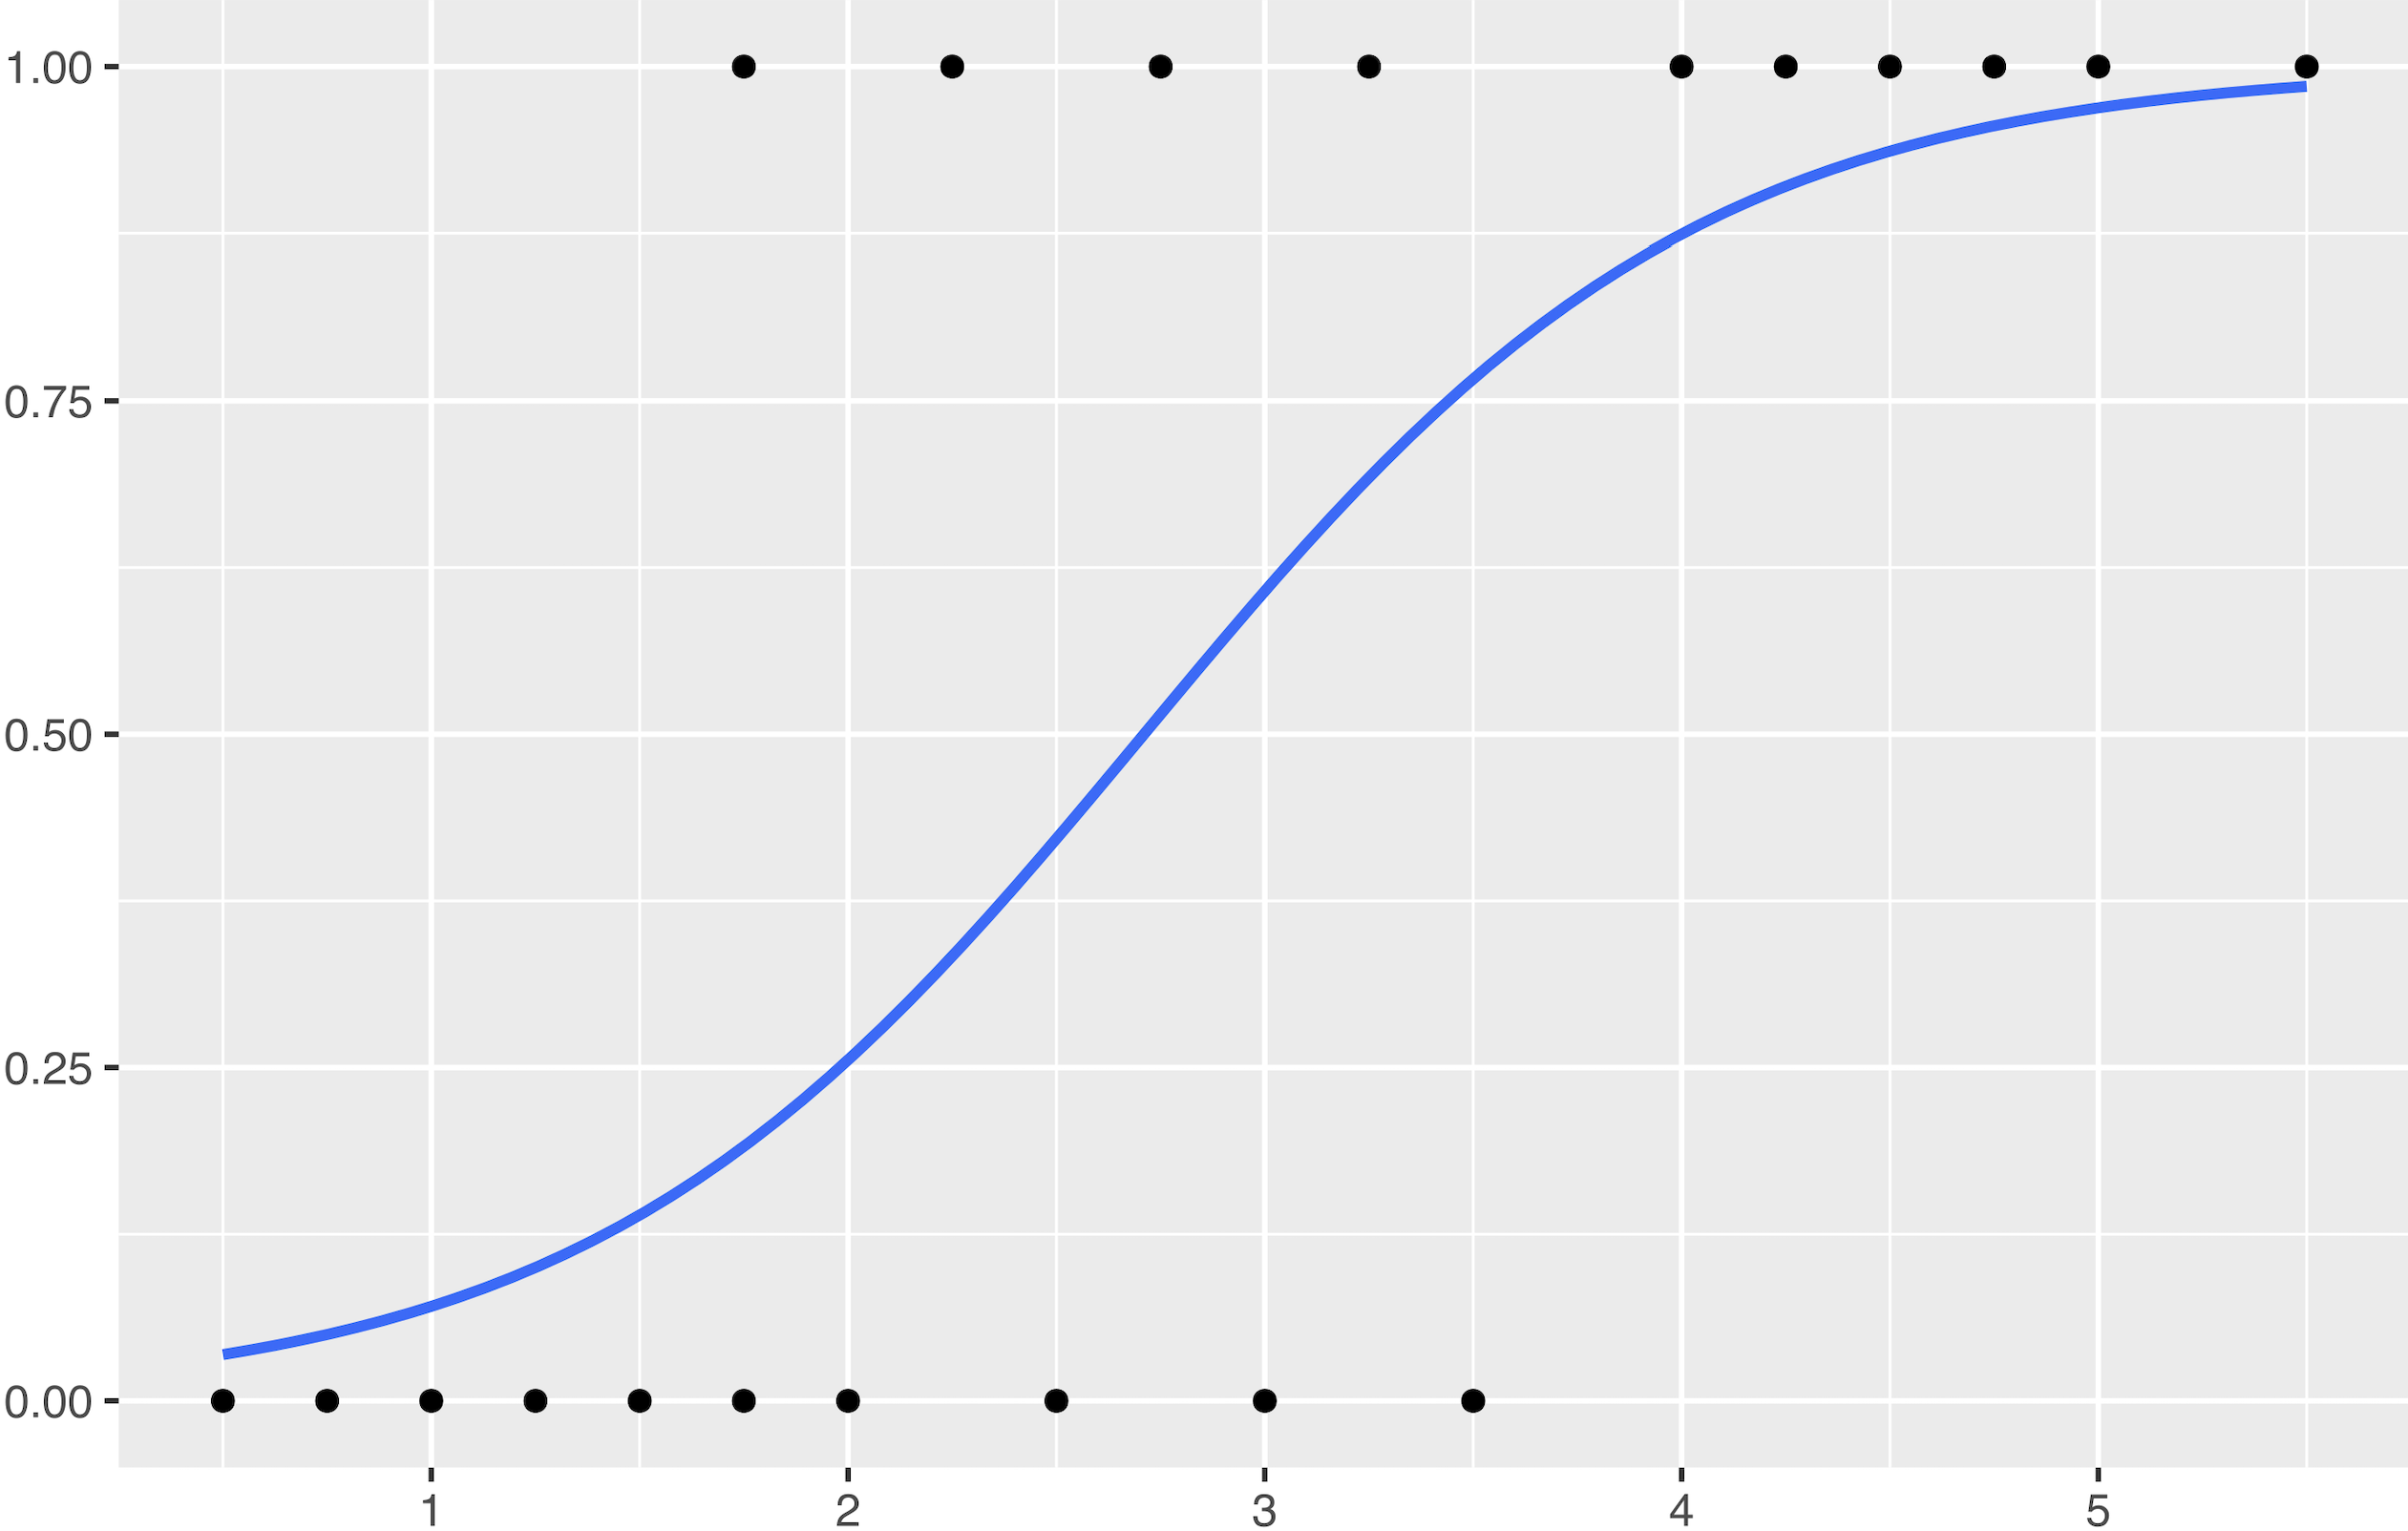
\includegraphics[width=0.6\linewidth]{Logistic Regression.png}
    \caption{Logistic Regression}
    \label{fig:logistic_regression}
\end{figure}

\vspace{1.5cm}

L'altro modello statistico utilizzato \`e stato la \textbf{Linear Discriminant Analysis (LDA)}. Questo modello, cerca di trovare una combinazione lineare di features che separino al meglio le classi nel dataset. La LDA funziona proiettando i dati su uno spazio a minore  dimensionalit\`a che massimizza la separazione tra le classi. Ci\`o avviene trovando un insieme di discriminanti lineari che massimizzano il rapporto tra la varianza inter-classe e la varianza intra-classe \cite{lda}. In altre parole, trova le direzioni nello spazio delle features che meglio separano le diverse classi di dati, nel nostro caso anomalia rilveata o non rilevata.

\begin{figure}[H]
    \centering
    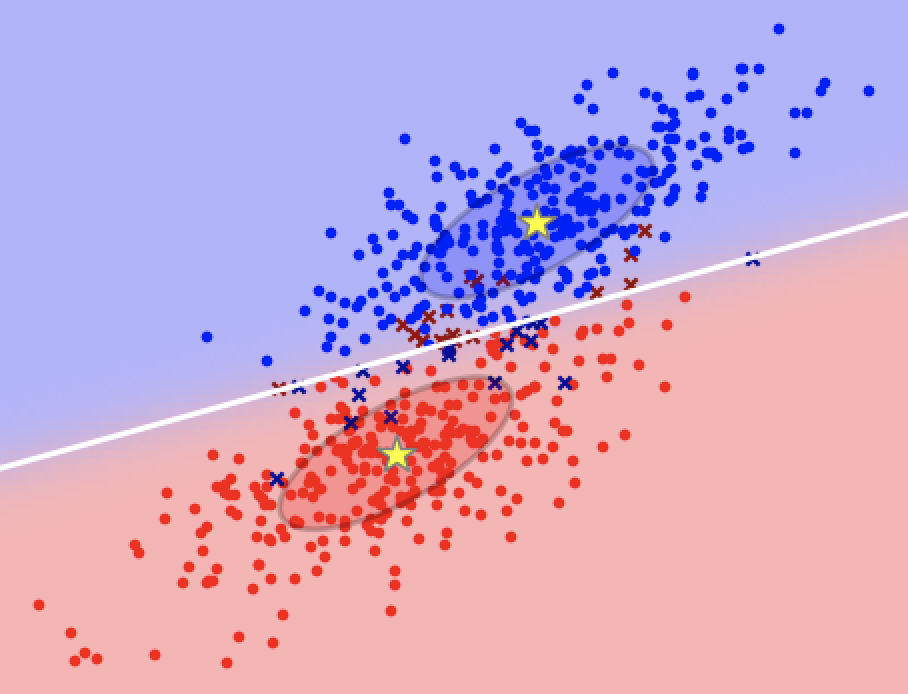
\includegraphics[width=0.5\linewidth]{LDA2.png}
    \caption{Linear Discriminant Analysis}
    \label{fig:lda}
\end{figure}

\subsubsection{{Modelli basati su Alberi Decisionali}}
I modelli non statistici utilizzati sono entrambi basati sugli alberi decisionali, quindi prima di definire i singoli modelli, procederemo con un'introduzione su cosa sono gli alberi decisionali. Un \textbf{Albero Decisionale (DT)} \`e un algoritmo ampiamente utilizzato nell'apprendimento supervisionato, adatto sia per attivit\`a di classificazione che per problemi di regressione. Questo modello adotta una struttura ad albero gerarchica, caratterizzata da un nodo radice, rami, nodi interni e nodi foglia\cite{dt}.
\begin{figure}[H]
    \centering
    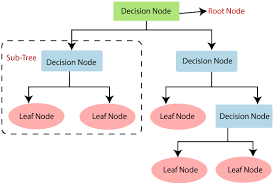
\includegraphics[width=0.6\linewidth]{DT.png}
    \caption{Schema Albero Decisionale}
    \label{fig:enter-label}
\end{figure}

\vspace{1cm}

Come rappresentato nel diagramma soprastante, un Albero Decisionale inizia con un nodo radice, che \`e contraddistinto dalla mancanza di rami in ingresso. I rami che si dipartono dal nodo radice alimentano i nodi interni, noti anche come nodi decisionali.  Sia il nodo radice che i nodi decisionali contribuiscono nella creazione di sottoinsiemi omogenei all'interno del dataset, in particolare, i nodi foglia rappresentano tutte le possibili previsioni o risultati nel set di dati. 
Il training dell'albero decisionale utilizza una strategia "dividi et impera" per cercare i punti di suddivisione ottimali all'interno di un albero.
Vediamo nella figura sottostante un diagramma, molto semplice e a titolo di esempio, di un albero decisionale per determinare la presenza o meno di un'anomalia all'interno di un calcolatore. 

\begin{figure}[H]
    \centering
    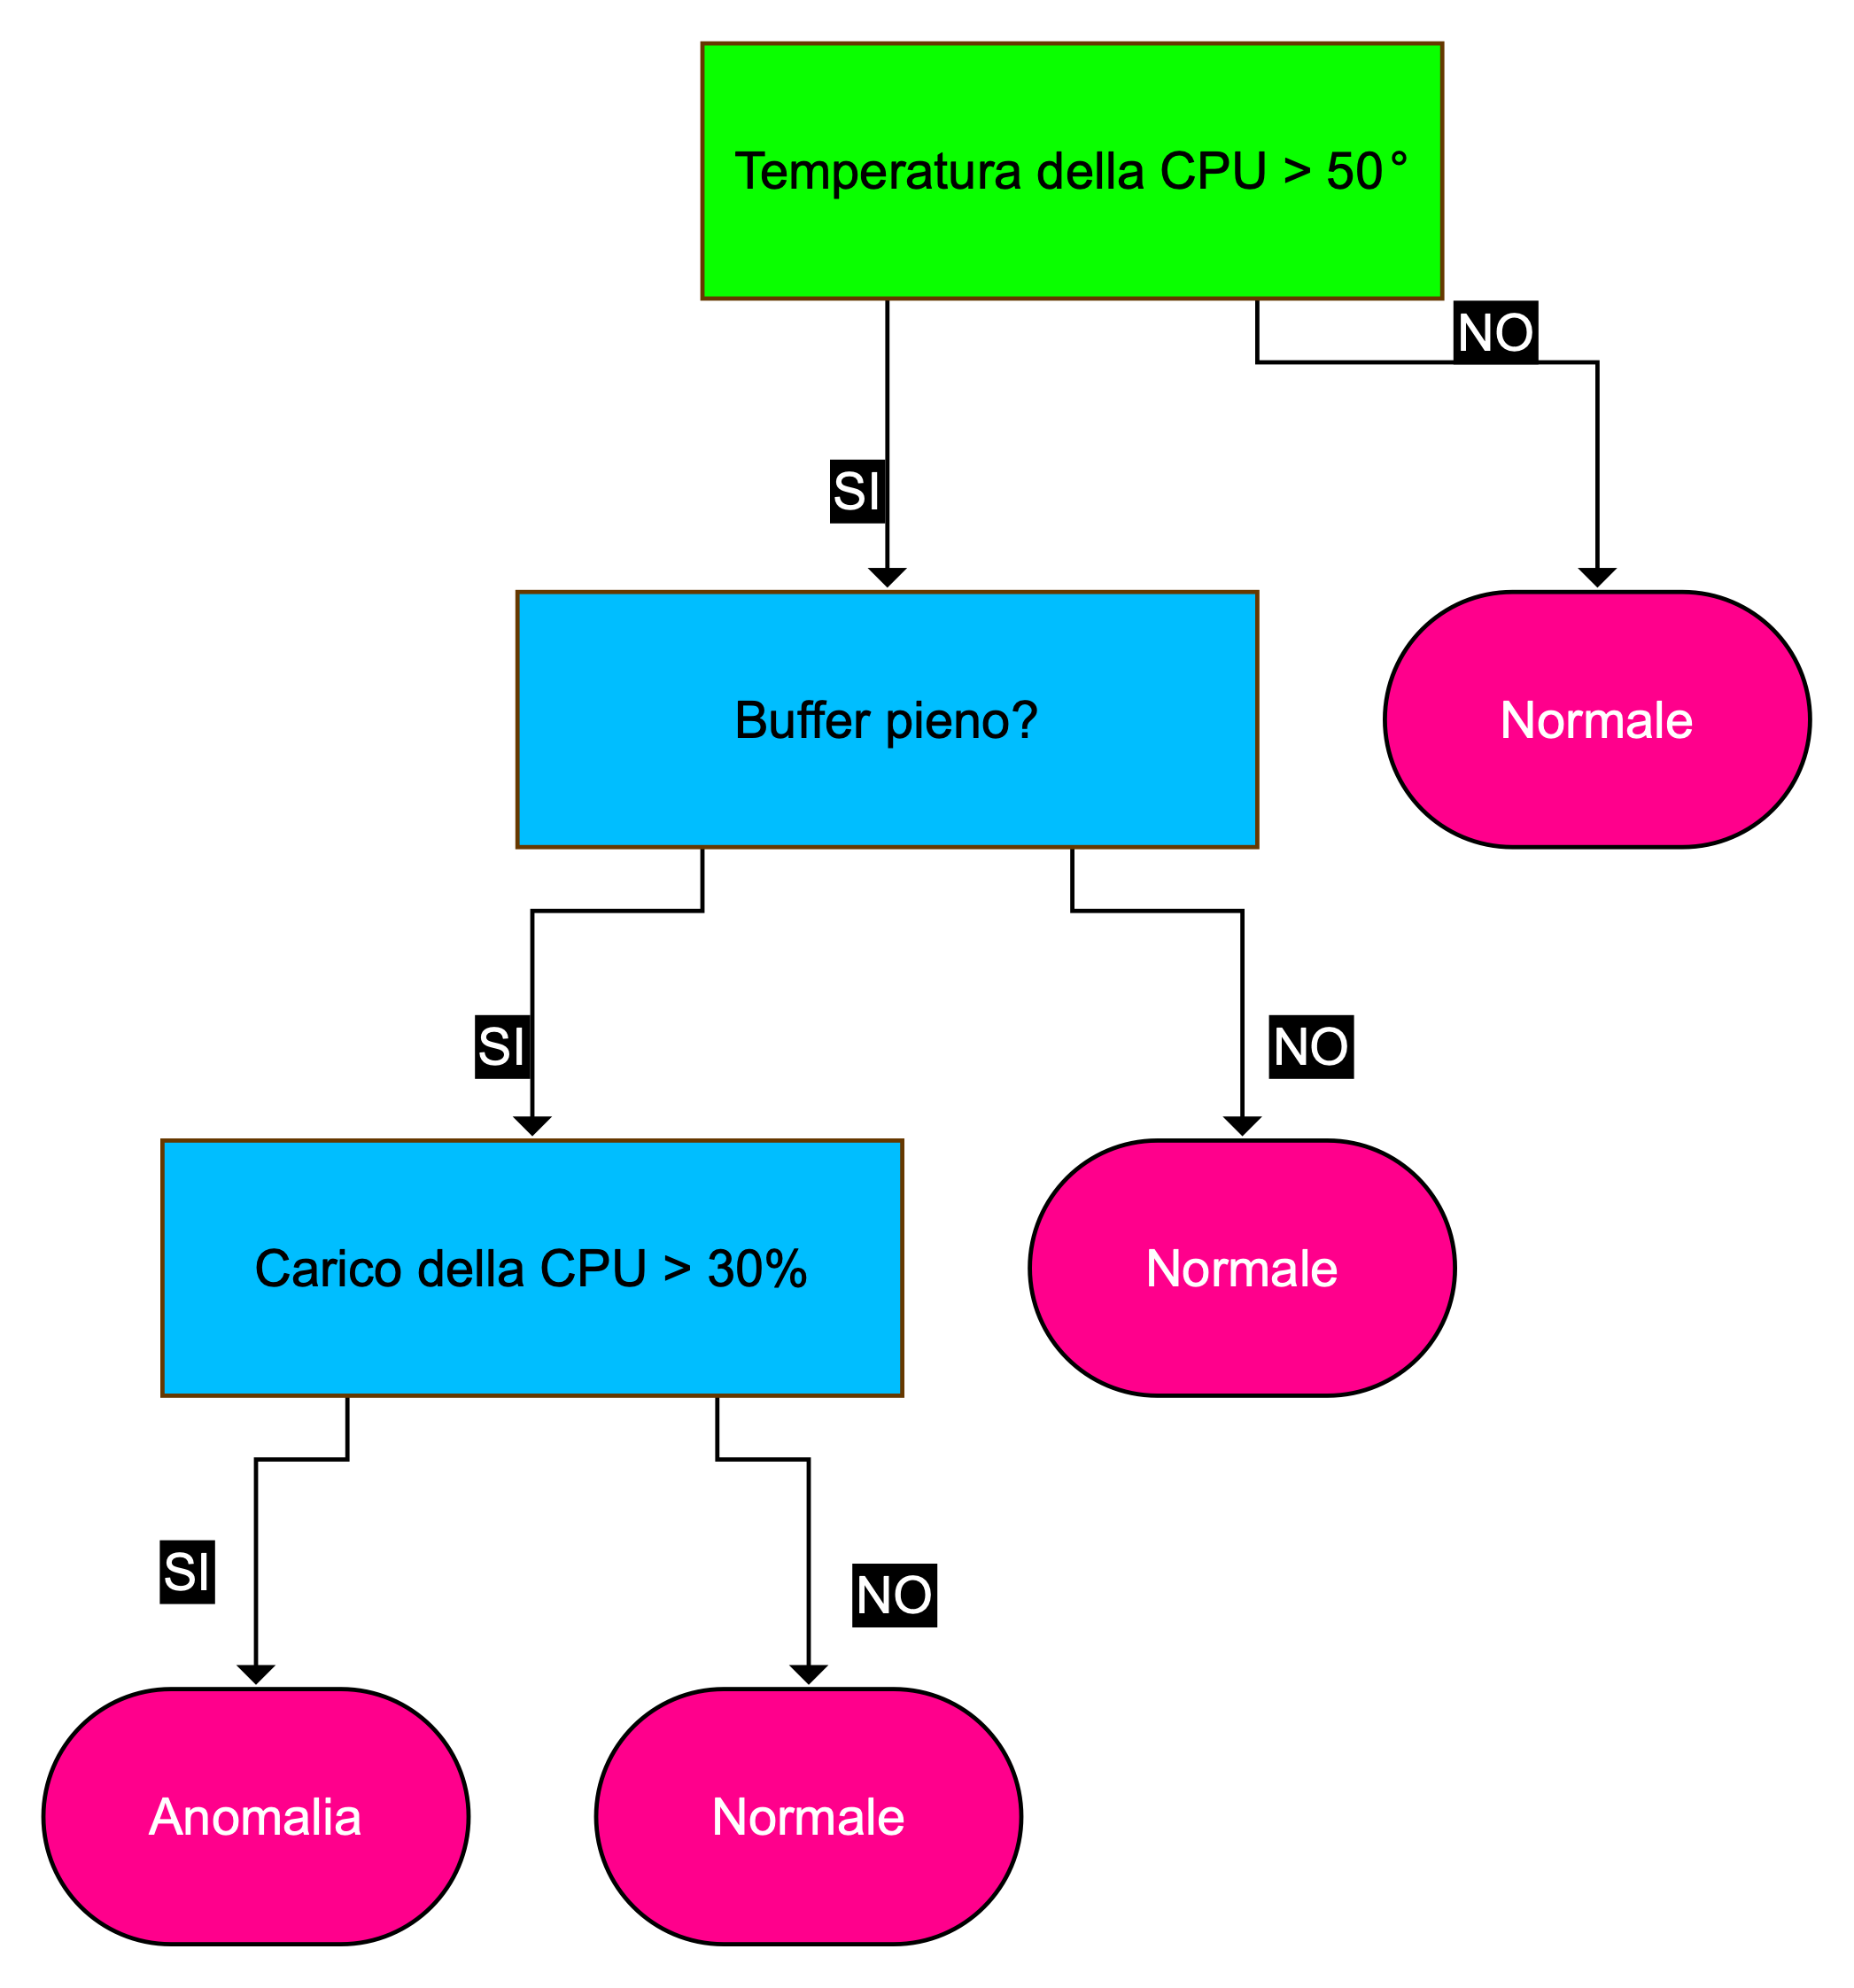
\includegraphics[width=0.6\linewidth]{Esempio DT.png}
    \caption{Esempio Albero Decisionale}
    \label{fig:enter-label}
\end{figure}

\vspace{1cm}

Nel nostro caso non abbiamo usato direttamente degli alberi decisionali, ma dei modelli basati su di essi. L'algoritmo \textbf{Random Forest (RF)} \`e un classificatore d'insieme basato su alberi decisionali, ovvero \`e costituito da un insieme di classificatori, in questo caso DT, e le loro previsioni vengono aggregate per identificare il risultato pi\`u diffuso \cite{rf}.
In particolare, l'algoritmo RF utilizza una tecnica dell'apprendimento d'insieme, chiamata bagging, in cui pi\`u DT vengono addestrati su insiemi di dati diversi, ciascuno ottenuto dal dataset di addestramento iniziale. La casualit\`a delle caratteristiche su cui vengono addestrati i singoli alberi della foresta garantisce una bassa correlazione tra le singole strutture ad albero, riducendo cos\`i uno dei maggiori problemi degli alberi decisionali, l'overfitting. 
L'overfitting \`e un problema che si verifica quando un modello si adatta esattamente ai suoi dati di addestramento. Quando questo accade, l'algoritmo non funziona correttamente in presenza di dati non osservati in precedenza e non \`e quindi in grado di generalizzare, risultando inutile.
Possiamo schematizzare il comportamento dell'algoritmo Random Forest nella figura seguente.

\begin{figure}[H]
    \centering
    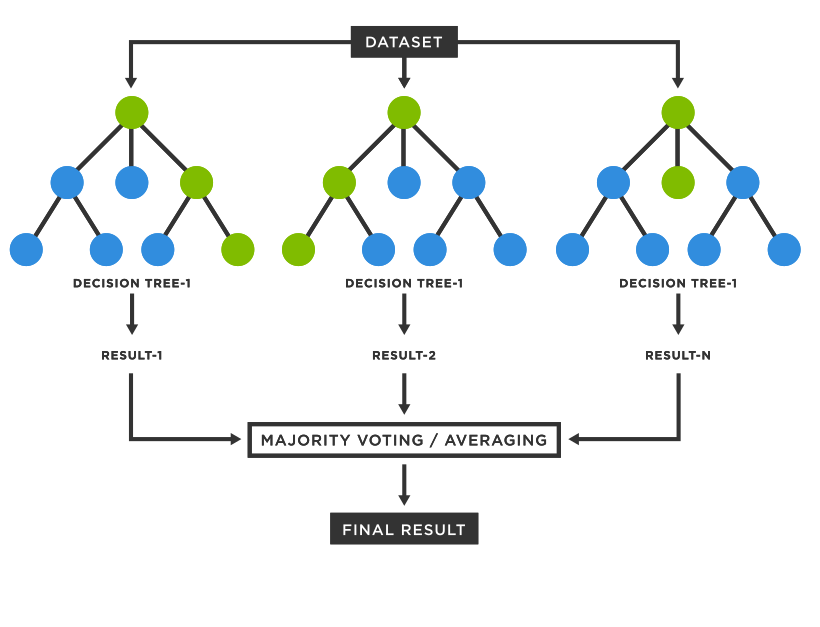
\includegraphics[width=0.6\linewidth]{RF Diagramma.png}
    \caption{Schema Random Forest}
    \label{fig:enter-label}
\end{figure}

Nel nostro caso, ovvero nel caso della classificazione, il risultato del modello corrisponder\`a al voto di maggioranza dei singoli alberi sulla classe prevista.

\vspace{1.7cm}

L'altro algoritmo basato su alberi decisionali utlizzato nel presente lavoro di Tesi \`e \textbf{XGBoost}, il cui nome completo \`e Extreme Gradient Boosting. Solitamente l'approccio pi\`u frequente quando si costruiscono dei modelli predittivi \`e addestrare un singolo modello forte. Un approccio differente potrebbe essere quello di costruire un insieme di modelli deboli che combinati costruiscano una previsione d'insieme forte. Quest'ultima idea \`e alla base di tutti gli algoritmi di ensemble learning, quindi anche di XGBoost e Random Forest \cite{gradient_boost}.
Come si deduce dal nome dell'algoritmo, XGBoost \`e basato sul boosting, ovvero un metodo di apprendimento d'insieme, proprio come lo \`e il bagging per Random Forest. Il boosting combina una serie di modelli deboli che vanno a formare un modello forte per ridurre al minimo gli errori di addestramento \cite{xgb}. Nel boosting, viene effettuata una selezione casuale dal set di dati e il modello viene addestrato in modo sequenziale, ovvero ogni modello successivo nella sequenza cerca di migliorare rispetto al precedente. I modelli deboli, che non sono nient'altro che alberi decisionali, vengono combinati per ottenere una previsione d'insieme forte. La differenza principale con la tecnica di bagging utilizzata da Random Forest \`e che nel bagging i modelli deboli sono addestrati in parallelo, mentre nel boosting apprendono in sequenza. Il miglioramento dei modelli durante l'apprendimento sequenziale avviene grazie all'algoritmo di discesa del gradiente (notare il termine \textit{Gradient} in  \textit{Extreme Gradient Boosting}), ovvero un algoritmo di ottimizzazione molto utilizzato nel ML.
XGBoost (Extreme Gradient Boosting) \`e un'implementazione di Gradient Boosting, nome utilizzato poich\'e combina l'algoritmo di discesa del gradiente e il metodo di boosting, progettata per velocit\`a e scalabilit\`a.


\subsection{Metriche di valutazione}
In questa sezione illustriamo le metriche di valutazione utilizzate per valutare le performance dei modelli. Prima di menzionare le singole metriche, \`e necessario introdurre il concetto di \textit{confusion matrix (matrice di confusione)}. La matrice di confusione \`e una matrice utilizzata per valutare le prestazioni di un algoritmo di ML, che pu\`o essere cos\`i schematizzata \cite{mcc}:

\begin{figure}[H]
    \centering
    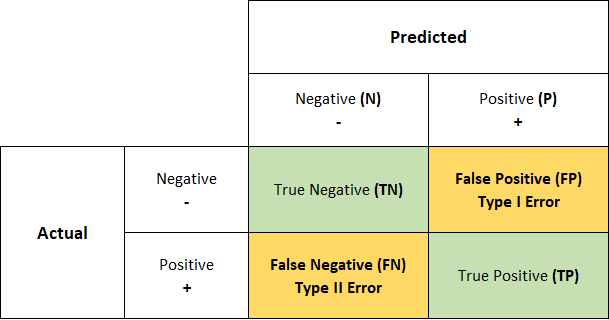
\includegraphics[width=0.5\linewidth]{confusion_matrix.png}
    \caption{Confusion Matrix}
    \label{fig:enter-label}
\end{figure}

Ora che abbiamo introdotto la confusion matrix possiamo meglio definire le metriche di valutazione. In totale sono state utilizzate 4 metriche di valutazione:

\begin{itemize}

  \item \textbf{Accuracy (ACC)}: il valore \`e dato dal numero delle classificazioni corrette diviso il numero totale di classificazioni. Formalmente, guardando alla confusion matrix, il valore \`e dato da:

  \begin{equation}
    ACC = \frac{TP + TN}{P + N}
  \end{equation}
  
  \item \textbf{Error Rate (1-ACC)}: il valore \`e dato dalla differenza tra 1 e l'Accuracy, ovvero $1-ACC$
  
  \item \textbf{Matthews correlation coefficient (MCC)}: questa metrica di valutazione, rispetto alle precedenti, \`e sicuramente la pi\`u robusta per valutare le performance dei modelli. Questo perch\'e, a differenza dell'accuracy, questa metrica non \`e affetta dal problema degli \textit{unbalanced datasets (set di dati sbilanciati)}, ma torneremo su questo problema tra poco. Guardando alla matrice di confusione il valore dell'MCC \`e dato da:
  
  \begin{equation}
      MCC = \frac{TP \cdot TN - FP \cdot FN}{\sqrt{(TP + FP)(TP + FN)(TN + FP)(TN + FN)}}
  \end{equation}

  
  \item \textbf{Speed Score (SS)}: questa metrica \`e stata creata ed utilizzata appositamente per analizzare le performance dei nostri modelli sui dataset usati nel lavoro di Tesi. Lo scopo di questa metrica \`e quello di misurare la velocit\`a con cui il modello rileva l'anomalia. Ovviamente nell'Anomaly Detection \`e molto importante che le anomalie vengano rilevate nel minor tempo possibile. Per comprendere la formula del SS basta sapere che le anomalie sono sempre presenti per 5 istanti di tempo (5 secondi), ovvero 5 righe del dataset (la descrizione del dataset nel dettaglio \`e presente nel Capitolo 3). La formula per lo speed score \`e una somma pesata delle frequenze di rilevamento con decrescita quadratica e non lineare, per dare maggiore importanza alle rilevazioni nei primi istanti di tempo, diviso il totale delle anomalie rilevate.
  
    \begin{equation}
      SS = \frac{x_0 \cdot 1 + x_1 \cdot 0.8^2 + x_2 \cdot 0.6^2 + x_3 \cdot 0.4^2 + x_4 \cdot 0.2^2}{TotaleAnomalie}
    \end{equation}

    Con $x_0, x_1, x_2, x_3, x_4$ che indicano rispettivamente il numero di anomalie rilevata al primo, secondo, terzo, quarto e quinto istante di tempo.
\end{itemize}

\vspace{1.5cm}

Riprendiamo per un momento il problema degli unbalanced datasets. Questo problema avviene quando, in una classificazione binaria ad esempio,la frequenza di una delle due etichette risulta sbilanciata rispetto all'altra, ovvero una delle due etichette risulta molto pi\`u frequente nel dataset rispetto all'altra. Per comprendere al meglio il problema facciamo un esempio che risalti gli aspetti critici degli unbalanced datasets. Supponiamo di avere un dataset dove il 95\% dei dati \`e etichettato come 'normale', mentre il restante 5\% \`e etichettato come 'anomalia'. Se avessimo un modello chiamato \textit{dumb model} che classifica come 'normale' tutti i dati in input, avrebbe un'ACC del 95\% sul nostro dataset. Se prendessimo l'ACC come metrica di riferimento, il nostro dumb model sembrerebbe un ottimo classificatore di anomalie, quando a stento potremmo definirlo classificatore. Abbiamo preso quindi l'MCC come metrica di riferimento perch\'e molto pi\`u robusta, non risentendo degli effetti dei set di dati sbilanciati.
    
\begin{figure}[H]
    \centering
    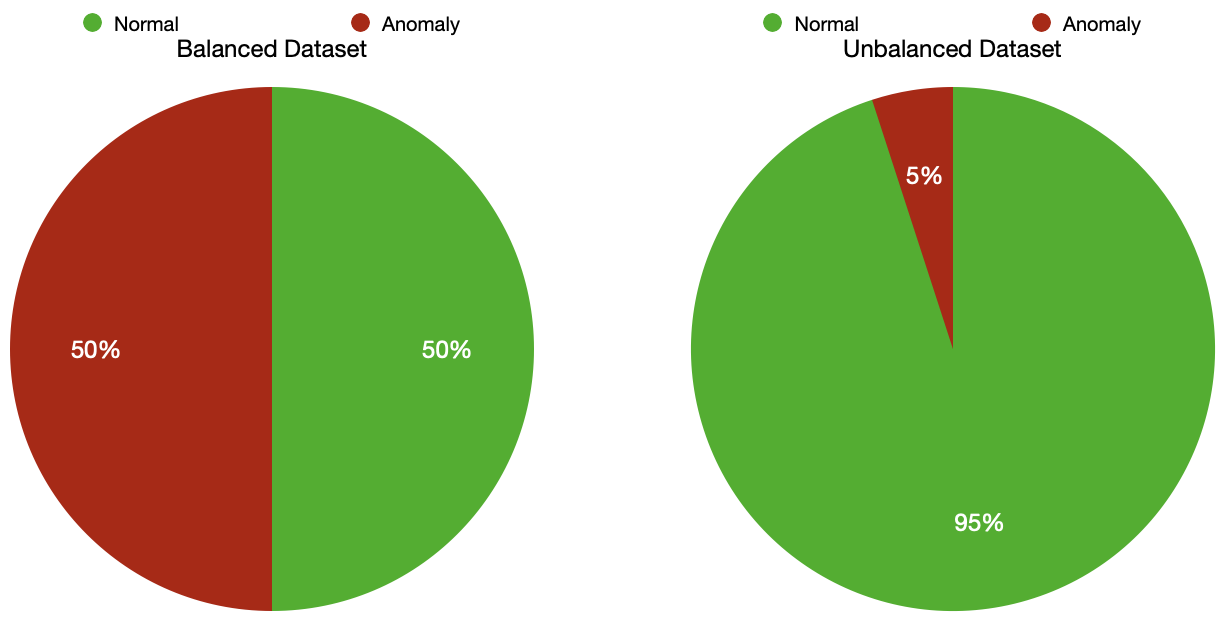
\includegraphics[width=0.7\linewidth]{Balanced_Unbalanced_Dataset.png}
    \caption{Balanced e Unbalanced Datasets}
    \label{fig:enter-label}
\end{figure}

\vspace{1cm}

\section{Anomaly Detection}
L'\textit{Anomaly Detection} (o \textit{rilevamento di anomalie} in italiano) consiste nella rilevazione di eventi rari che non rientrano nella definizione di comportamento normale dei dati. Il rilevamento di anomalie \`e particolarmente importante nel settore della sicurezza informatica, ma anche nei settori quali finanza, medicina e molti altri ancora. 


\begin{figure}[H]
    \centering
    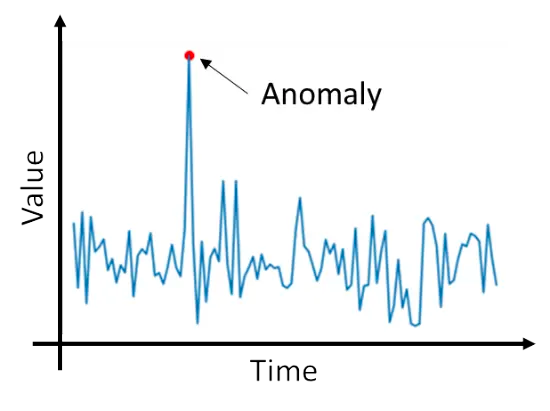
\includegraphics[width=0.6\linewidth]{anomalie.png}
    \caption{Esempio Anomalia}
    \label{fig:enter-label}
\end{figure}


Un tempo chi si occupava di anomaly detection era solito eseaminare manualmente i dati, alla ricerca di comportamenti fuori dal normale, spesso non trovando le cause principali delle anomalie. Ad oggi il rilevamento di anomalie si basa quasi totalmente sul machine learning. Per definizione le anomalie sono eventi rari e quindi avremo a che fare spesso con dataset sbilanciati, con maggior presenza di dati etichettati come 'normali' rispetto a quelli etichettati come 'anomalie'.
Le 3 categorie principali di tecniche di anomaly detection sono \cite{anomaly} :

\begin{itemize}

  \item \textbf{Anomaly Detection Supervisionata}: richiedono un set di dati etichettato in due classi, 'normale' e 'anomalia', e implicano l'addestramento di un classificatore. \`E il caso preso in analisi nel presente lavoro di Tesi.
  
  \item \textbf{Anomaly Detection Semi-Supervisionata}: richiedono che una porzione dei dati sia etichettata.

  \item \textbf{Anomaly Detection Non Supervisionata}: i dati non sono etichettati e sono sicuramente le tecniche pi\`u diffuse oggigiorno.

  
    
\end{itemize}

\section{Time Series}
Il tempo \`e una variabile fondamentale per fare delle previsioni sul futuro. Per introdurre questo fattore nei nostri modelli ricorriamo alle \textit{Time Series}(o \textit{serie storiche} in italiano), che definiamo come un insieme di osservazioni ordinate rispetto al tempo \cite{time_series}. L'analisi delle serie storiche non coincide meramente con l'atto di raccogliere e analizzare dati nel tempo. Ci\`o che contraddistingue una serie strorica da altri tipi di dati \`e che in una serie storica \`e possibile vedere come le variabili o features cambino nel tempo. Il tempo \`e una variabile cruciale e fornisce delle informazioni aggiuntive per i modelli.
Le serie storiche vengono solitamente analizzate con modelli specifici per \textit{time series forecasting}, che consiste nell'utilizzare un modello per predire valori futuri basandosi sui valori precedentemente osservati , come ad esempio il modello ARIMA. In letteratura, difficilmente vengono utilizzati algoritmi di ML come Random Forest o XGBoost per l'analisi di serie storiche \cite{time_series_link}. Quello che ci siamo proposti in questo lavoro di Tesi \`e stato unire un problema di classificazione binaria (Anomaly Detection Supervisionata) con un approccio time series per dare maggiori informazioni ai modelli in fase di training, aspettandoci un miglioramento nelle performance dei modelli stessi.

 \vspace{-0.5cm}
 \vspace{-0.3cm}

\chapter{Metodologie}

\medskip

\section{Descrizione Dataset}
I dataset utilizzati nel presente lavoro di Tesi sono il risultato della ricerca dell'articolo (*commento per il Professore: non credo che il paper sia gi\`a stato pubblicato, posso citarlo?*) qui citato \cite{zoppi}. Le features contenute nel dataset sono state ottenute monitorando degli indicatori di performance di un dispositivo chiamato ARANCINO \cite{arancino}, che \`e il nome commerciale per una famiglia di schede IoT e embedded che risiedono sull'omonima architettura. In istanti di tempo casuali, il dispositivo \`e stato sottoposto a delle \textit{error injections} della durata costante di 5 secondi. Gli errori con cui \`e stato attaccato il dispositivo sono di 8 tipi:

\begin{itemize}
    \item CPU usage
    \item RAM usage
    \item Deadlock
    \item Redis read
    \item Redis write
    \item Stuck arancino
    \item Stuck node-red
\end{itemize}


Gli indicatori di performance monitorati sono stati presi a livello hardware, a livello di sistema, dai sensori, dall'ambiente e a livello di applicazione. In particolare le feature presenti nel dataset possono essere suddivise nelle seguenti 7 categorie:

\begin{itemize}
    \item Network: 32 features
    \item Chip Temperature: 1 feature
    \item Virtual Memory: 116 features
    \item Memory Info: 38 features
    \item IO Stats: 6 features
    \item Python Indicators: 55 features
    \item Redis DB: 25 features
\end{itemize}

Ogni osservazione \`e dotata di un'etichetta che fornisce l'informazione sullo stato del dispositivo: normale o anomalo (durante le \textit{error injections}). Se lo stato \`e normale l'etichetta corrisponder\`a a 'normal' altrimenti sar\`a una stringa che descrive l'\textit{error injection} perpetrata in quel momento nel sistema.
I dataset a disposizione sono stati:
\begin{itemize}
    \item \textit{unifi-filtered}: 69000 osservazioni. Il dispositivo \`e connesso al WiFi dell'Universit\`a degli Studi di Firenze.
    \item \textit{homenet-filtered}: 72000 osservazioni. Il dispositivo \`e connesso al WiFi di un appartamento residenziale.
    \item \textit{mobile-filtered}: 13000 osservazioni. Il dispositivo \`e connesso a una WiFi privata (ad esempio usando il tethering da una connessione mobile).
    \item \textit{all3}: 154000 osservazioni, \`e l'unione dei primi 3 dataset
\end{itemize}


\subsection{Dataset unifi-filtered}
Il dataset su cui sono stati addestrati i modelli \`e \textit{unifi-filtered}. Sono presenti 69000 osservazioni totali, di cui 11989 osservazioni etichettate come anomalie.

\begin{figure}[H]
    \centering
    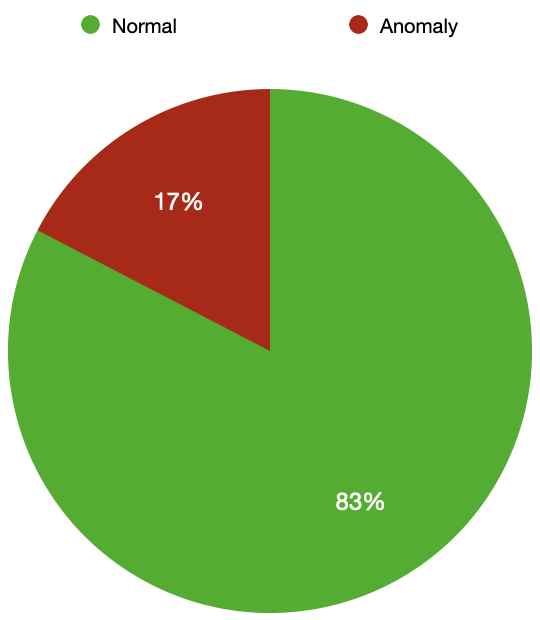
\includegraphics[width=0.5\linewidth]{balance_unifi.png}
    \caption{Composizione Dataset unifi-filtered}
    \label{fig:enter-label}
\end{figure}



\subsection{Dataset all3}
Il dataset \textit{all3} \`e stato utilizzato come test set per valutare le performance dei modelli su istanze diverse del problema. In realtà, non \`e stato utilizzato il dataset \textit{all3}, ma una sua versione modificata. Avendo \textit{all3} tutte le osservazioni al suo interno, comprese quelle su cui sono stati addestrati i modelli, se fosse stato utilizzato come test set avremmo testato i modelli anche su input su cui erano gi\`a stati addestrati, ottenendo come risultato delle metriche inaccurate. Per risolvere questo problema abbiamo creato una versione custom di \textit{all3} chiamata \textit{my-all3}, unendo il dataset \textit{homenet-filtered} e \textit{mobile-filtered} con solo il set di dati di test di \textit{unifi-filtered}, senza i dati di addestramento.
In \textit{my-all3} sono presenti 105700 osservazioni totali, di cui 18245 etichettate come anomalie.

\begin{figure}[H]
    \centering
    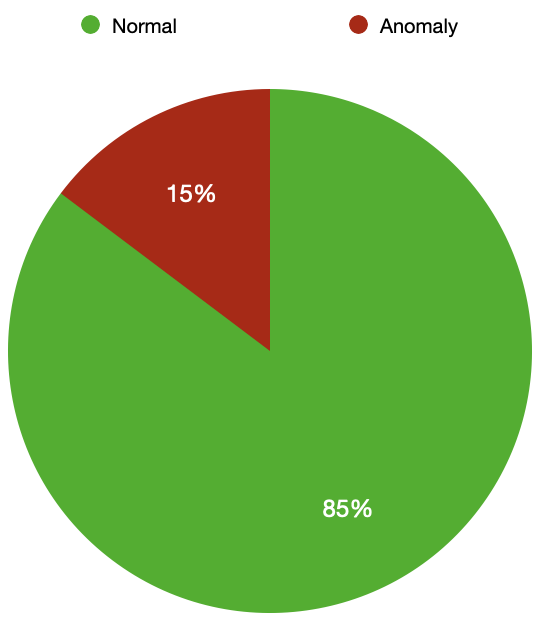
\includegraphics[width=0.5\linewidth]{balance_myall3.png}
    \caption{Composizione Dataset my-all3}
    \label{fig:enter-label}
\end{figure}



\section{Preprocessing}
I dataset utilizzati erano gi\`a stati in parte preprocessati, ad esempio non erano presenti righe con valori NaN e i dati categorici erano gi\`a stati convertiti in dati numerici.
Le operazioni di preprocessing aggiuntive sono state:

\begin{itemize}
    \item Eliminazione delle feature con valori costanti. Ad esempio erano presenti features in cui il valore non variava mai e rimaneva sempre uguale a 1, quindi non fornivano nessuna informazione utile ai modelli.
    \item Trasformazione delle etichette con la descrizione delle diverse anomalie in \textit{'anomaly'}. In questo modo \`e stato trasformato un problema di classificazione multiclasse in un problema di classificazione binaria.
    \item Mapping delle etichette da \textit{'normal'} e \textit{'anomaly'} a 0 e 1, rispettivamente. In questo modo anche l'etichetta \`e diventata un valore numerico e abbiamo soltanto dati numerici nel dataset.
\end{itemize}

\begin{figure}[H]
    \centering
    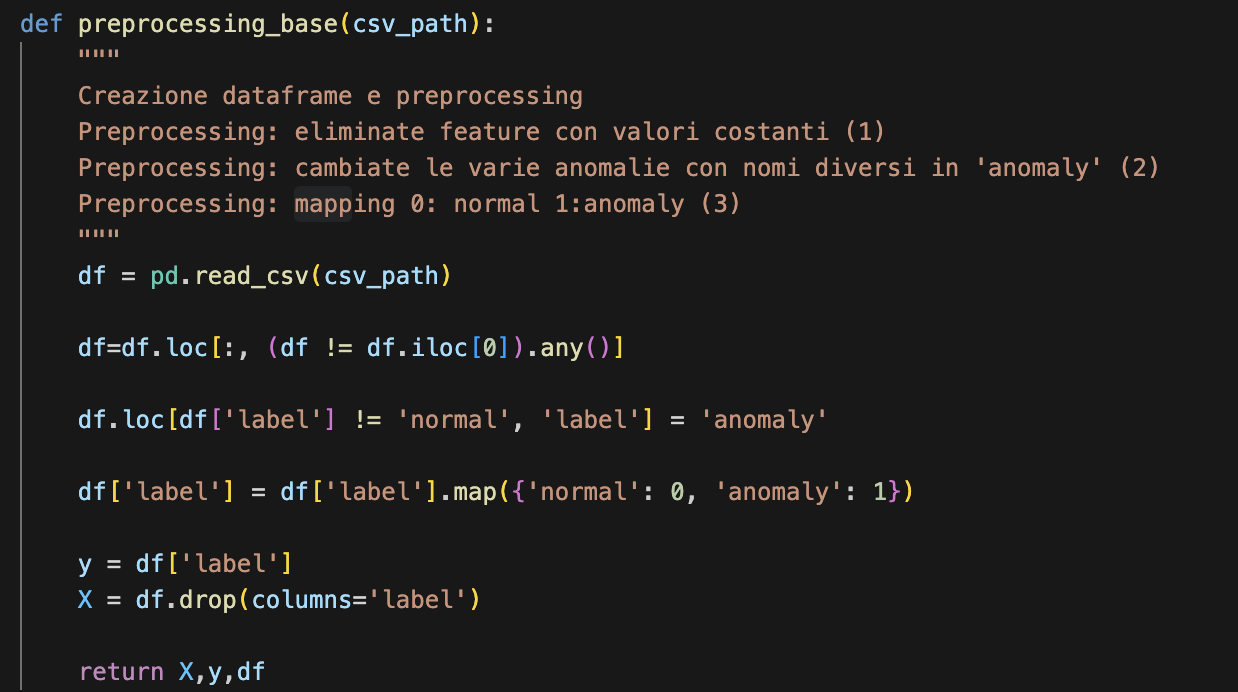
\includegraphics[width=0.9\linewidth]{preprocessing.png}
    \caption{Funzione per preprocessing datasets}
    \label{fig:enter-label}
\end{figure}

L'ultima operazione di preprocessing \`e stata standardizzare i dataset attraverso l'utilizzo della classe \textit{StandardScaler()} presente nel modulo \textit{scikit-learn}. Questa operazione di preprocessing permette di elaborare la riduzione in scala dei dati, trasformando le serie di valori in una distribuzione normale standard con media uguale a 0 e deviazione standard uguale a 1 \cite{stdscaler}. Standardizzare i dati \`e un'operazione di preprocessing con la quale solitamente si ottengono delle performance migliori nel processo di apprendimento.

\section{Strategie}
Le strategie adottate per l'addestramento dei modelli sono state 3 in totale. Un approccio classico, senza alcuna modifica al dataset \textit{unifi-filtered}, e 2 approcci time series, intervenendo sulla struttura del dataset. In generale per ogni modello \`e stato calcolato l'MCC, lo speed score e infine l'accuracy tramite cross-validation. Inoltre \`e stata graficata per tutti i modelli la progressione delle metriche appena menzionate rispetto agli approcci utilizzati. \`E stato graficato anche un confronto tra la progressione dei valori di MCC calcolati sul test set di \textit{unifi-filtered} e quella su \textit{my-all3}.

\subsection{Approccio Classico}
Nell'approccio classico \`e stato effettuato il training dei 4 modelli, che ricordiamo essere Logistic Regression, Linear Discriminant Analysis, Random Forest e XGBoost, sul dataset \textit{unifi-filtered} senza alcuna modifica, a parte le operazioni di preprocessing.

\subsection{Approccio Time Series con Media Mobile}
La media mobile semplice (SMA, \textit{simple moving average}) \`e un indicatore molto utilizzato nell'analisi di serie storiche, questo perch\'e ogni punto della media mobile porta con s\'e l'informazione di $n$ istanti di tempo precedenti. Diamo la definizione di media mobile semplice: data una serie storica $y_t$ con $t=1,2,...T$ contenente i valori osservati di una variabile $Y$ dal tempo 1 al tempo $T$ si definisce media mobile al tempo $t$ il valore \cite{sma}:

  \begin{equation}
      SMA=\frac{1}{k} \sum_{i=-m_1}^{m_2} y_{i+1}
  \end{equation}
dove $k=m_1+m_2+1$ \`e il periodo della media mobile, ed equivale al numero degli addendi.

Entrambi gli approcci time series, sia con media mobile che con differenze, sono stati ottenuti andando a modificare i dataset, aggiungendo delle nuove features che portassero dell'informazione time series con loro.
Il primo approccio sperimentato \`e stato quello di creare per ogni feature presente nel dataset una feature aggiuntiva che contenesse il valore della media mobile semplice (SMA) di $n$ istanti precedenti. In questo modo i modelli sono stati addestrati sul doppio delle feature, dato che per ogni \textit{feature} \`e stata creata la corrispondente feature \textit{feature-media-mobile}, con a disposizione le importanti informazioni su come i valori delle feature siano evoluti nel tempo. 

\begin{figure}[H]
    \centering
    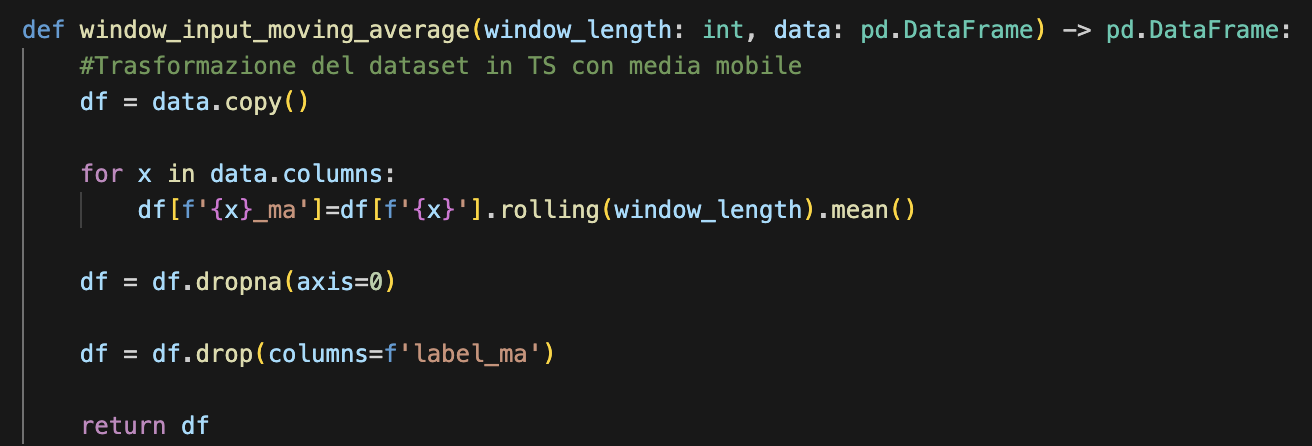
\includegraphics[width=0.9\linewidth]{def_ts_ma.png}
    \caption{Funzione per trasformazione dataset con features media mobile}
    \label{fig:enter-label}
\end{figure}

 
\subsection{Approccio Time Series con Differenze}
Un altro modo di portare informazioni time series all'interno del dataset \`e quello di aggiungere delle nuove feature che contengano la differenza tra il valore attuale delle feature e il loro valore precedente. Anche in questo caso, come per la media mobile, le differenze sono state calcolate su $n$ istanti di tempo, quindi per ogni feature sono presenti altre $n$ feature che rappresentano la differenza tra il valore attuale all'istante $t$ e i valori all'istante $t-1,t-2,...t-n$.

\begin{figure}[H]
    \centering
    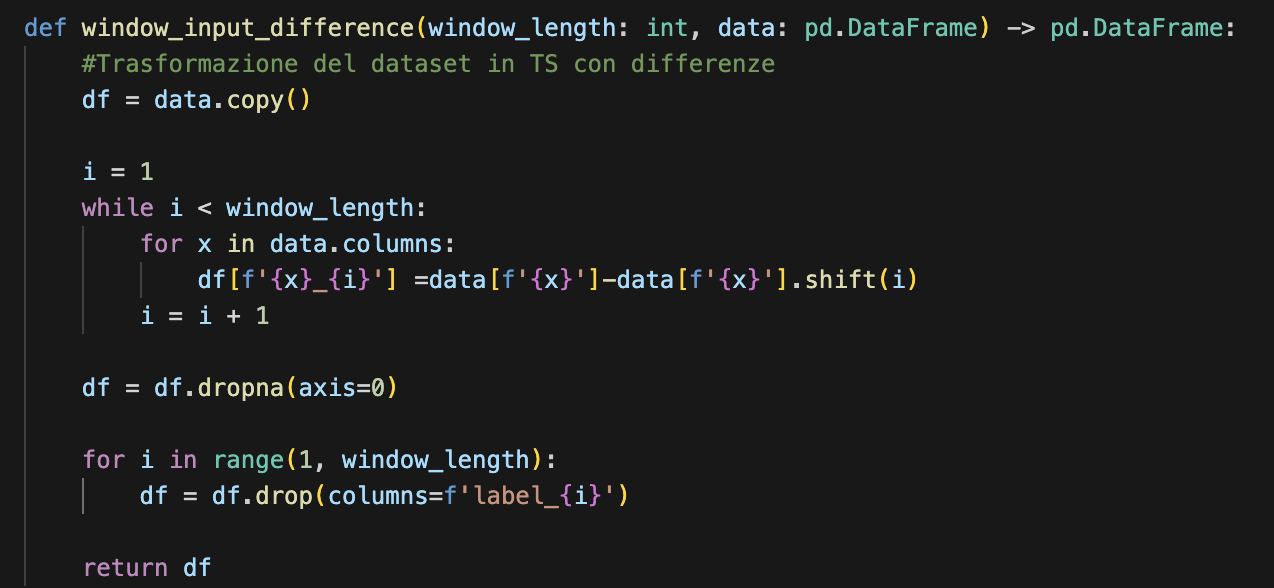
\includegraphics[width=0.9\linewidth]{def_ts_diff.png}
    \caption{Funzione per trasformazione dataset con features differenze}
    \label{fig:enter-label}
\end{figure}

\section{Window e Shuffle}
Gli approcci finora descritti sono stati valutati insieme a due parametri molto importanti: \textit{window} (nel codice \textit{window\_length}) e \textit{shuffle}. \textit{Window} \`e il nome dato al parametro che definisce la finestra temporale, ovvero il numero di istanti di tempo, su cui vengono calcolate la media mobile e le differenze negli approcci time series. La funzione \textit{train\_test\_split} \`e stata utilizzata per dividere il dataset in set di training e set di test e il parametro \textit{shuffle} \`e un parametro booleano che stabilisce se rimescolare o meno i dati prima della suddivisione in train set e test set \cite{train_test_split}.

\subsection{Window}
Negli approcci time series sono stati utilizzati diversi valori per il parametro \textit{window} e quindi per la finestra temporale. Per i valori da assegnare a \textit{window} \`e stato scelto un intervallo $[2,5]$. Per chiarezza, con $window=2$ nel caso delle differenze viene aggiunta al dataset 1 feature per ogni feature presente con la differenza tra il valore all'istante $t$ e il valore all'istante $t-1$, mentre nel caso della media mobile la media sar\`a calcolata tra i valori agli istanti di tempo $t$ e $t-1$. Con $window=5$ nel caso delle differenze verranno aggiunte al dataset 4 feature per ogni feature presente con le differenze tra il valore all'istante $t$ e il valore gli istanti $t-1,t-2,t-3,t-4$, mentre per la media mobile la media sar\`a calcolata tra i valori agli istanti $t,t-1,t-2,t-3,t-4$.
L'intervallo $[2,5]$ \`e stato scelto perch\'e 2 rappresenta la finestra temporale minima e 5 \`e il numero di secondi per cui le anomalie si protraggono all'interno del sistema.
Lo scopo \`e stato quello di verificare come le performance dei modelli andassero a cambiare al variare della finestra temporale.

\subsection{Shuffle}
In generale non \`e appropriato rimescolare i dati quando si tratta di dati time series. Questo perch\'e ci\`o che contraddistingue i dati time series dagli altri tipi di dati \`e che i dati sono raccolti nel tempo e c'\`e correlazione tra osservazioni adiacenti, quindi preservare l'ordine dei dati \`e importante. Per questo di default durante i vari training dei modelli il parametro \textit{shuffle} \`e sempre stato impostato a \textit{False}. Abbiamo comunque voluto verificare quali fossero le differenze di performance dei modelli con il parametro $shuffle=True$. Da notare che con un valore diverso di \textit{shuffle} cambiano i dati nel set di training del modello e quindi si hanno performance e feature importance diverse.

 \vspace{-0.5cm}
 \vspace{-0.3cm}

\chapter{Analisi Risultati}

\medskip

\section{Progressione MCC, Error Rate e Speed Score}

\section{MCC dataset All3}

\section{Progressione MCC al variare della finestra temporale}

\section{Confronto shuffle True/False}

 \vspace{-0.5cm}
 \vspace{-0.3cm}

\chapter{Conclusioni}

\medskip

NULL

 \vspace{-0.5cm}
 \vspace{-0.3cm}
\begin{appendices}
\chapter{Codice Sviluppato}
Il codice sviluppato per il lavoro di Tesi \`e presente al seguente link: \url{https://github.com/xaldvp/Tesi_Triennale}, inoltre sono disponibili tutte le risorse prodotte dal codice, come grafici e file csv. Di seguito viene riportato il codice sviluppato.

\begin{figure}[H]
    \centering
    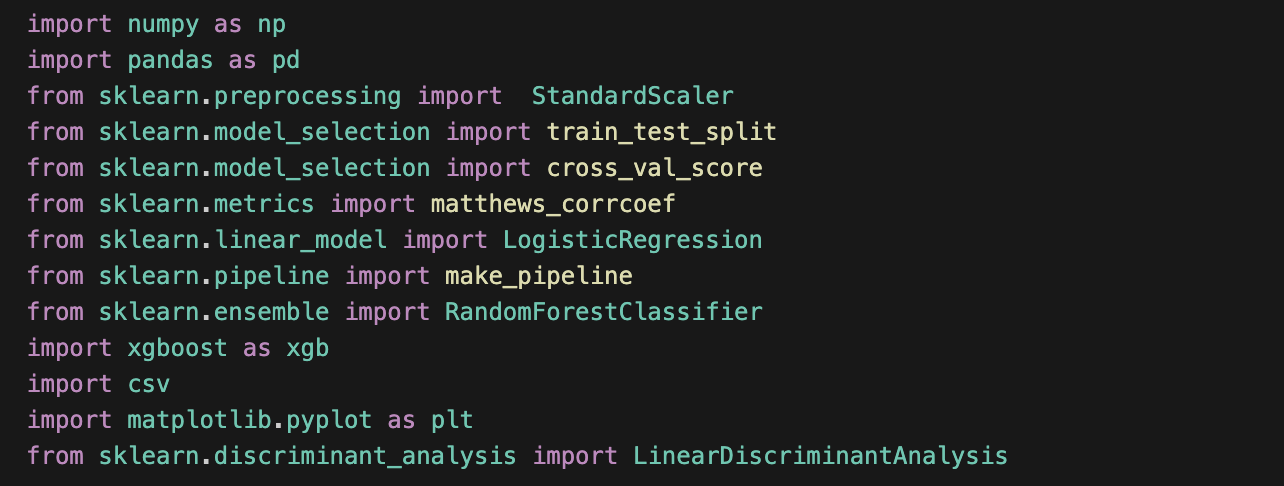
\includegraphics[width=1\linewidth]{1.png}
    \label{fig:enter-label}
\end{figure}

\begin{figure}[H]
    \centering
    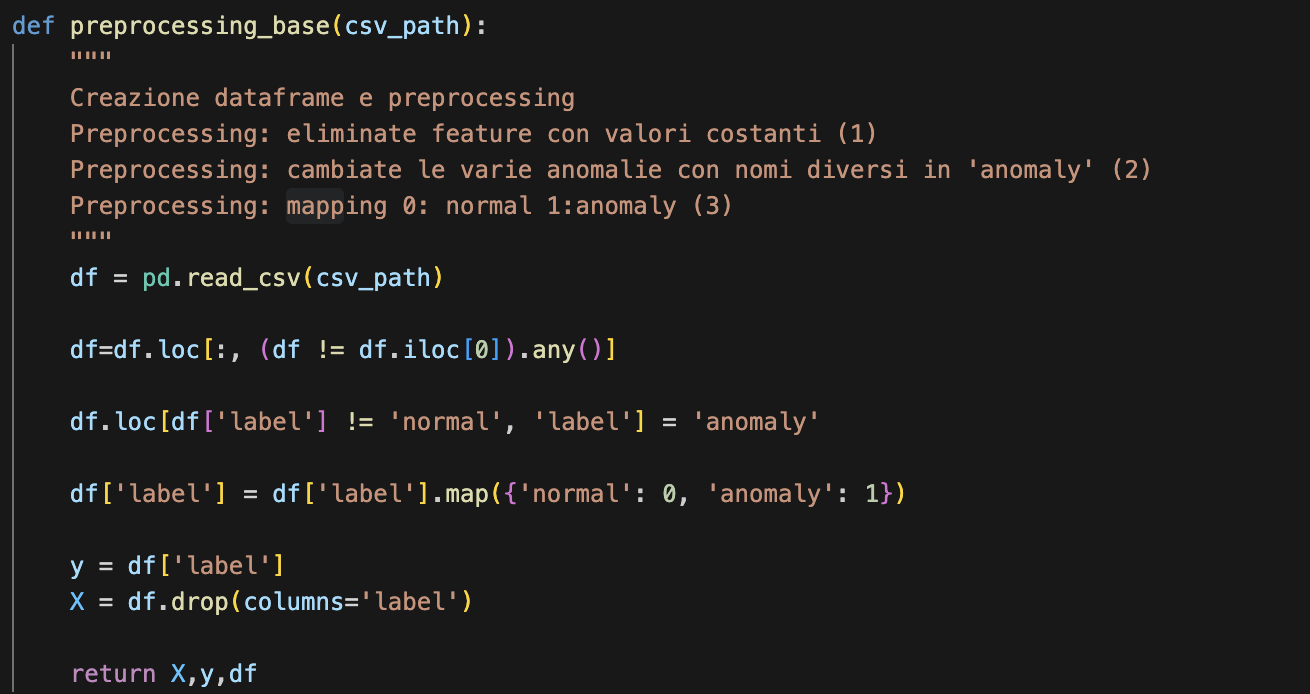
\includegraphics[width=1\linewidth]{2.png}
    \label{fig:enter-label}
\end{figure}

\begin{figure}[H]
    \centering
    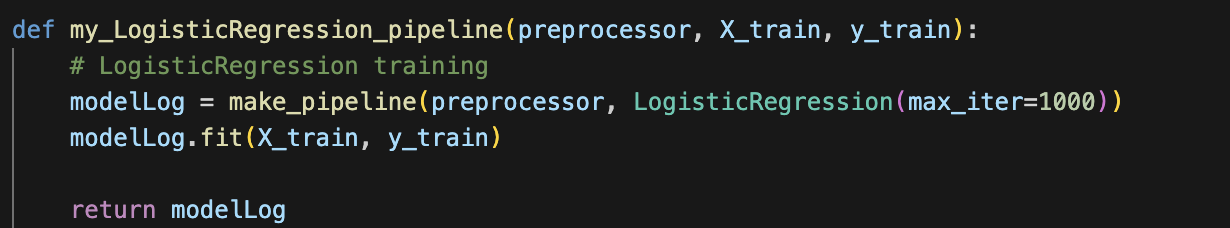
\includegraphics[width=1\linewidth]{3.png}
    \label{fig:enter-label}
\end{figure}

\begin{figure}[H]
    \centering
    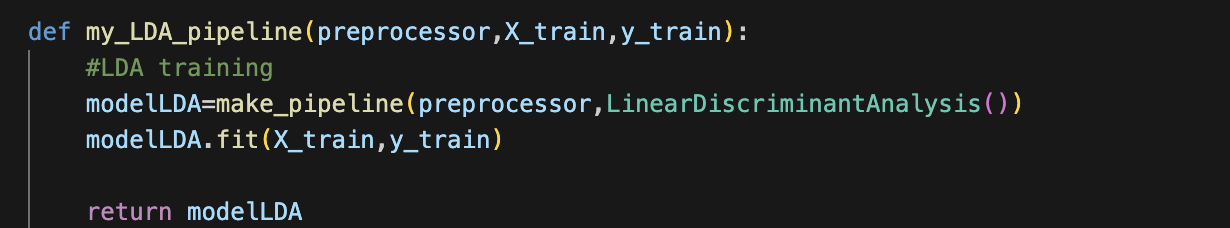
\includegraphics[width=1\linewidth]{4.png}
    \label{fig:enter-label}
\end{figure}

\begin{figure}[H]
    \centering
    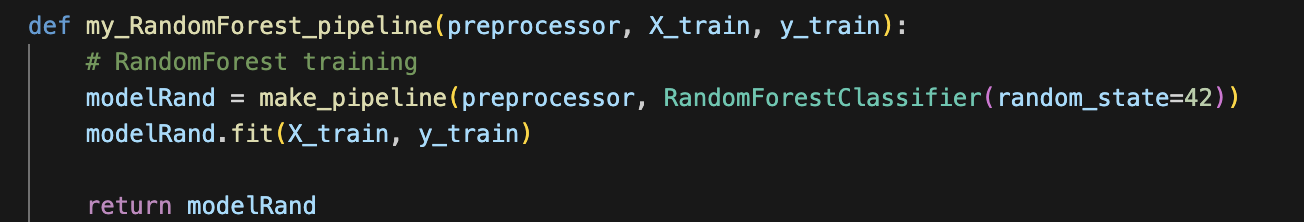
\includegraphics[width=1\linewidth]{5.png}
    \label{fig:enter-label}
\end{figure}

\begin{figure}[H]
    \centering
    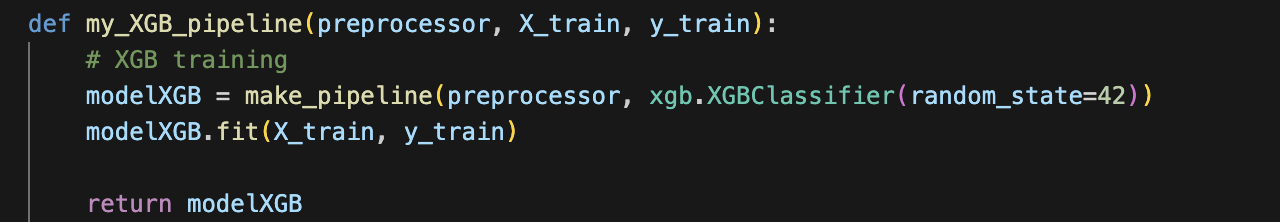
\includegraphics[width=1\linewidth]{6.png}
    \label{fig:enter-label}
\end{figure}

\begin{figure}[H]
    \centering
    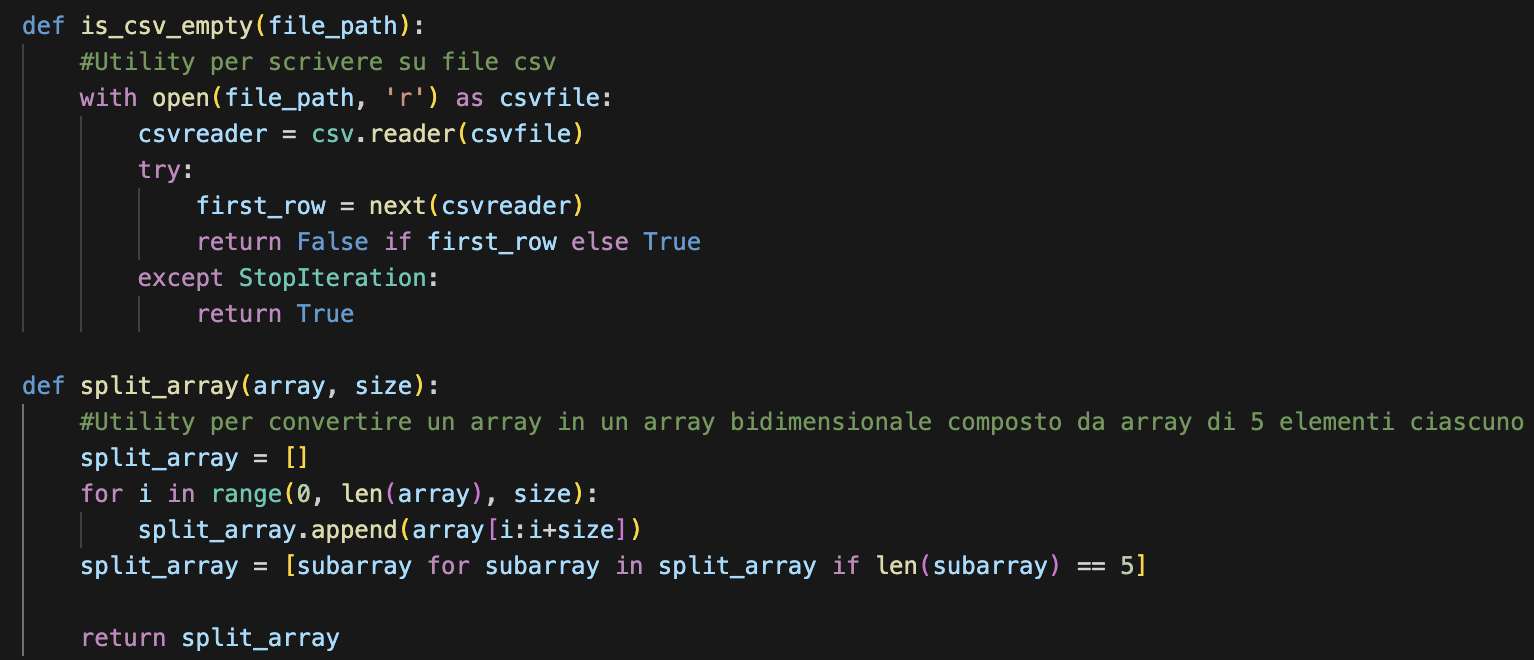
\includegraphics[width=1\linewidth]{7.png}
    \label{fig:enter-label}
\end{figure}

\begin{figure}[H]
    \centering
    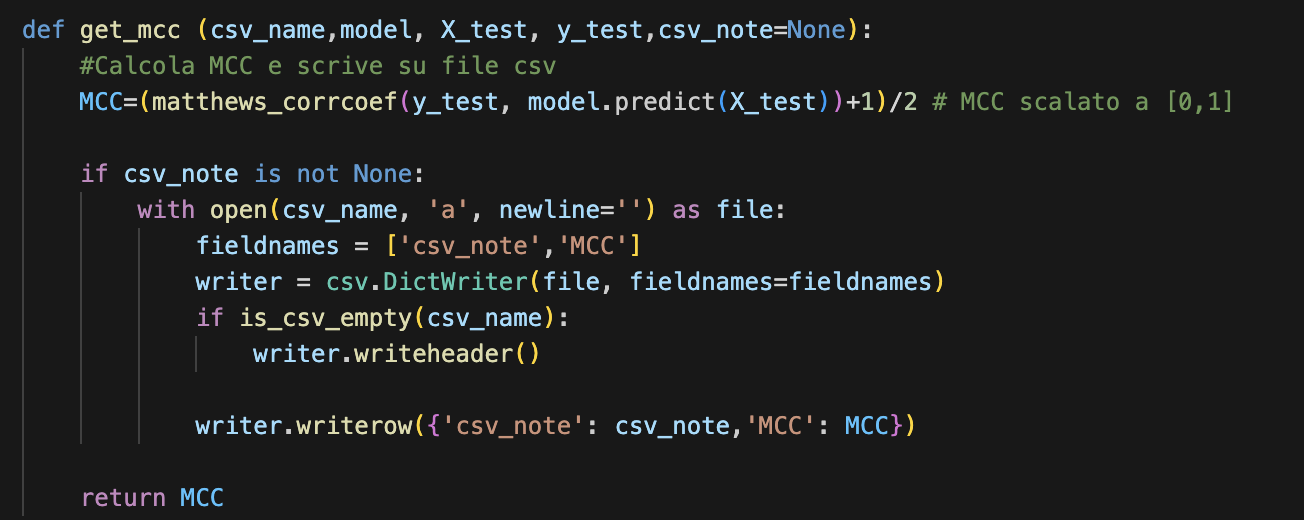
\includegraphics[width=1\linewidth]{8.png}
    \label{fig:enter-label}
\end{figure}

\begin{figure}[H]
    \centering
    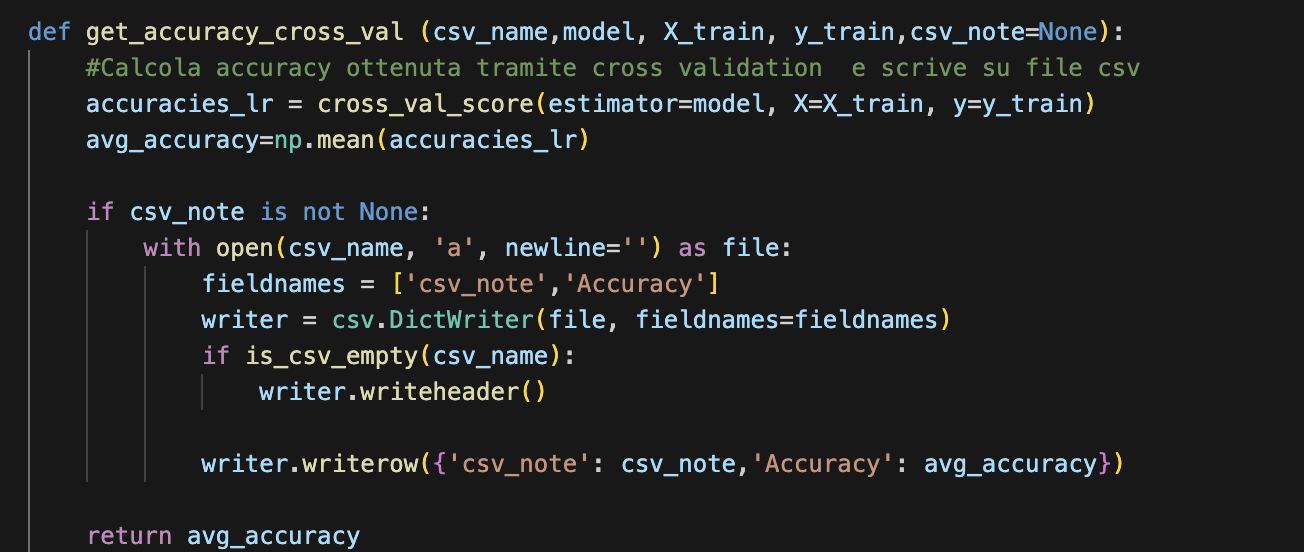
\includegraphics[width=1\linewidth]{9.png}
    \label{fig:enter-label}
\end{figure}

\begin{figure}[H]
    \centering
    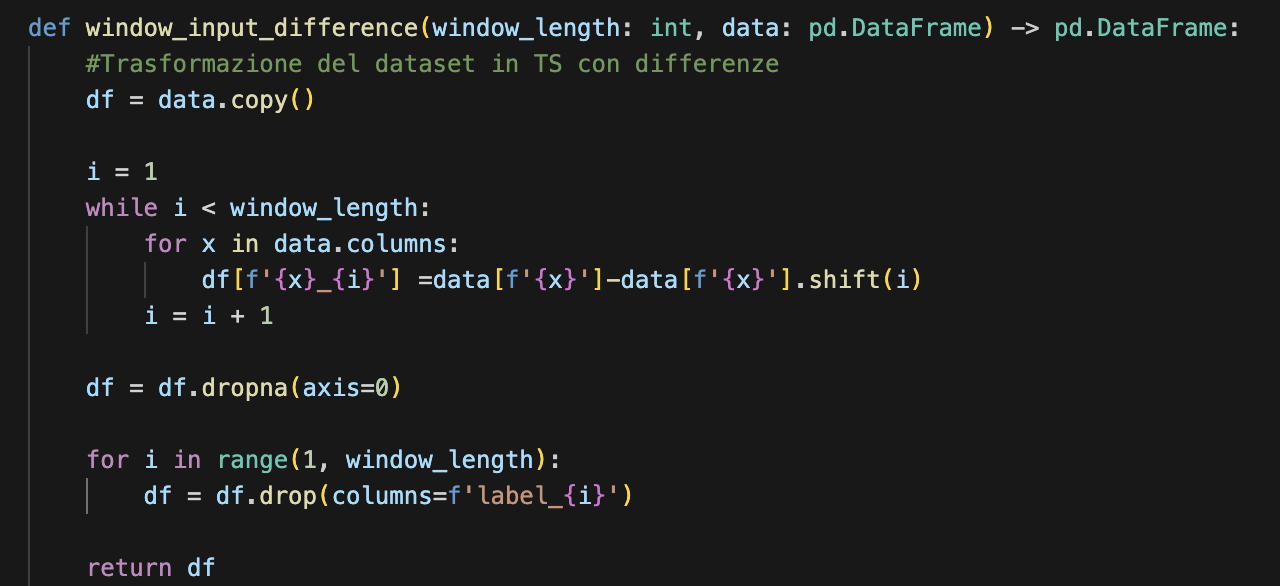
\includegraphics[width=1\linewidth]{10.png}
    \label{fig:enter-label}
\end{figure}

\begin{figure}[H]
    \centering
    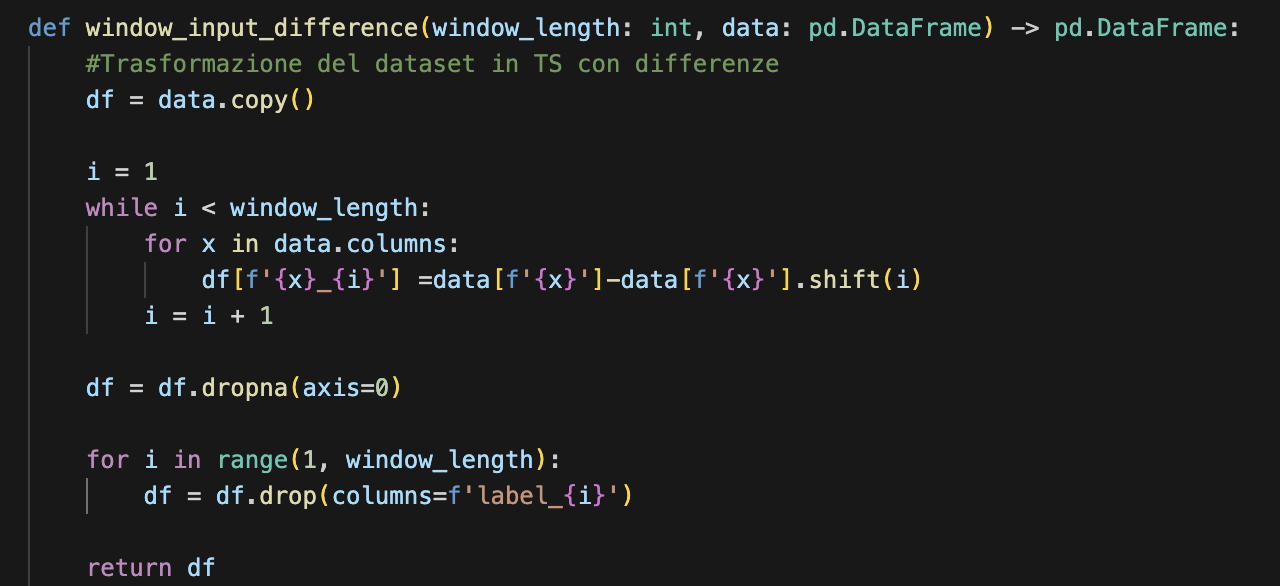
\includegraphics[width=1\linewidth]{10.png}
    \label{fig:enter-label}
\end{figure}

\begin{figure}[H]
    \centering
    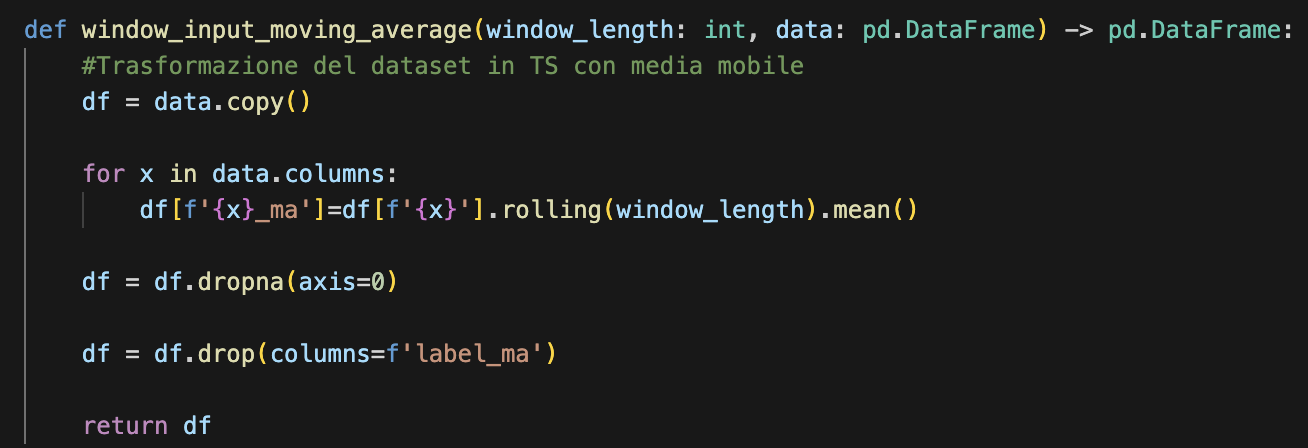
\includegraphics[width=1\linewidth]{11.png}
    \label{fig:enter-label}
\end{figure}

\begin{figure}[H]
    \centering
    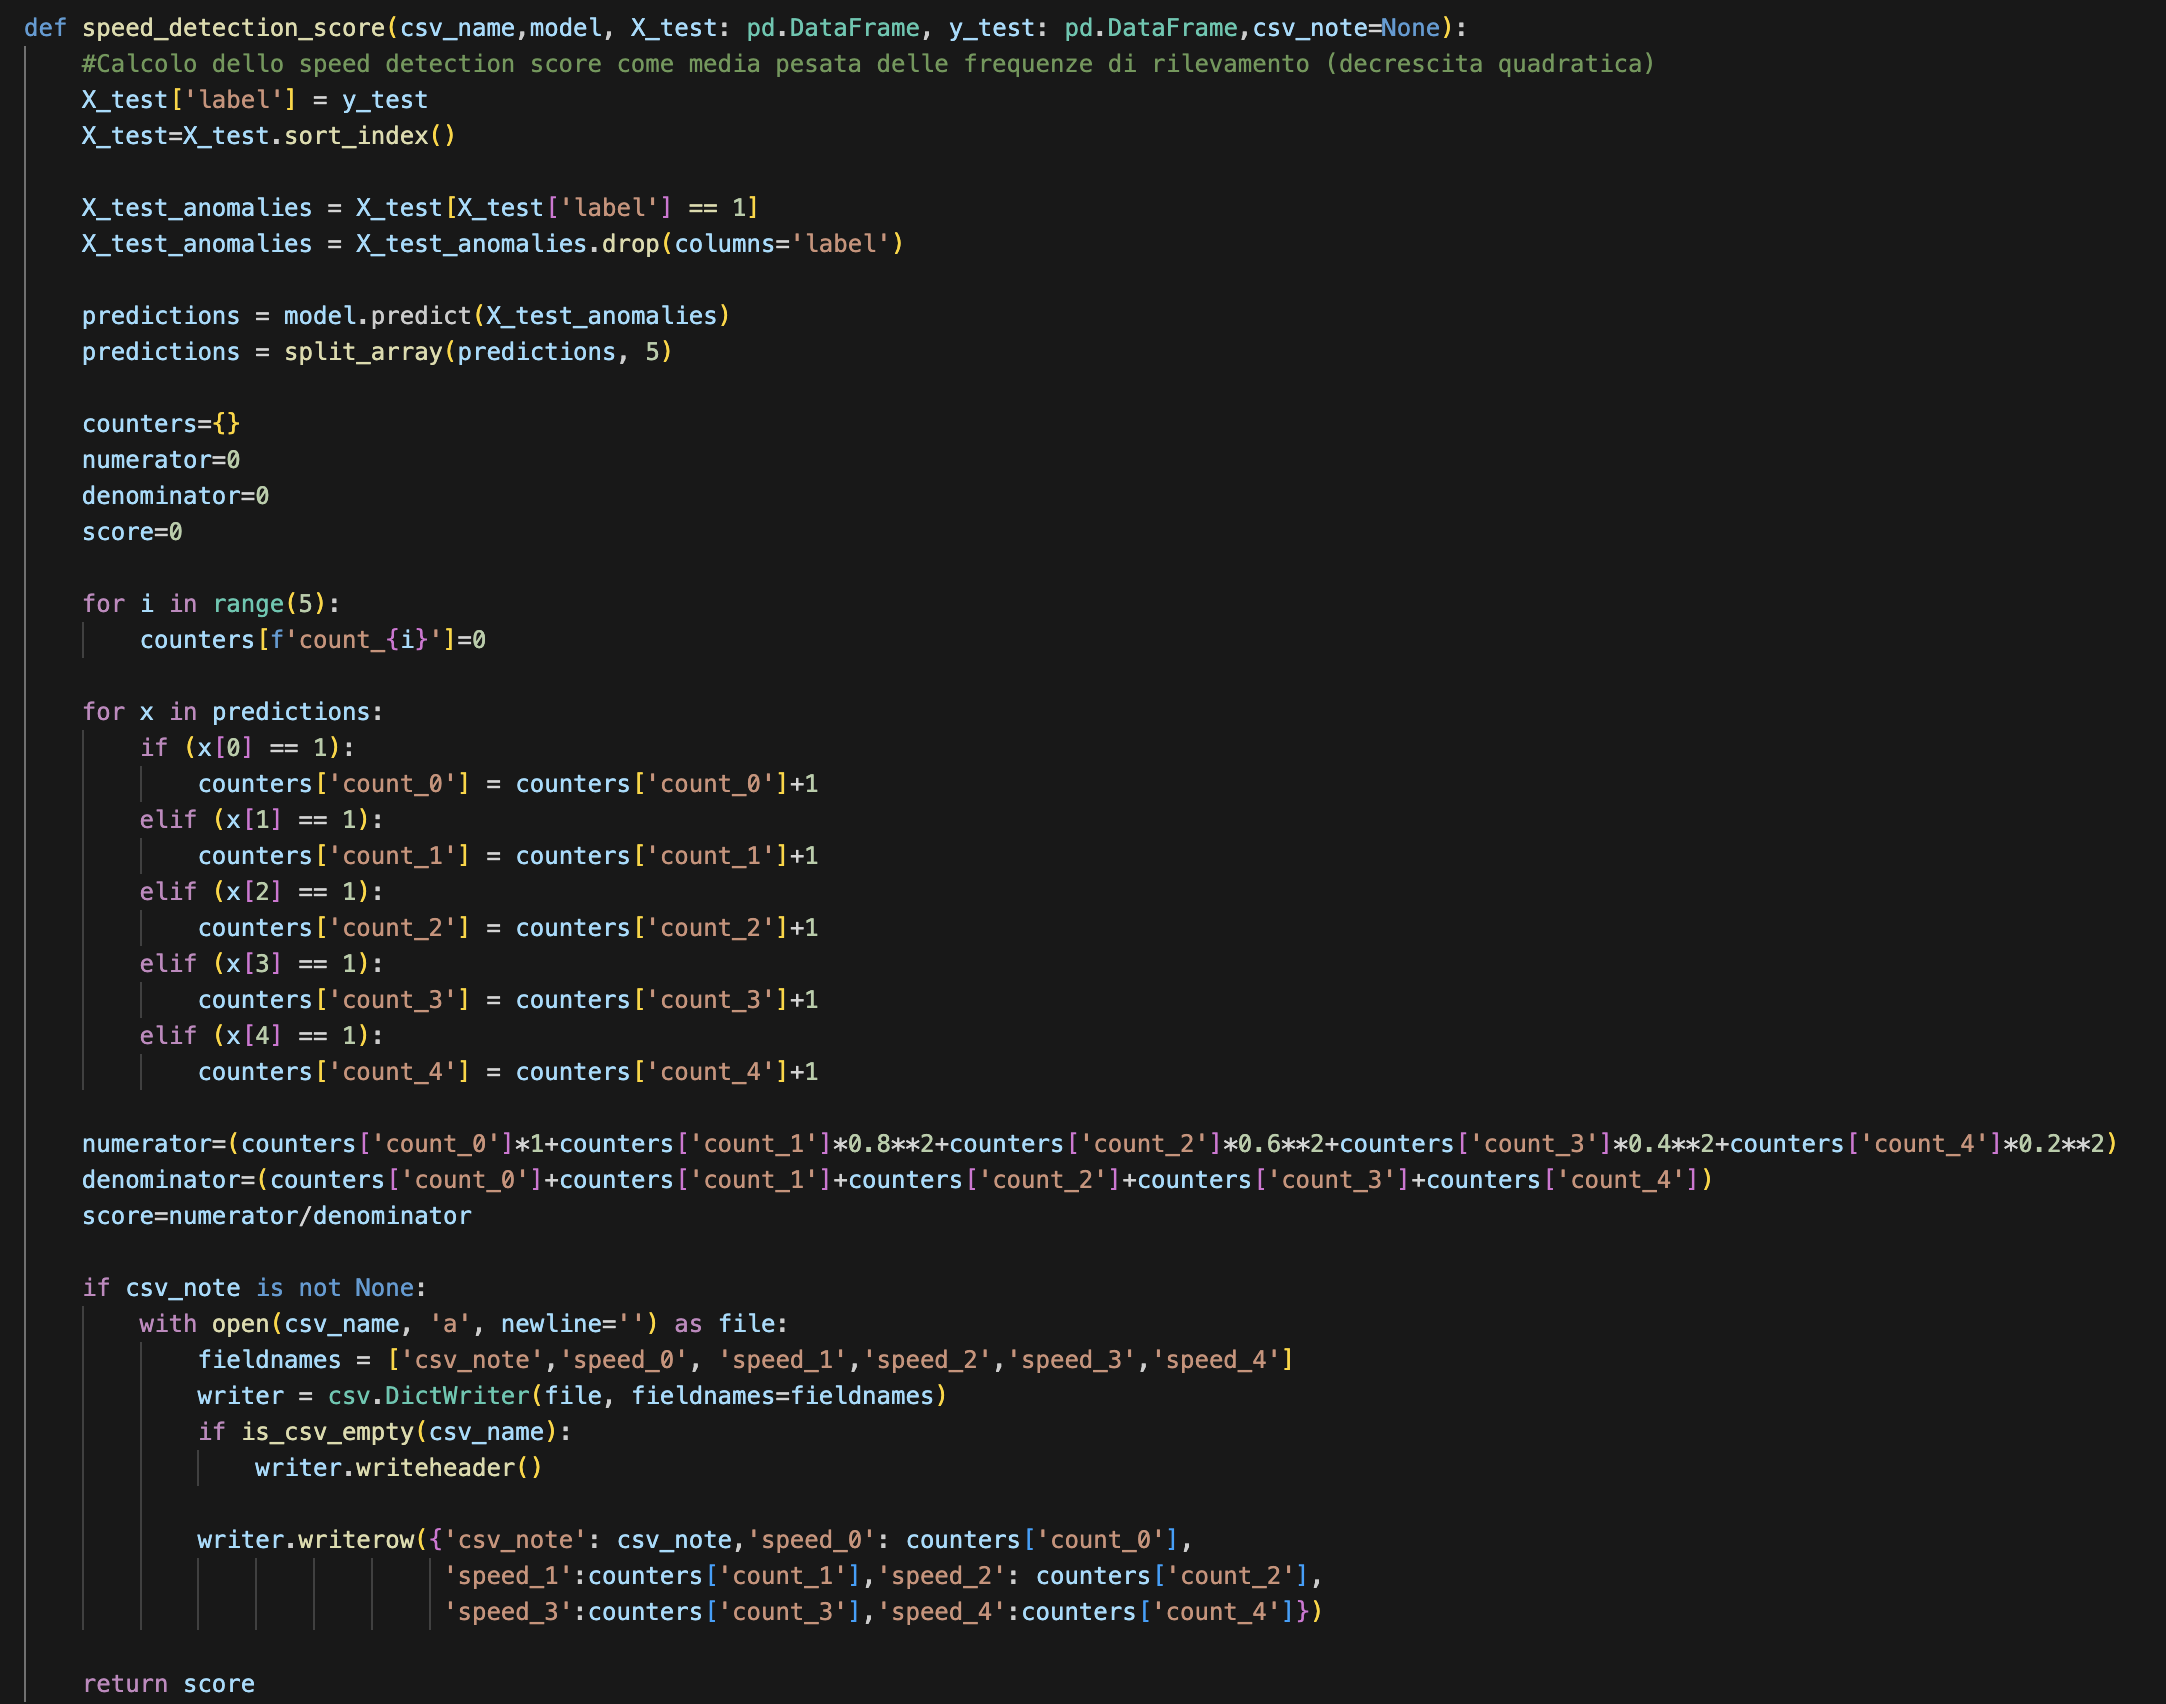
\includegraphics[width=1\linewidth]{12.png}
    \label{fig:enter-label}
\end{figure}

\begin{figure}[H]
    \centering
    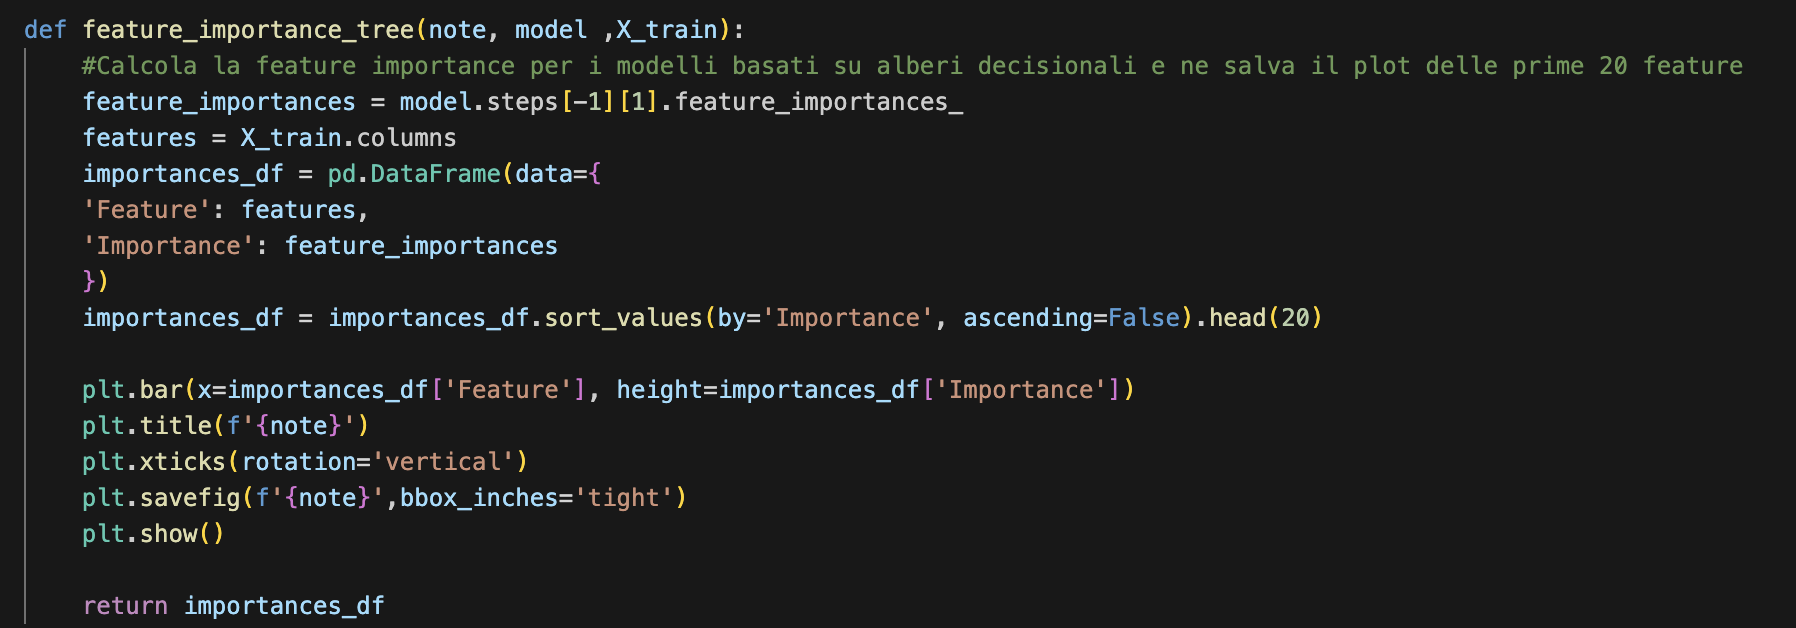
\includegraphics[width=1\linewidth]{13.png}
    \label{fig:enter-label}
\end{figure}

\begin{figure}[H]
    \centering
    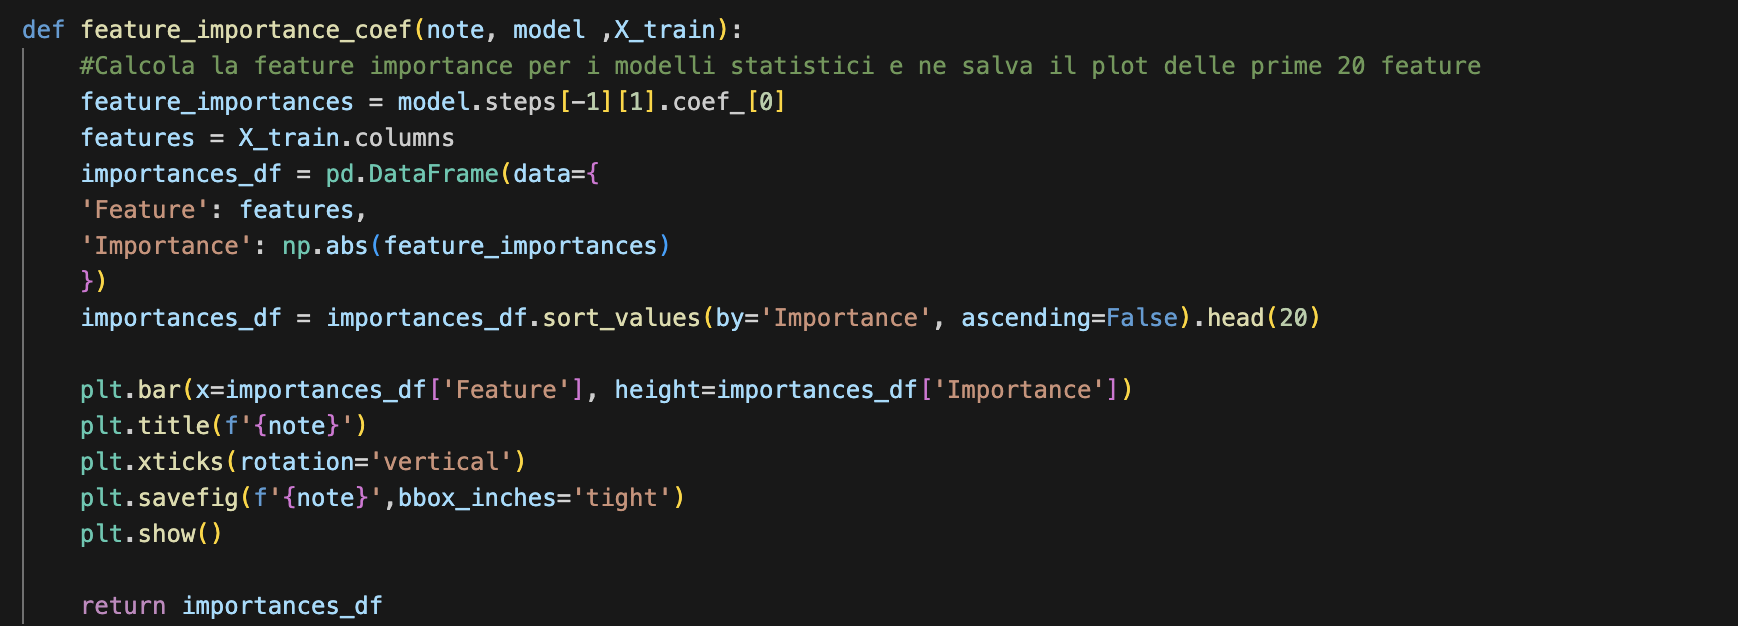
\includegraphics[width=1\linewidth]{14.png}
    \label{fig:enter-label}
\end{figure}

\begin{figure}[H]
    \centering
    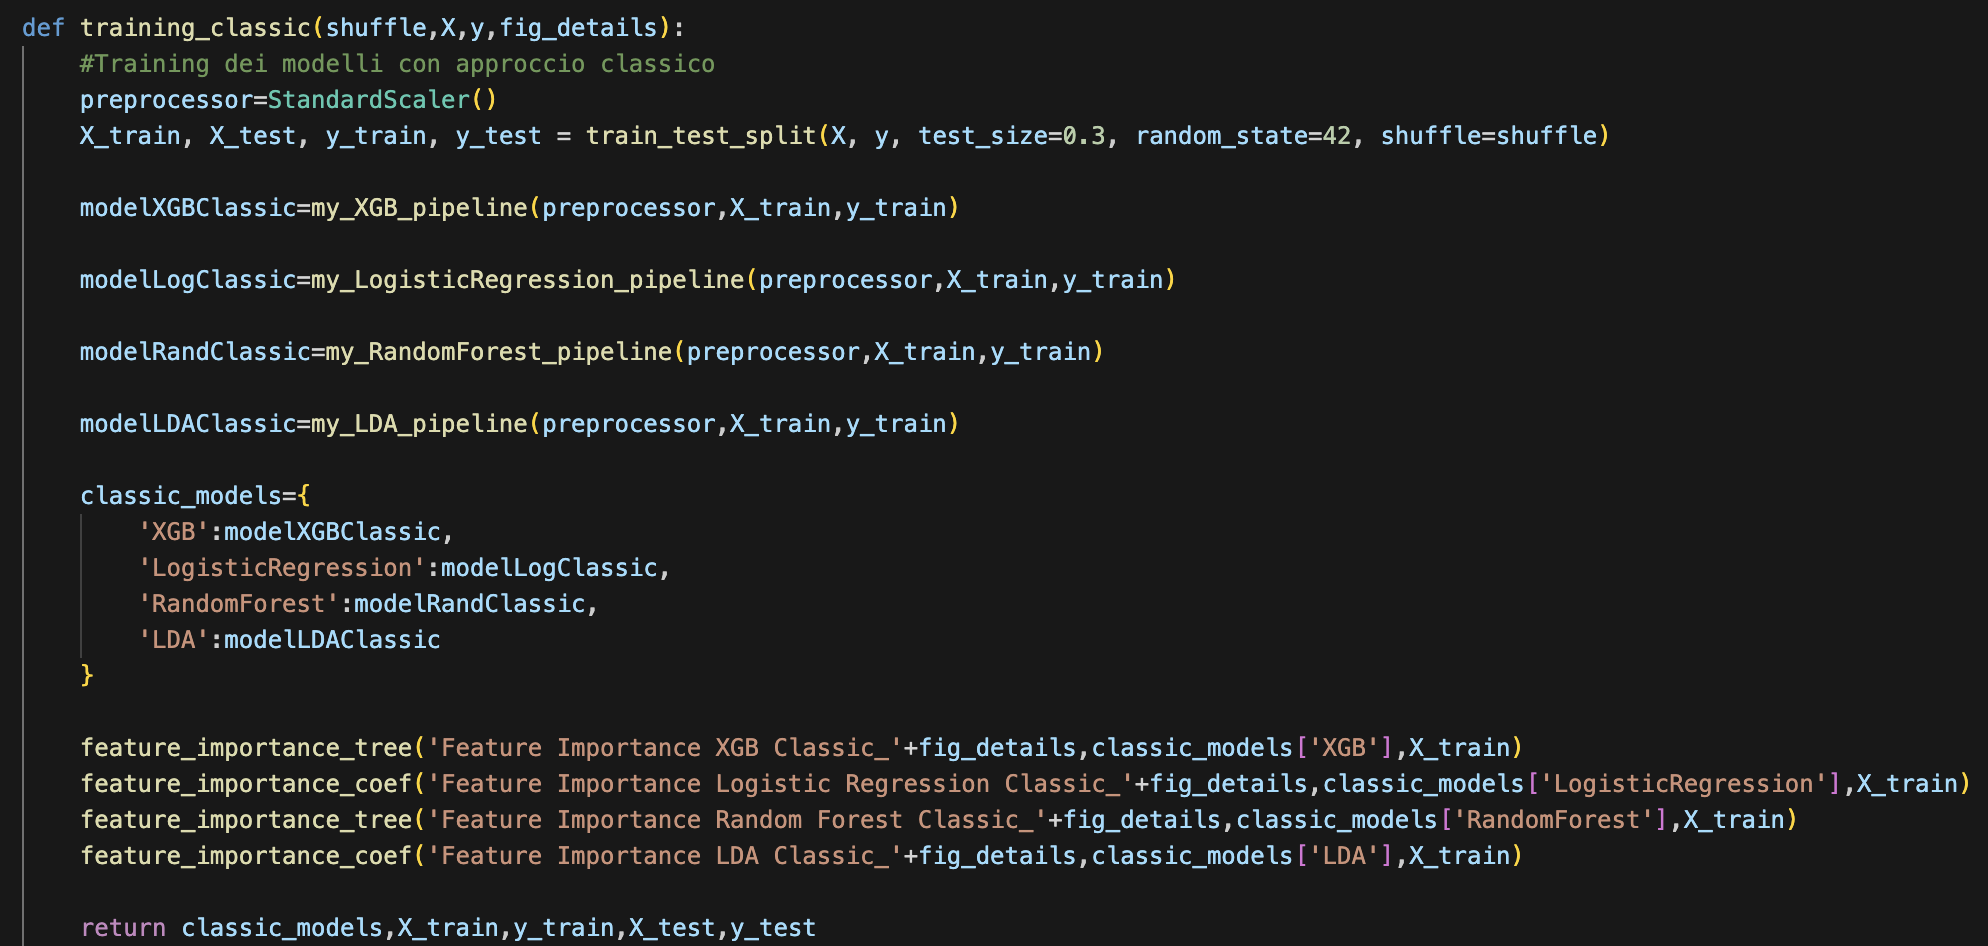
\includegraphics[width=1\linewidth]{15.png}
    \label{fig:enter-label}
\end{figure}

\begin{figure}[H]
    \centering
    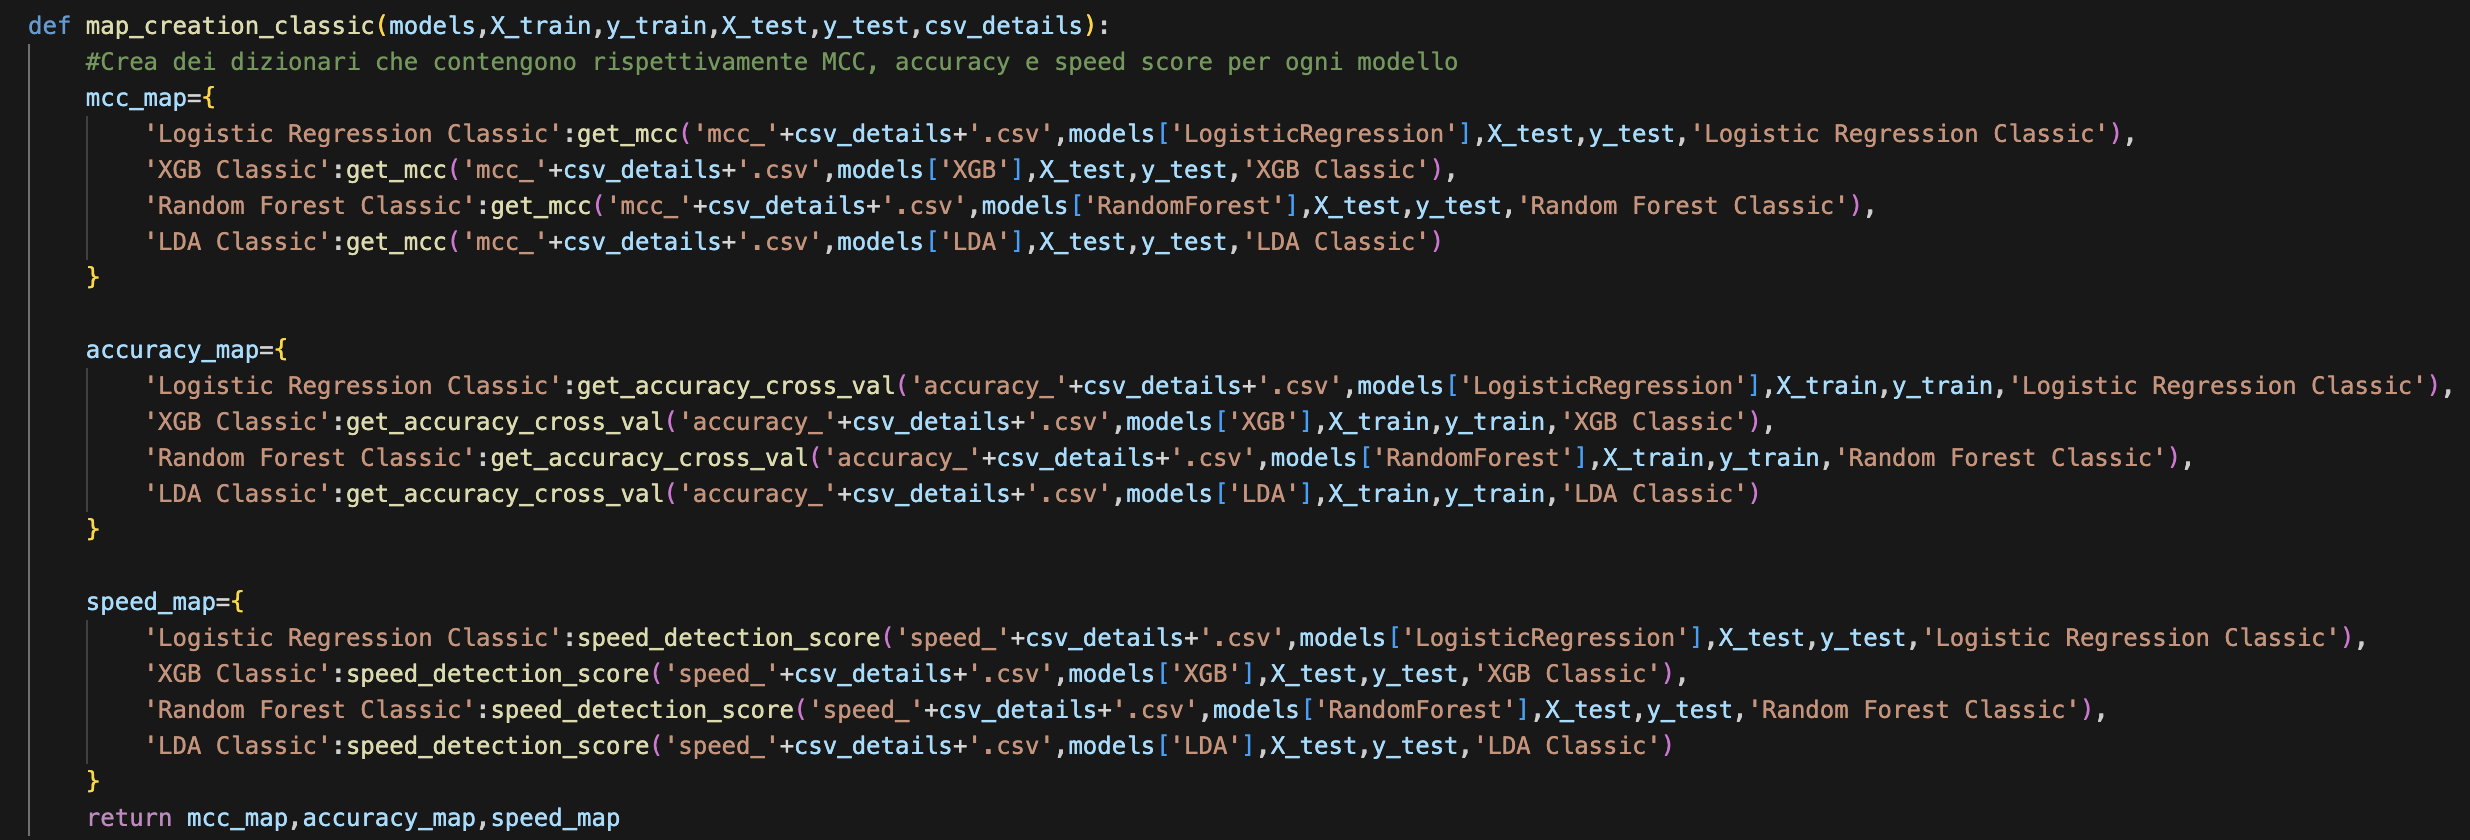
\includegraphics[width=1\linewidth]{16.png}
    \label{fig:enter-label}
\end{figure}

\begin{figure}[H]
    \centering
    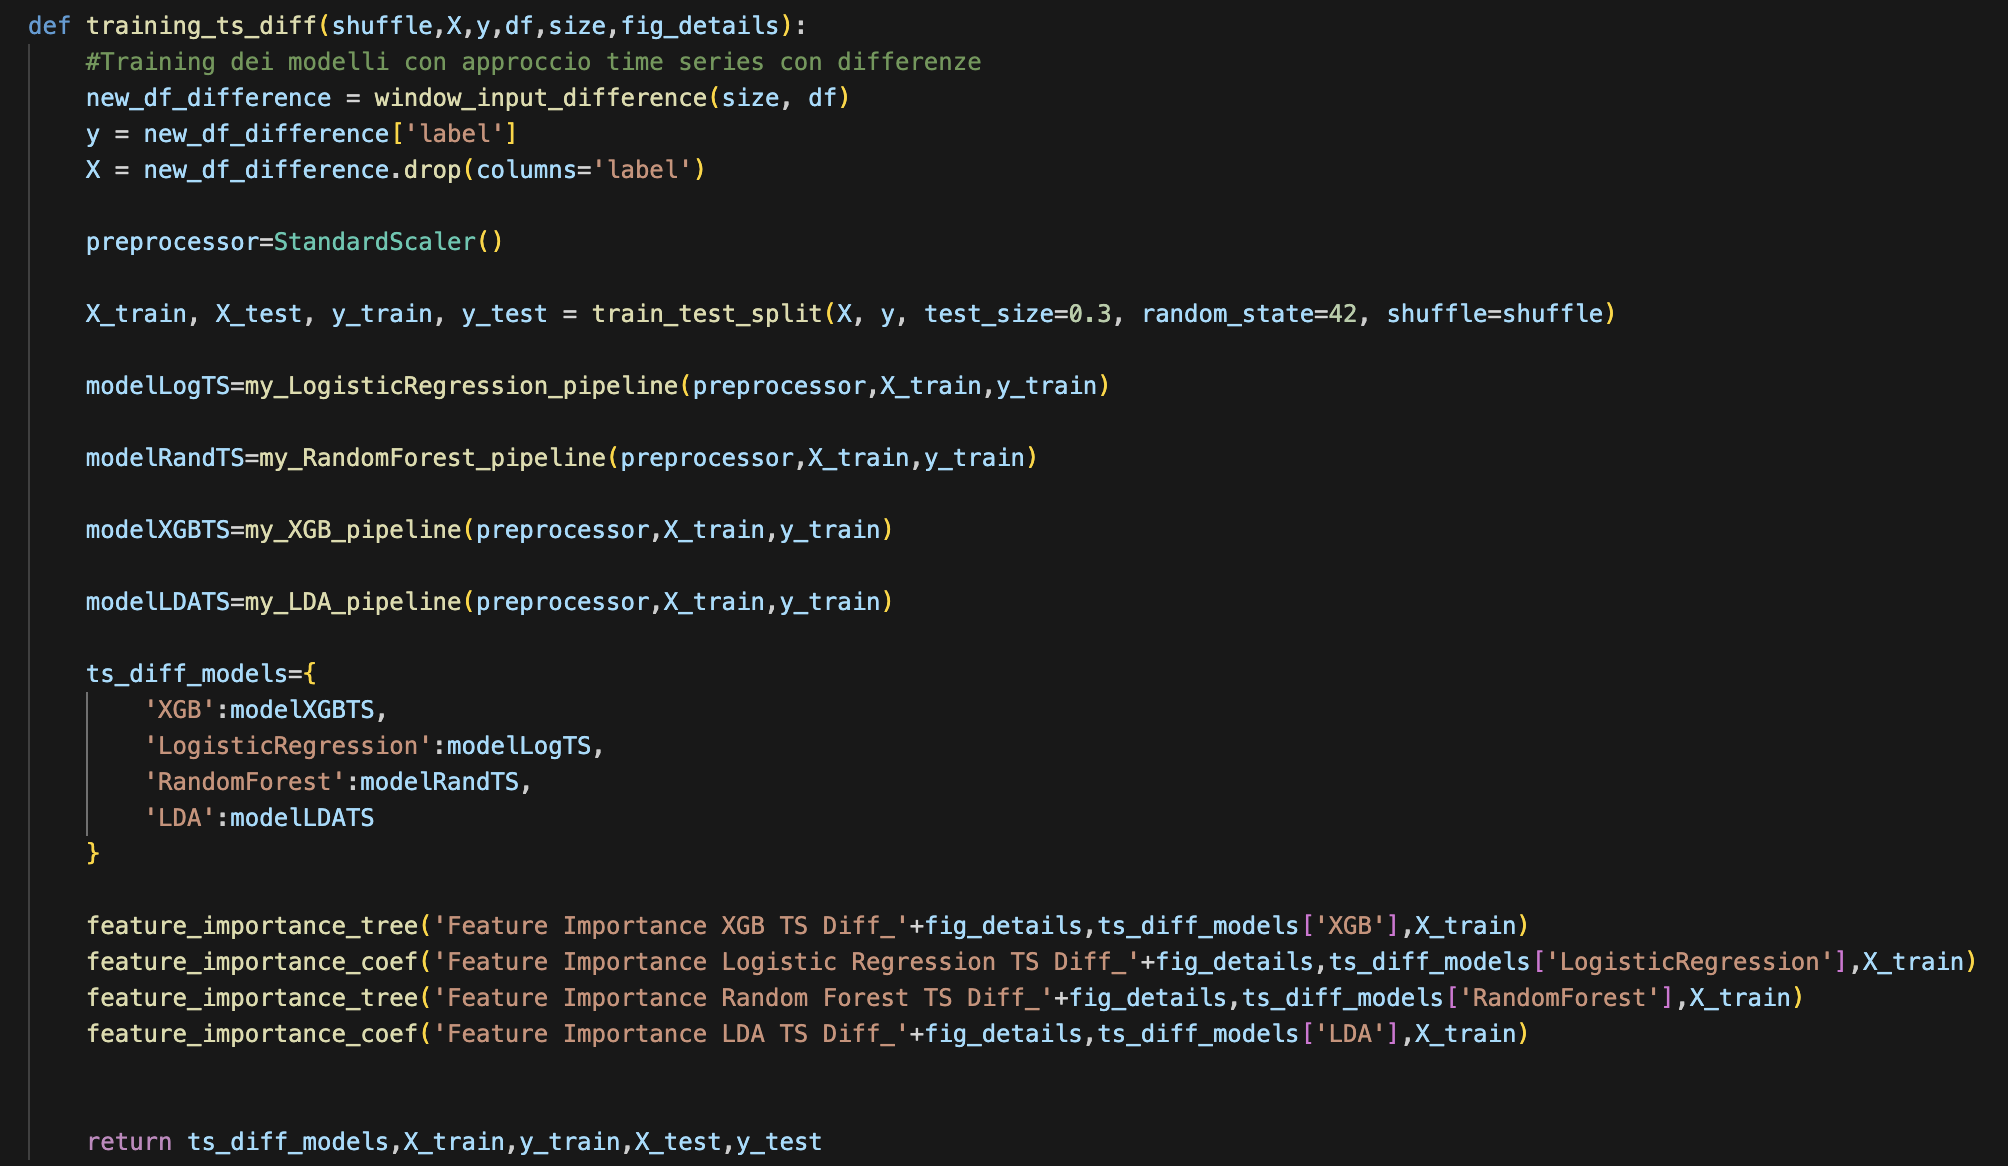
\includegraphics[width=1\linewidth]{17.png}
    \label{fig:enter-label}
\end{figure}

\begin{figure}[H]
    \centering
    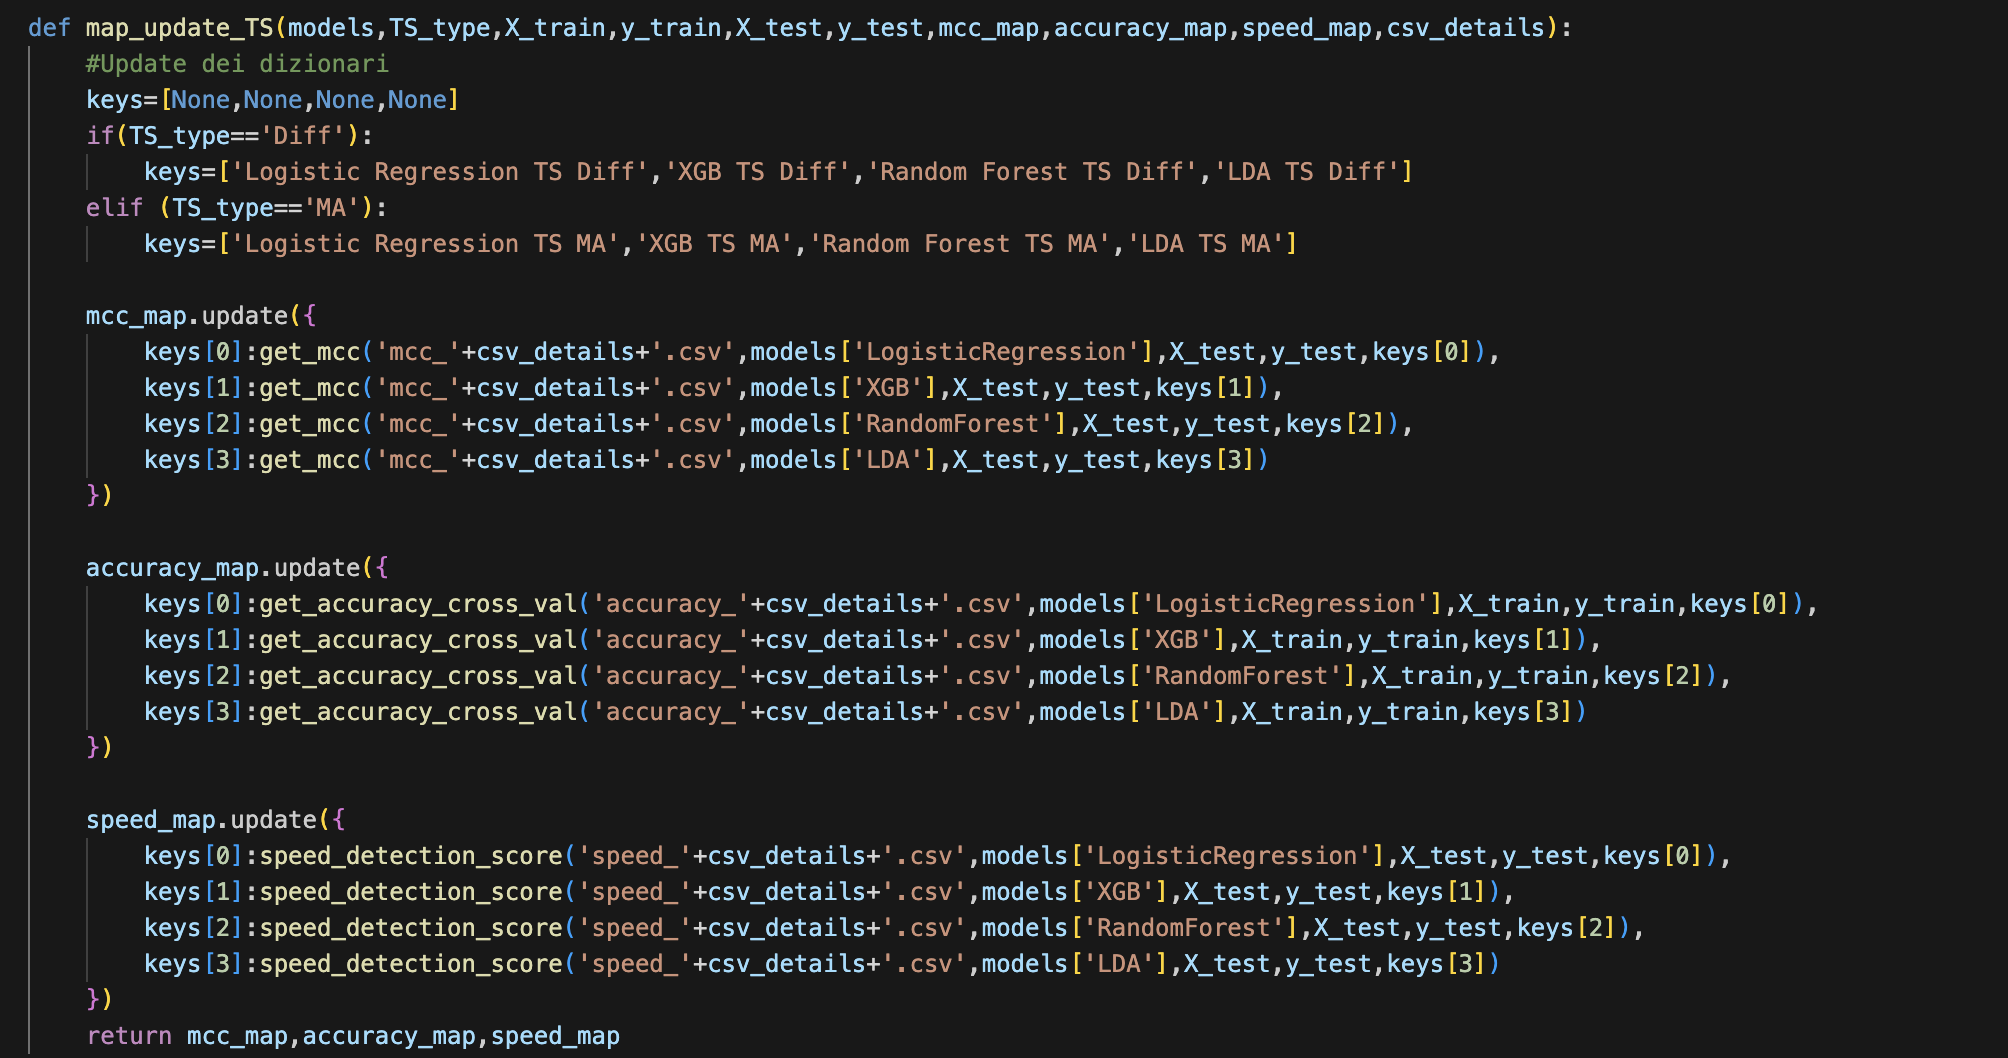
\includegraphics[width=1\linewidth]{18.png}
    \label{fig:enter-label}
\end{figure}

\begin{figure}[H]
    \centering
    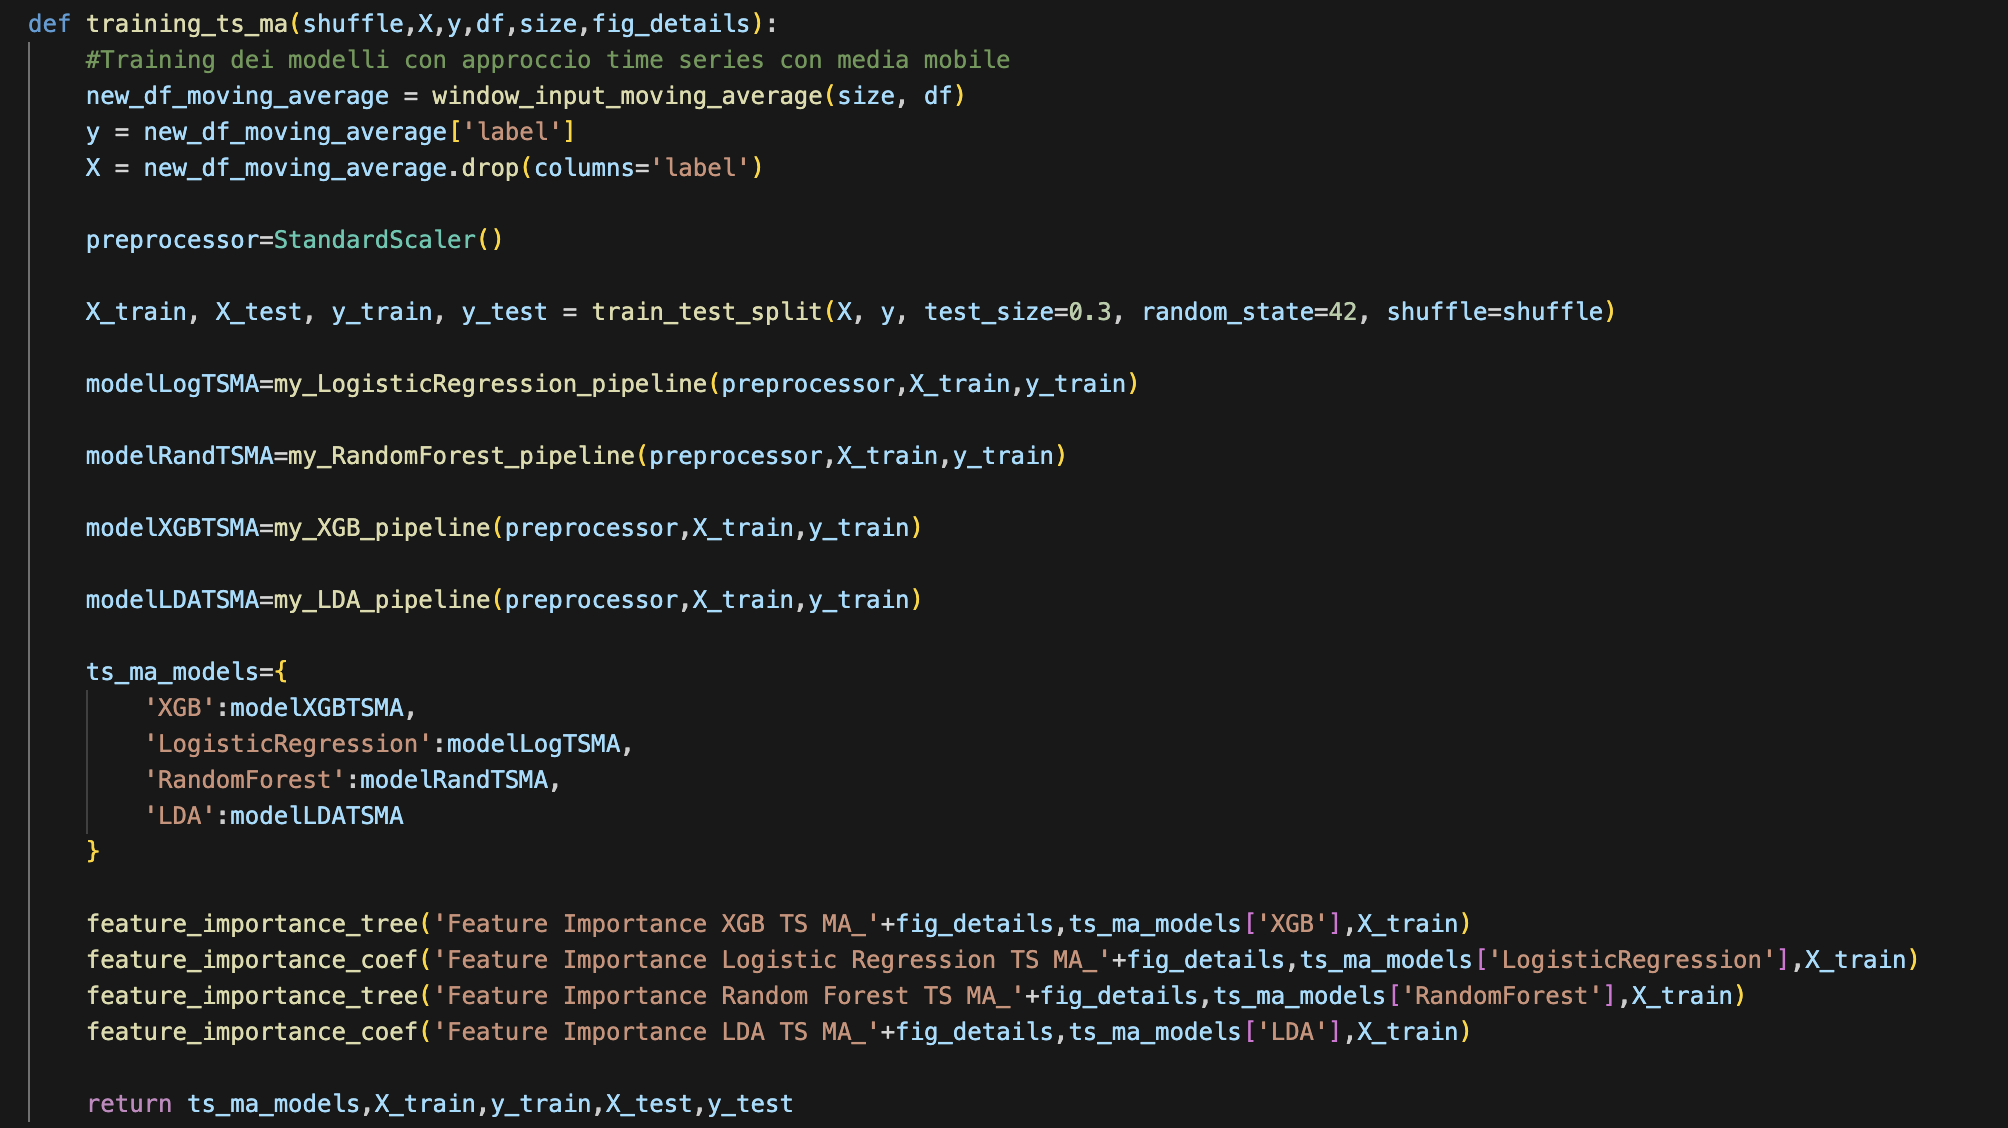
\includegraphics[width=1\linewidth]{19.png}
    \label{fig:enter-label}
\end{figure}

\begin{figure}[H]
    \centering
    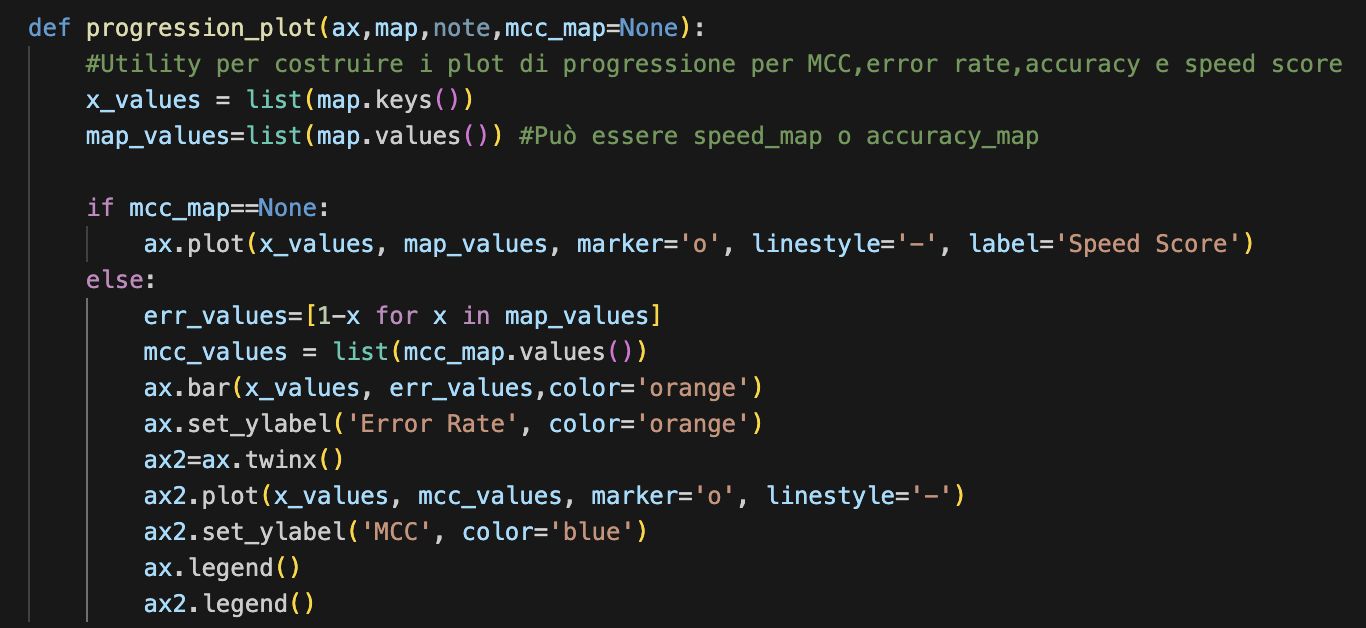
\includegraphics[width=1\linewidth]{20.png}
    \label{fig:enter-label}
\end{figure}

\begin{figure}[H]
    \centering
    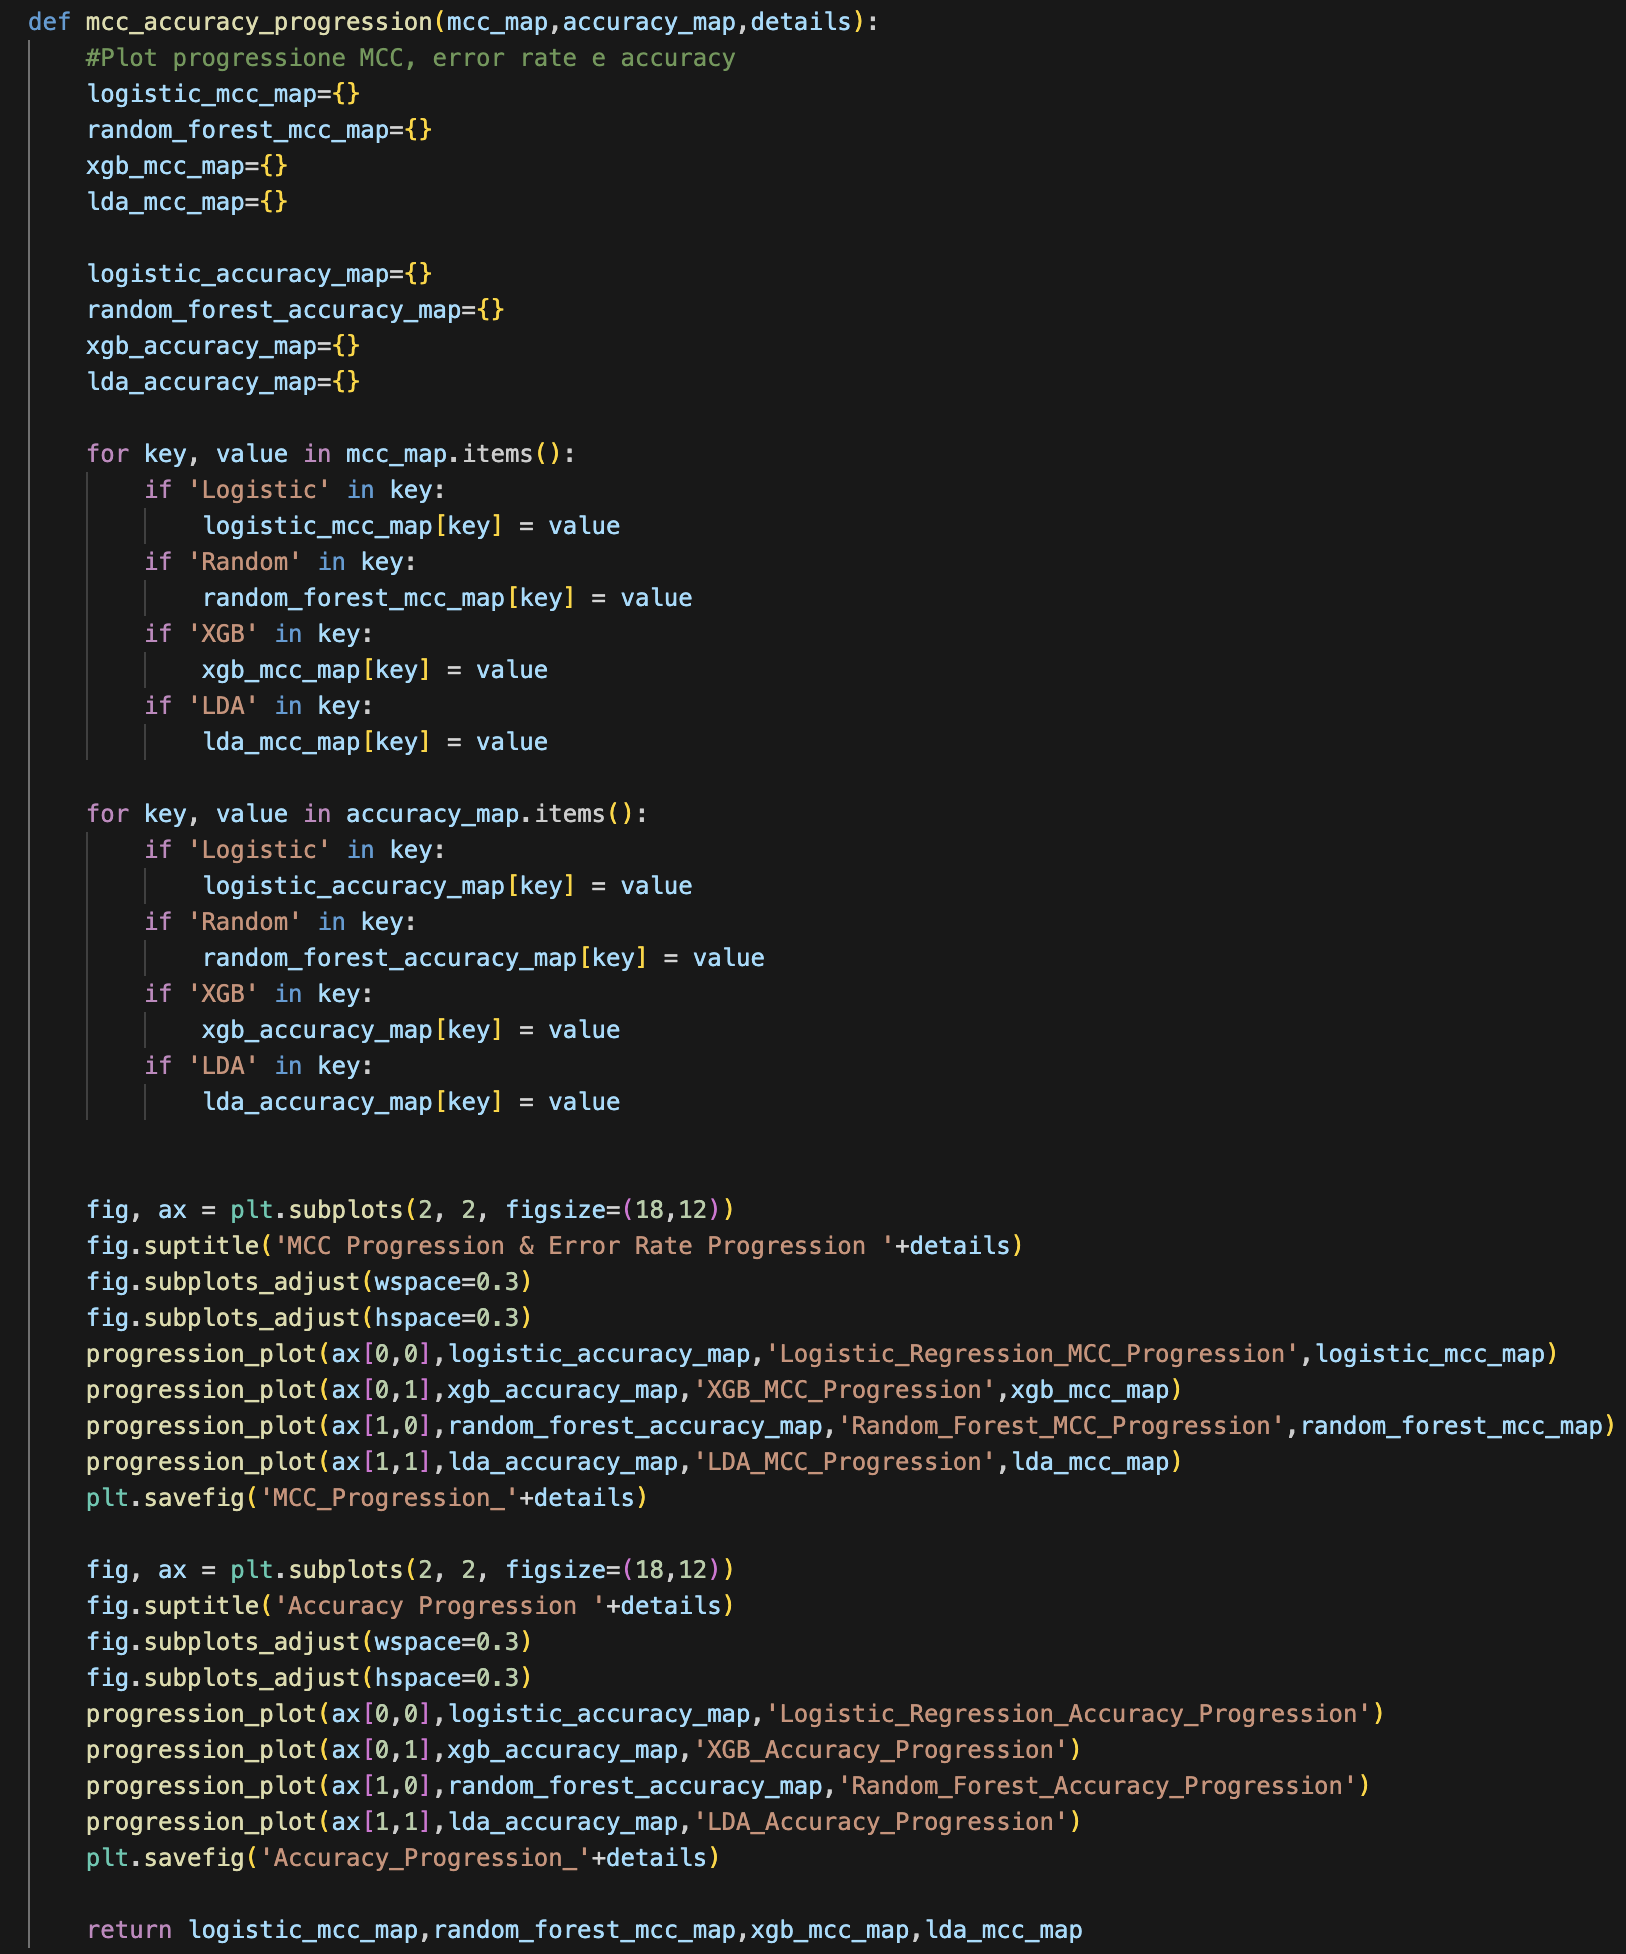
\includegraphics[width=1\linewidth]{21.png}
    \label{fig:enter-label}
\end{figure}

\begin{figure}[H]
    \centering
    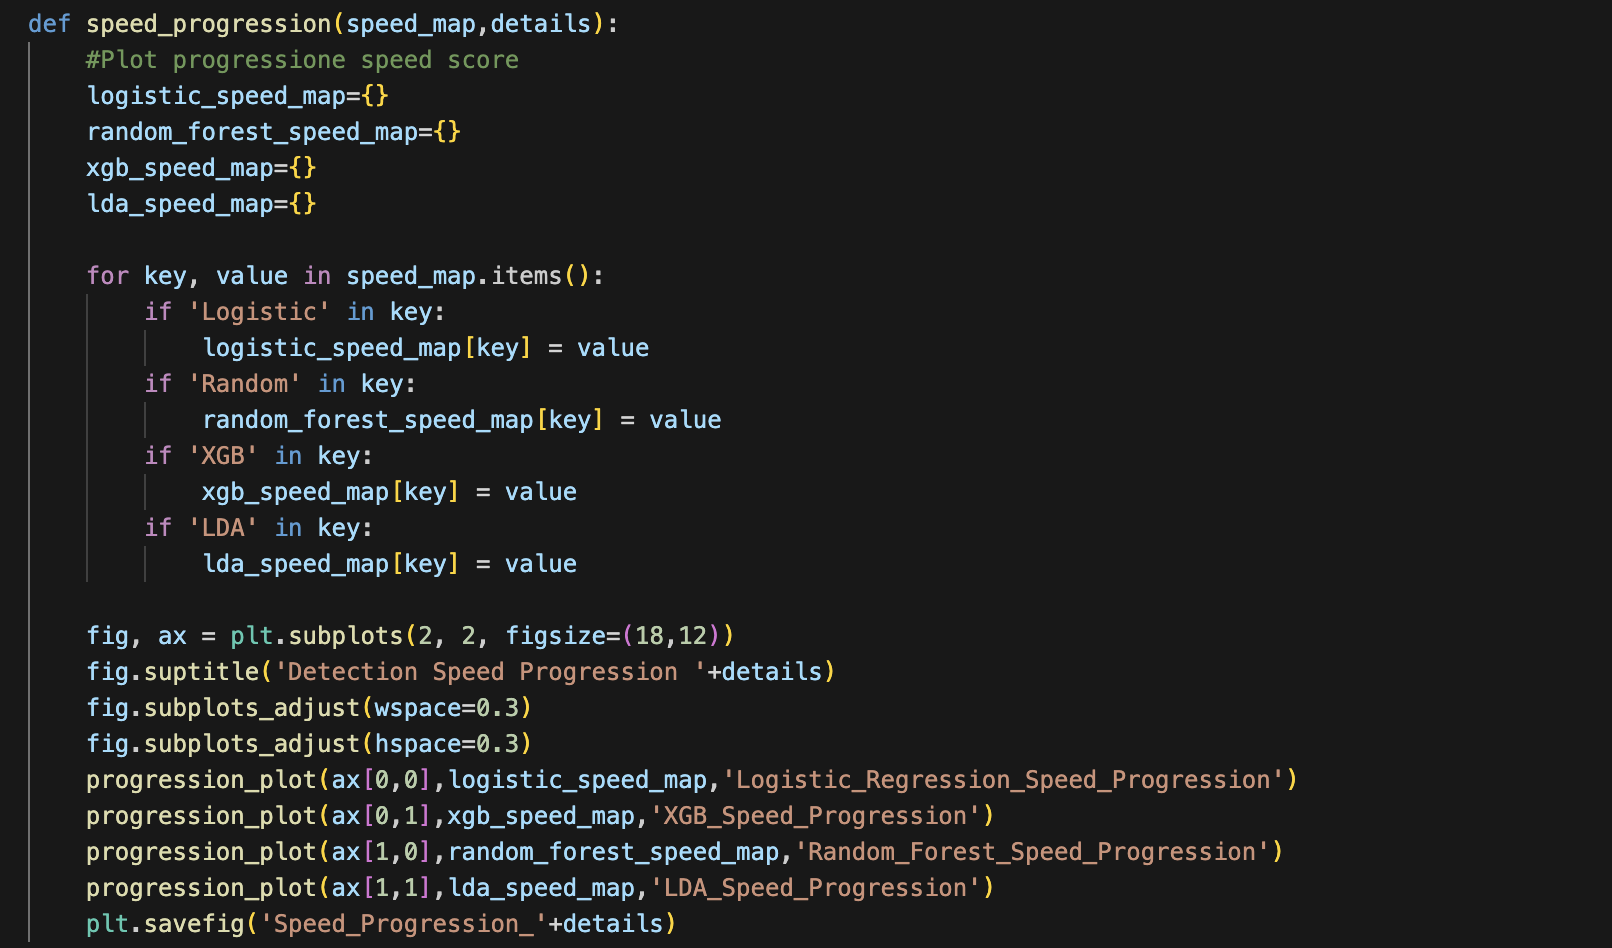
\includegraphics[width=1\linewidth]{22.png}
    \label{fig:enter-label}
\end{figure}

\begin{figure}[H]
    \centering
    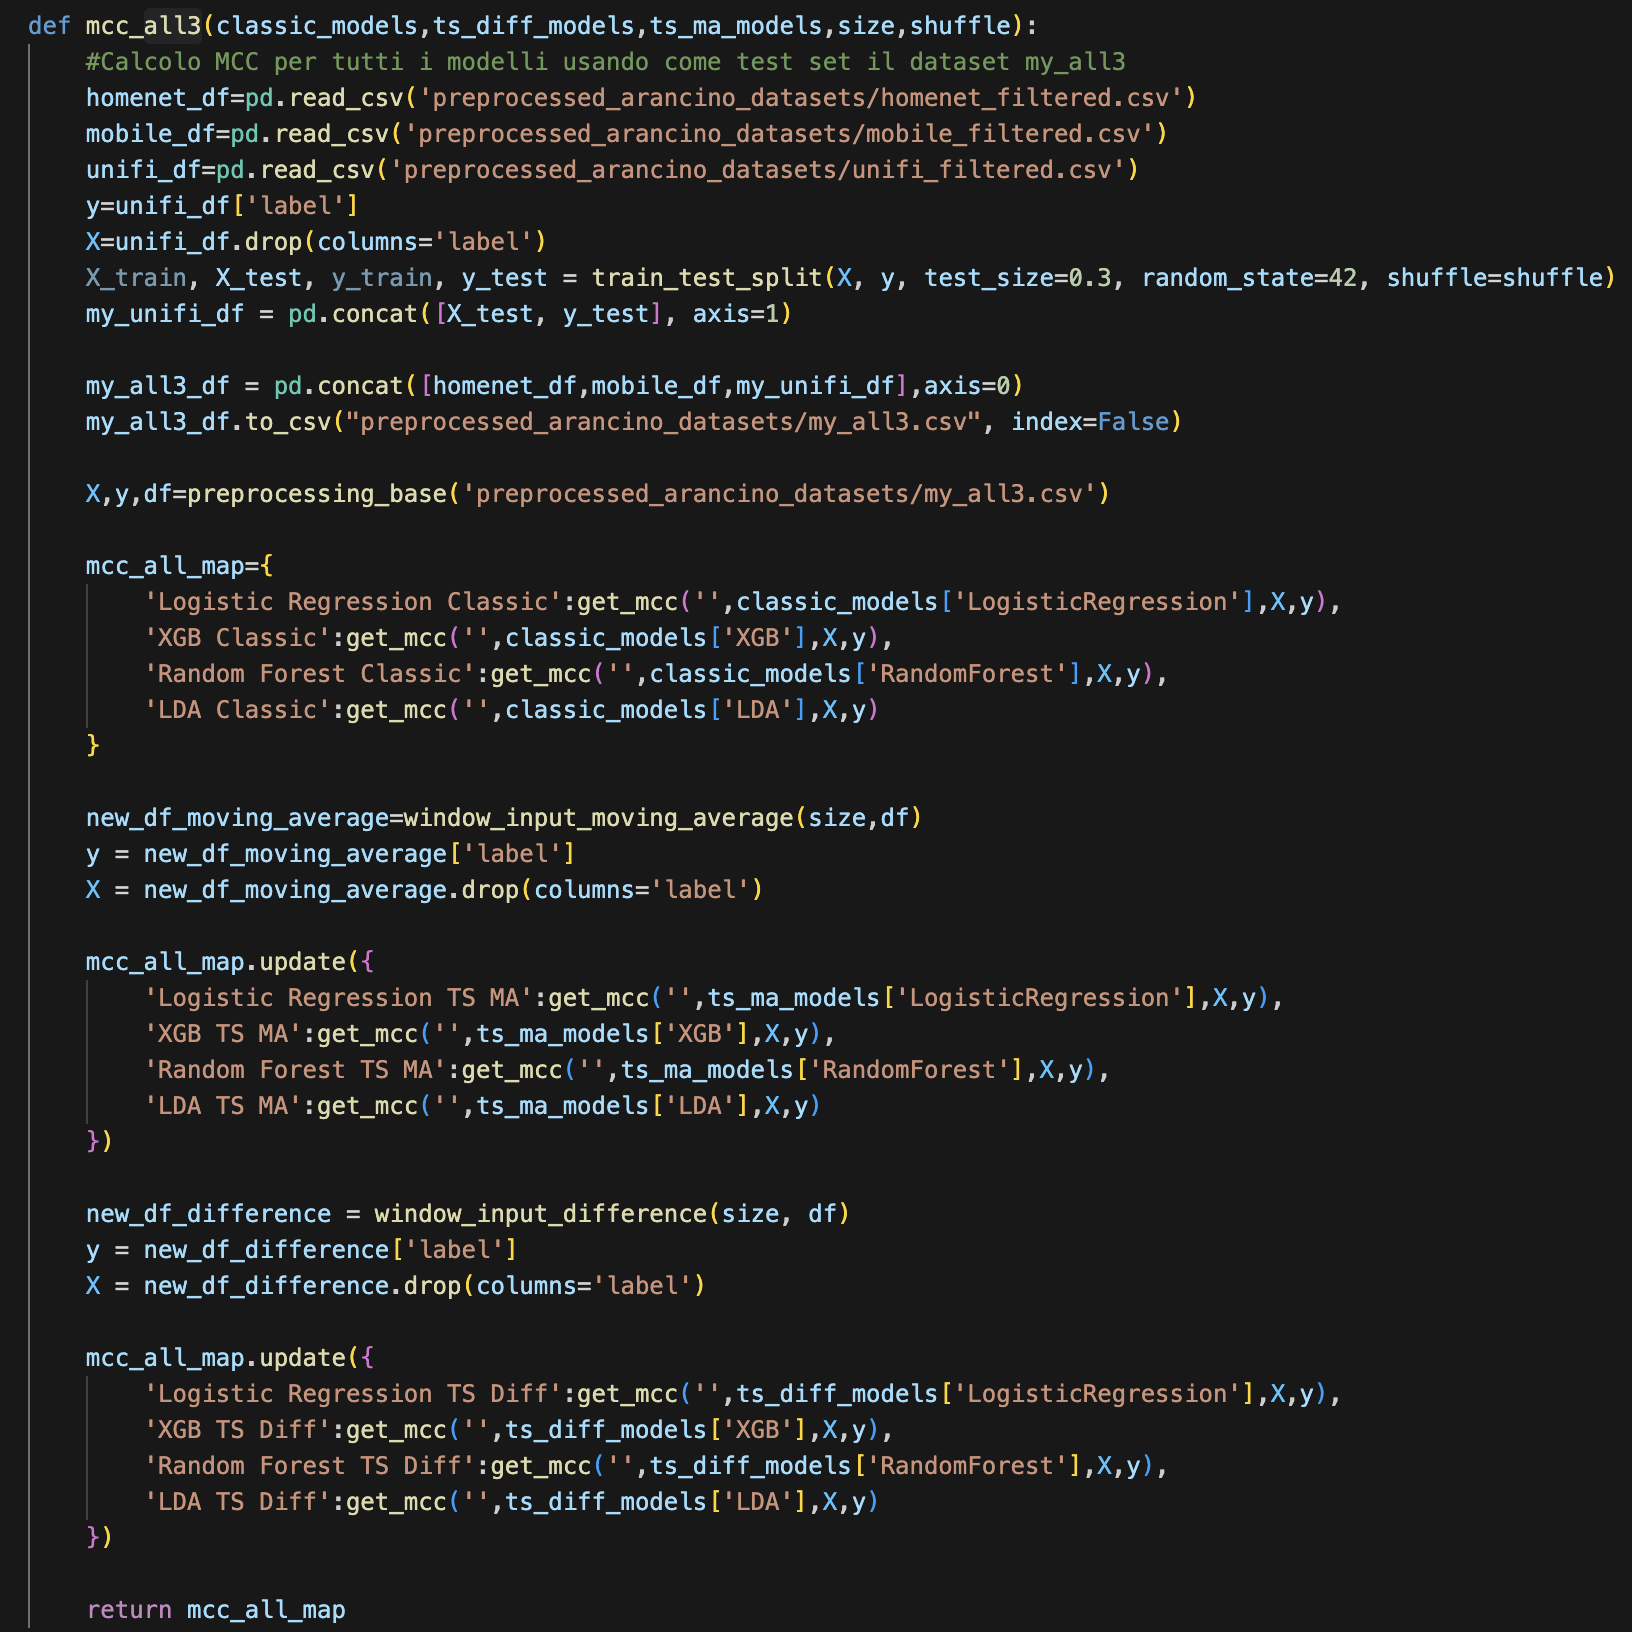
\includegraphics[width=1\linewidth]{23.png}
    \label{fig:enter-label}
\end{figure}

\begin{figure}[H]
    \centering
    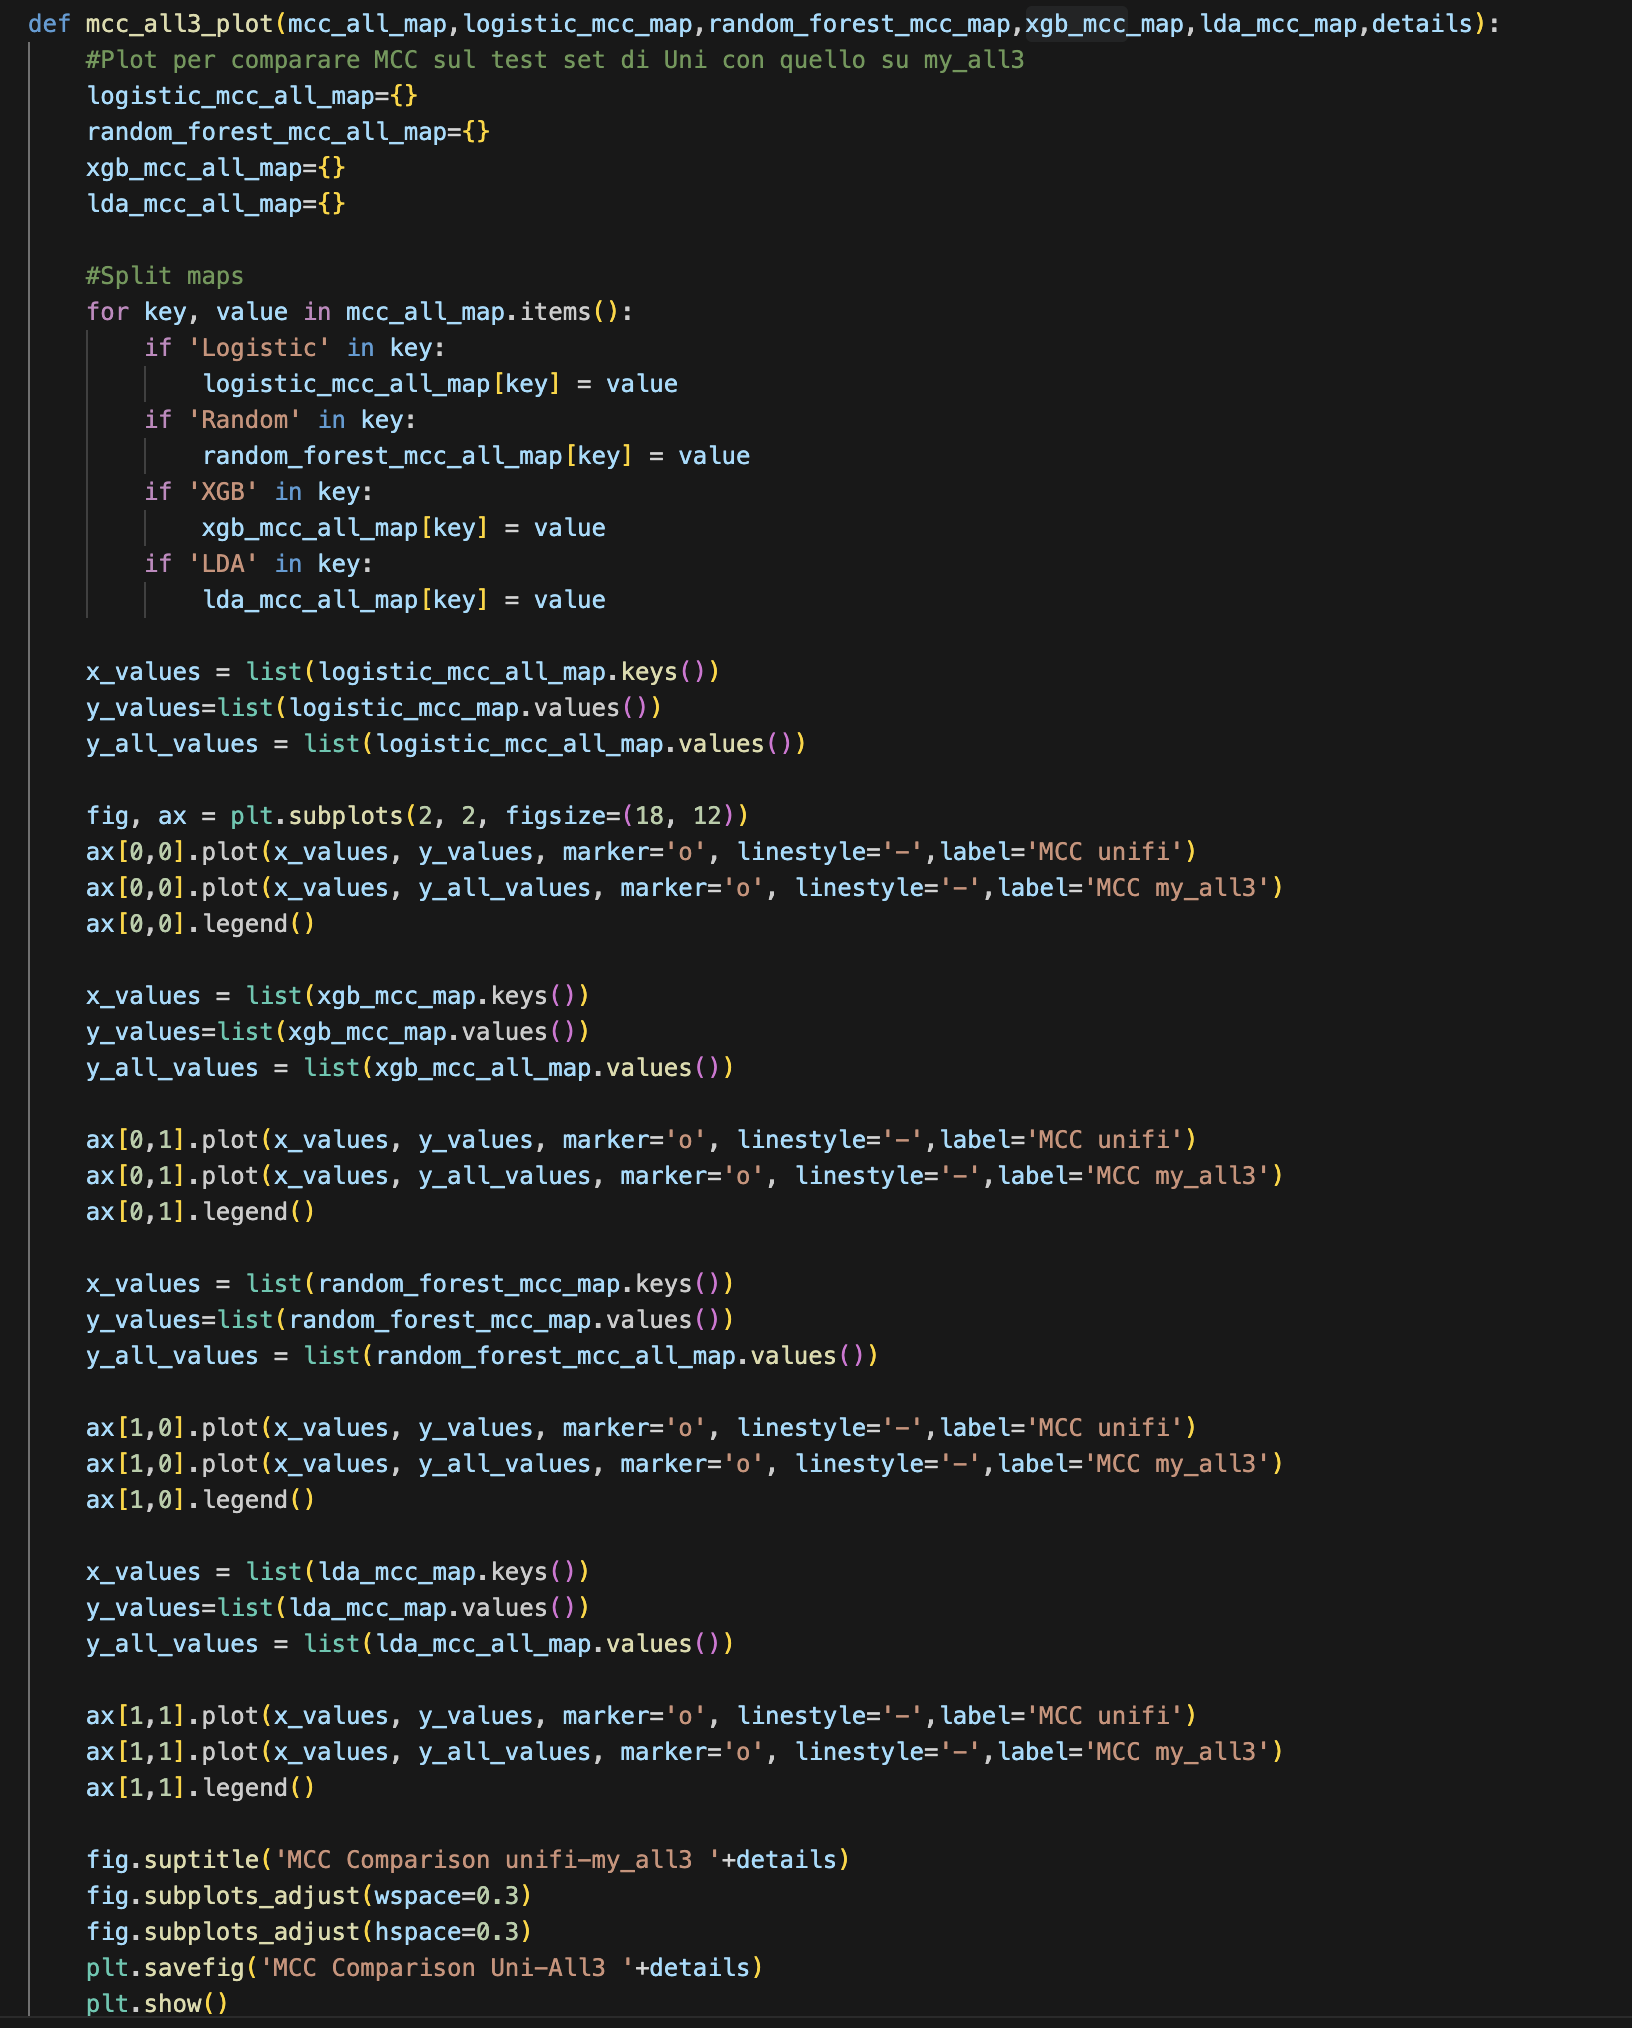
\includegraphics[width=1\linewidth]{24.png}
    \label{fig:enter-label}
\end{figure}

\begin{figure}[H]
    \centering
    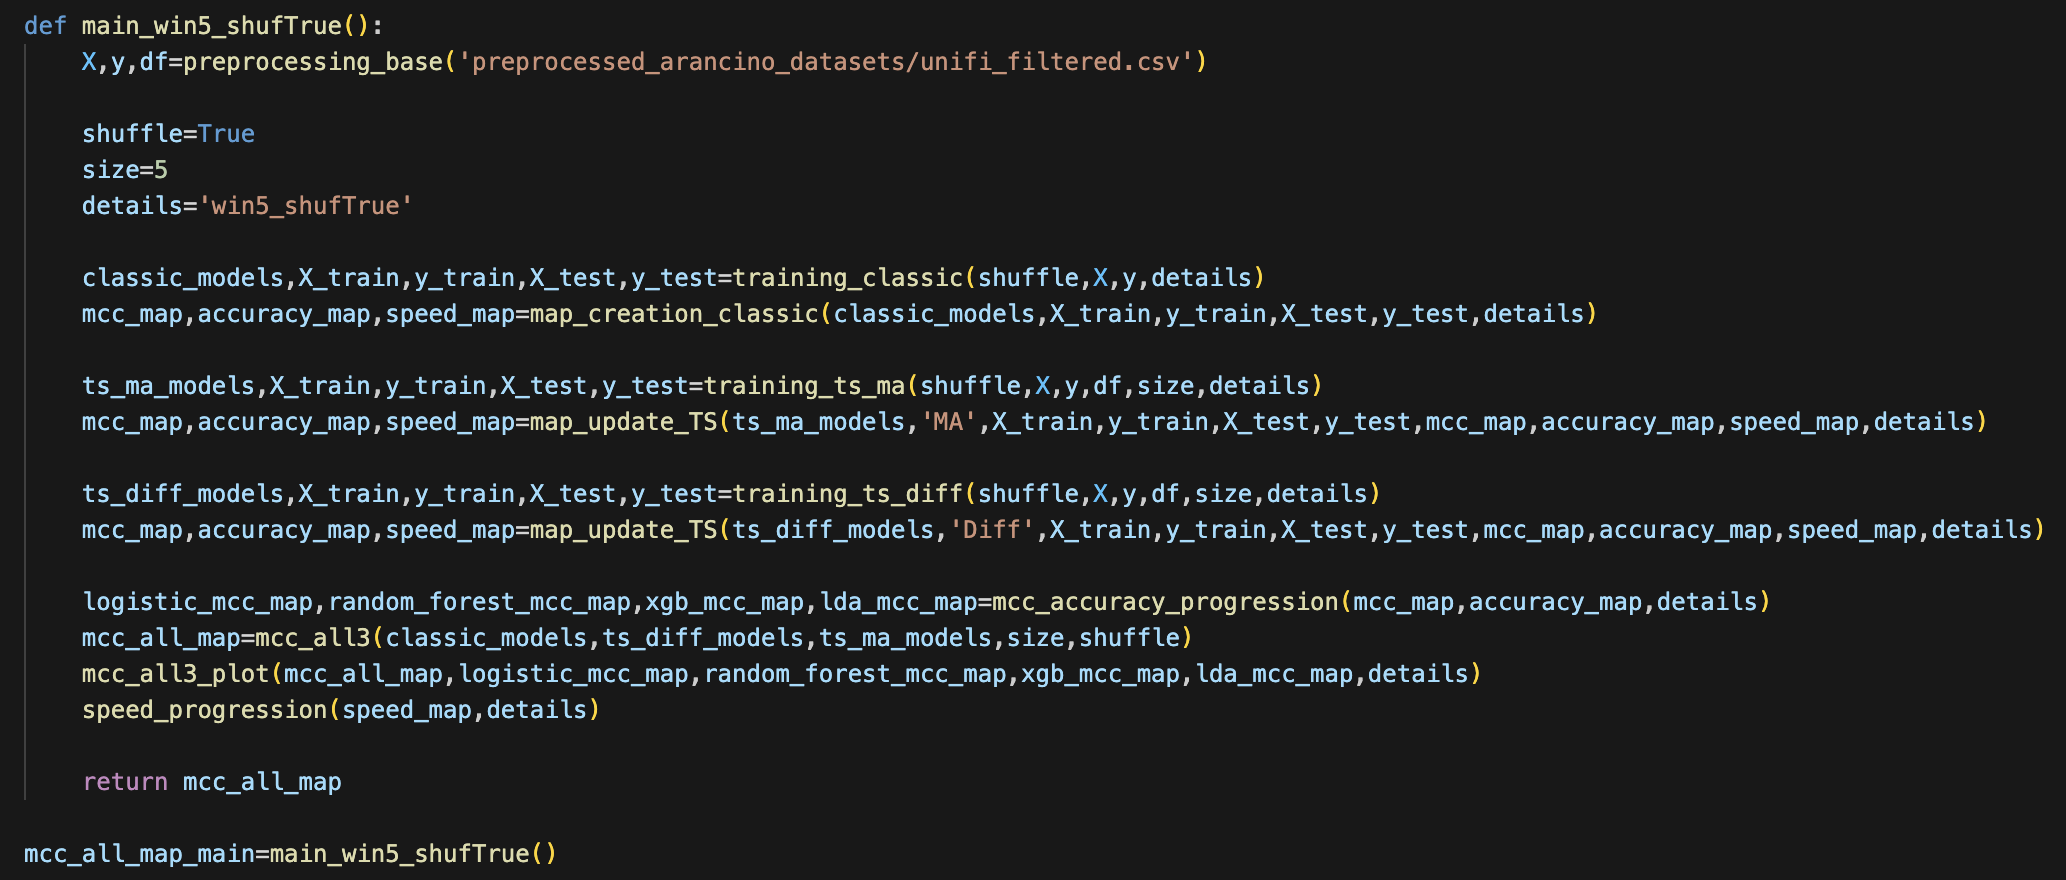
\includegraphics[width=1\linewidth]{25.png}
    \label{fig:enter-label}
\end{figure}

\begin{figure}[H]
    \centering
    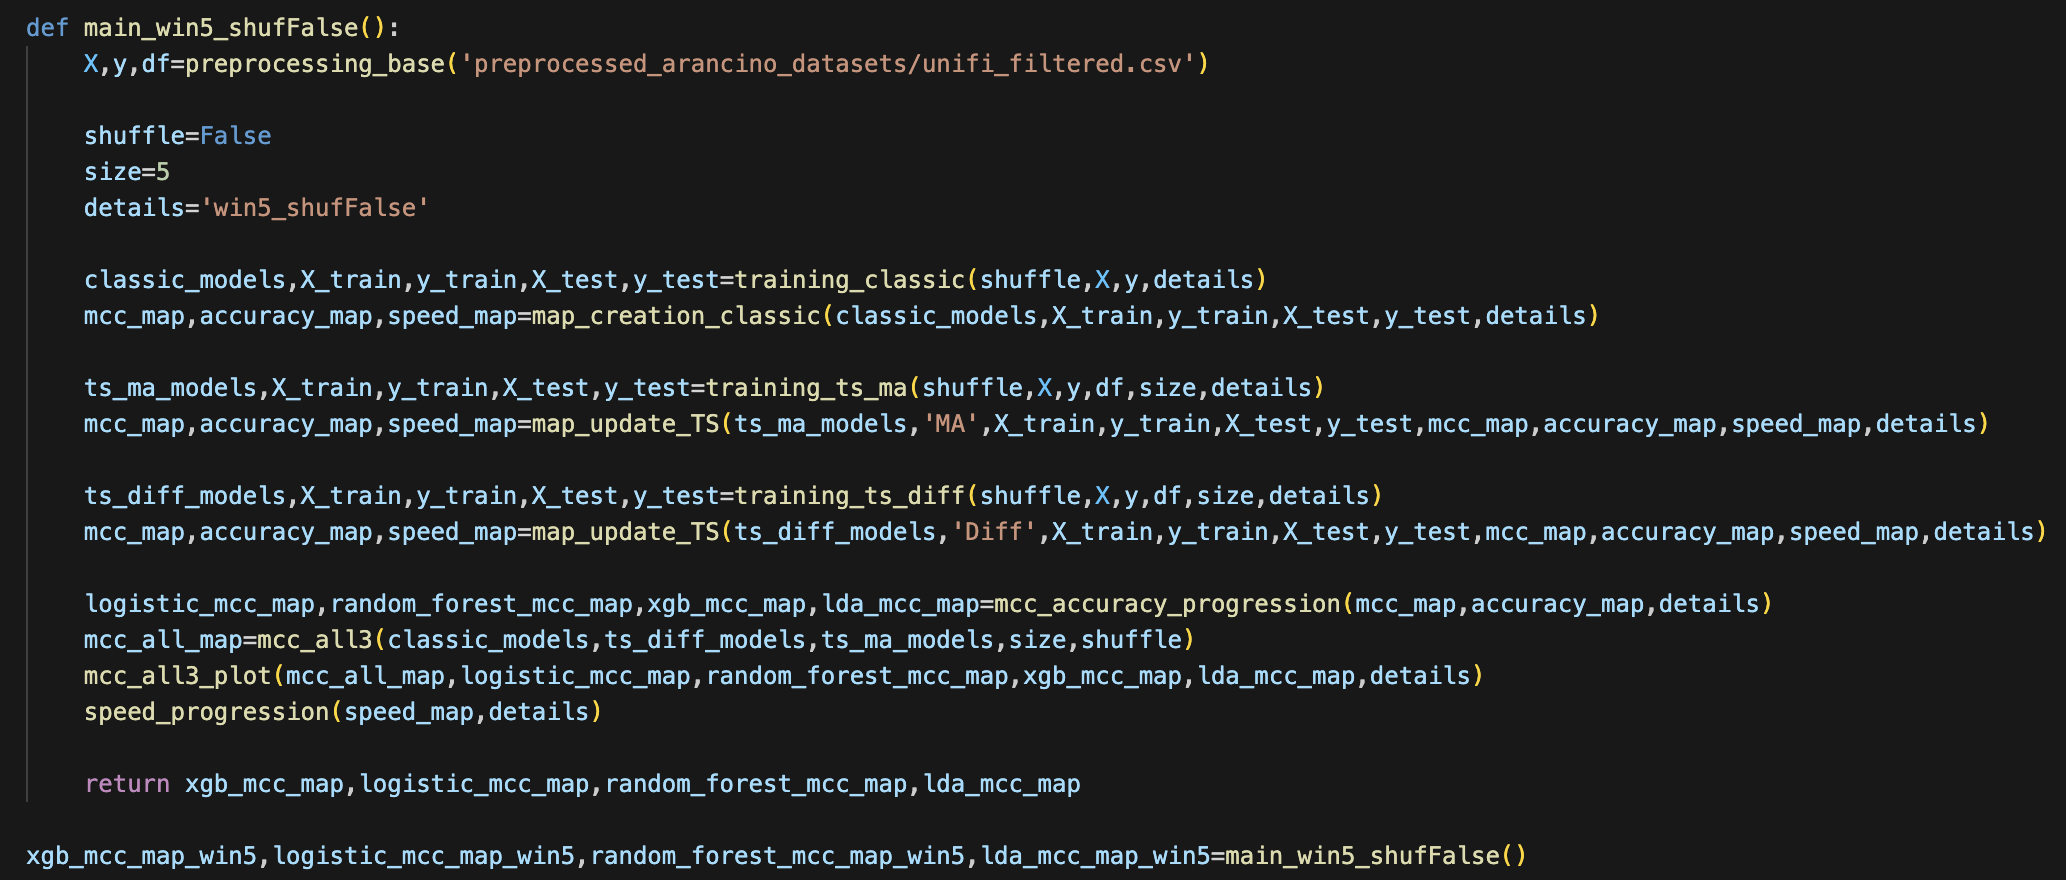
\includegraphics[width=1\linewidth]{26.png}
    \label{fig:enter-label}
\end{figure}

\begin{figure}[H]
    \centering
    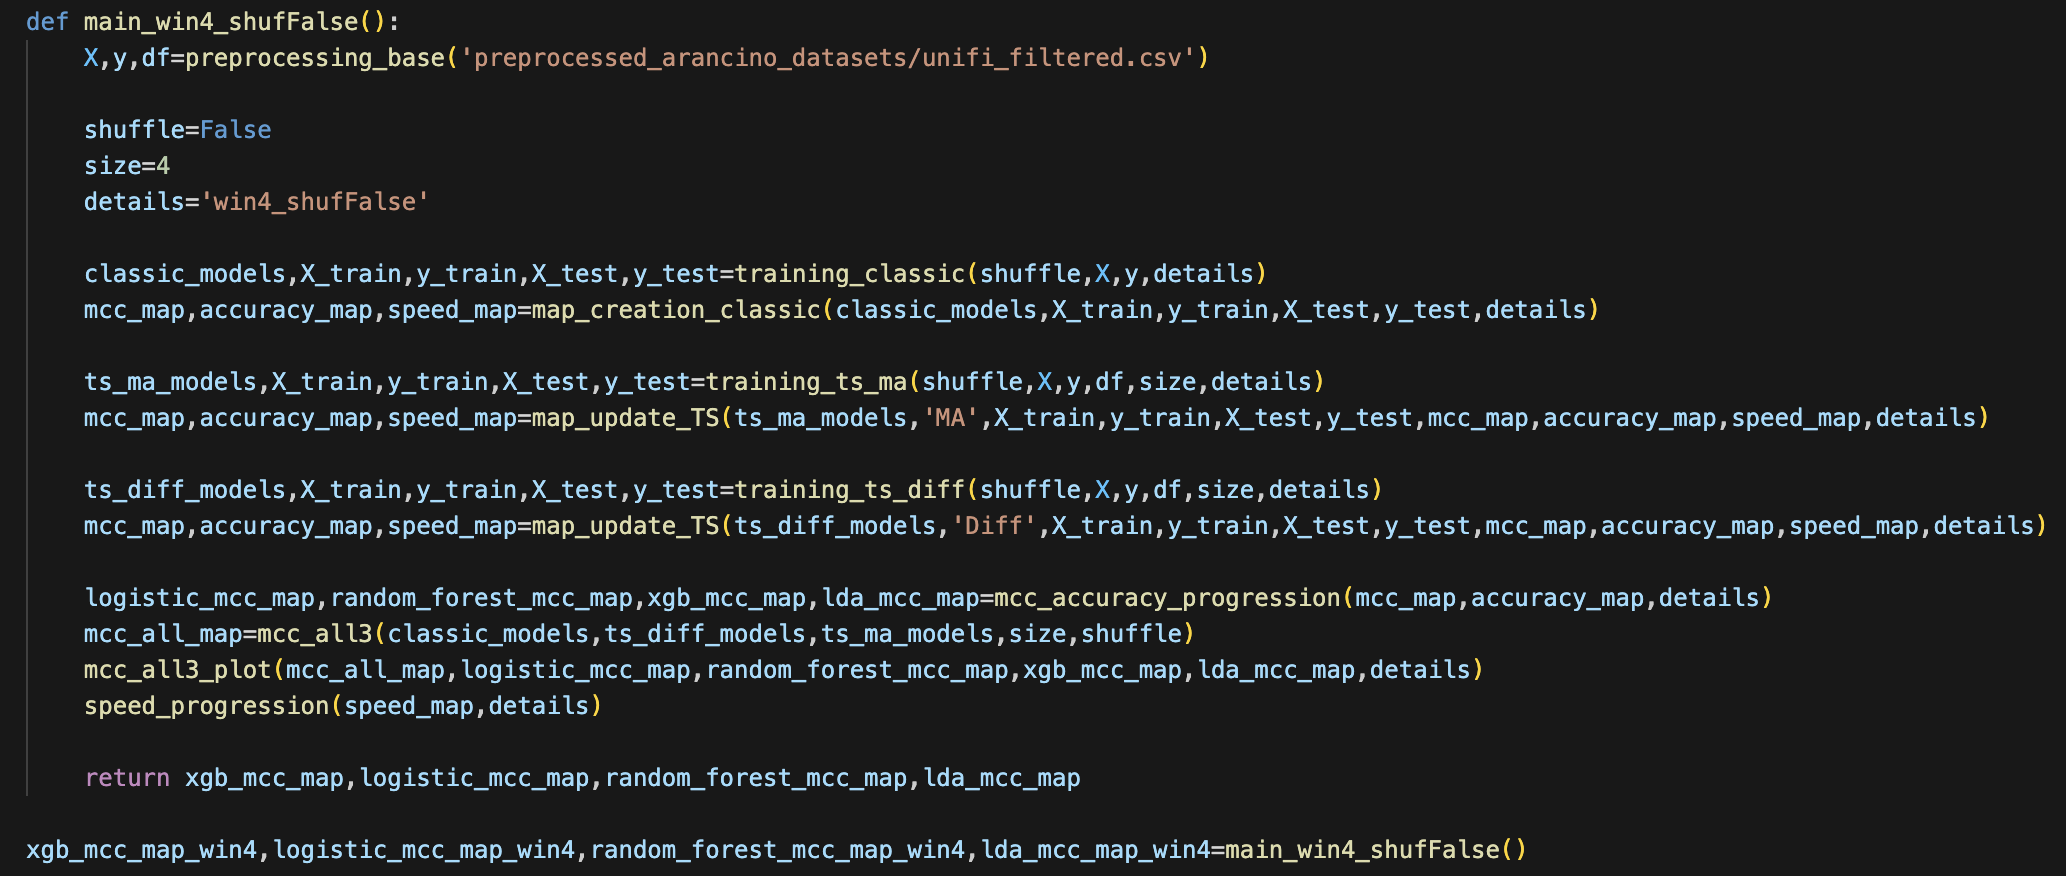
\includegraphics[width=1\linewidth]{27.png}
    \label{fig:enter-label}
\end{figure}

\begin{figure}[H]
    \centering
    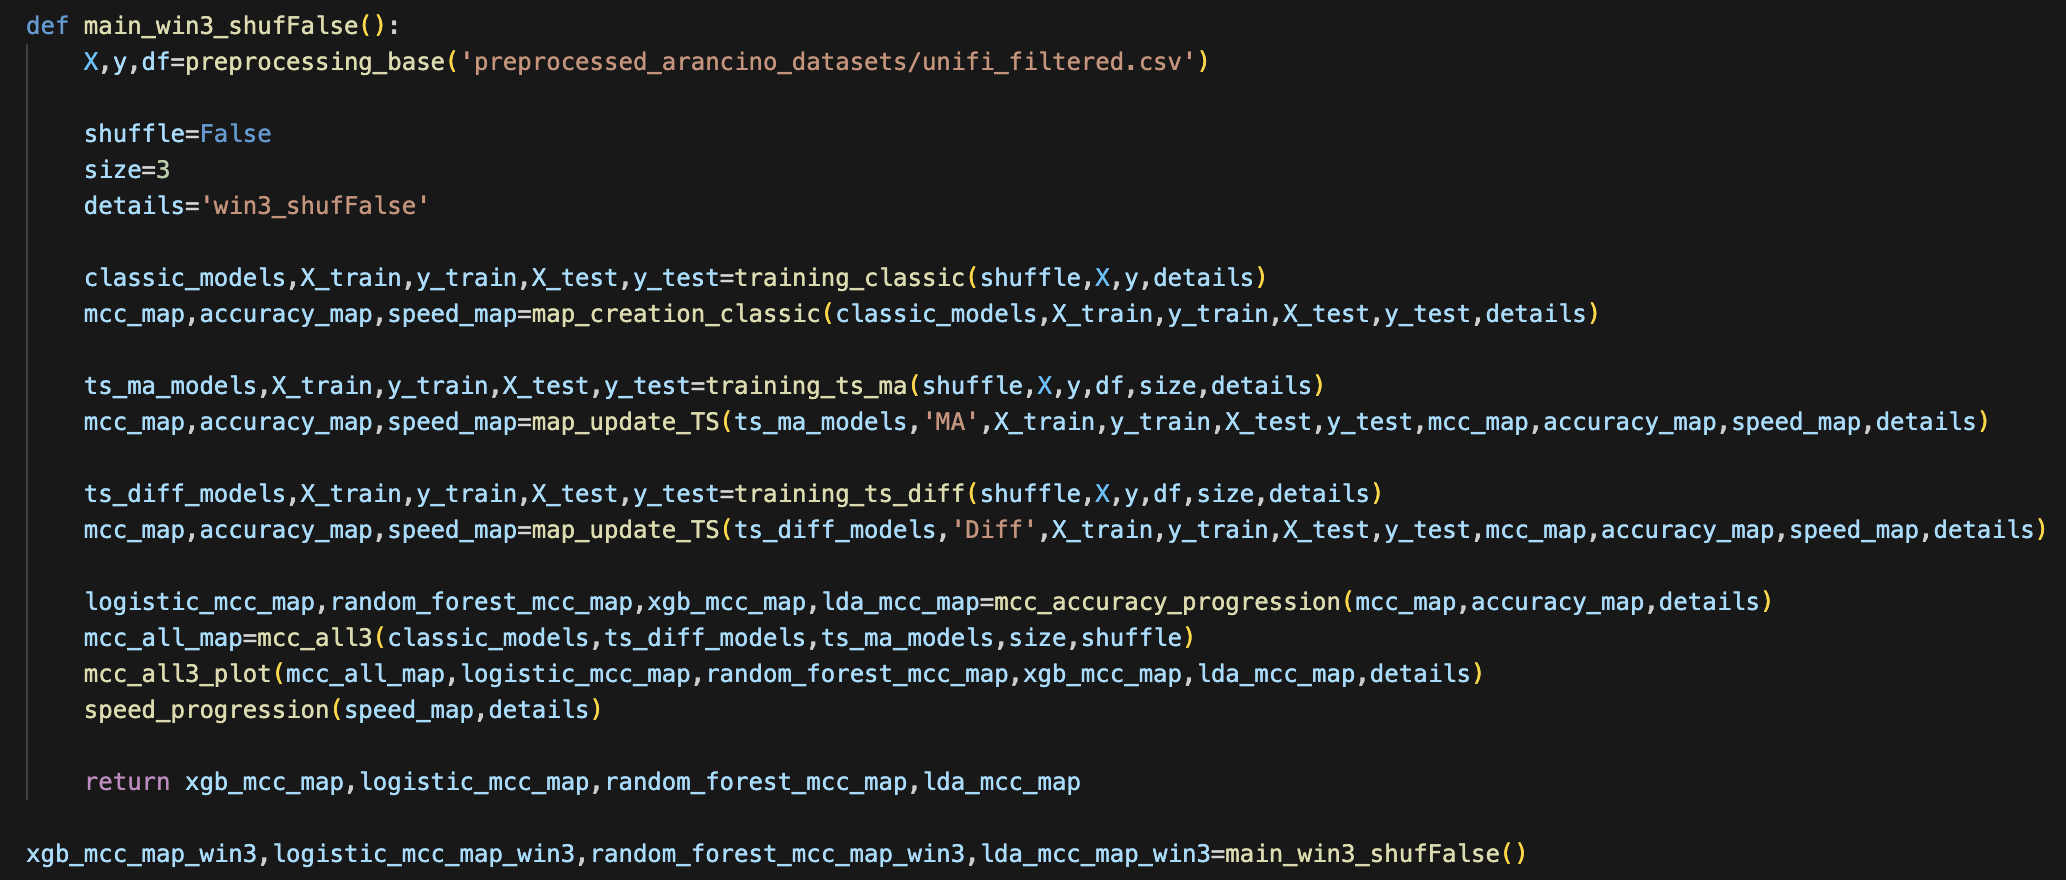
\includegraphics[width=1\linewidth]{28.png}
    \label{fig:enter-label}
\end{figure}

\begin{figure}[H]
    \centering
    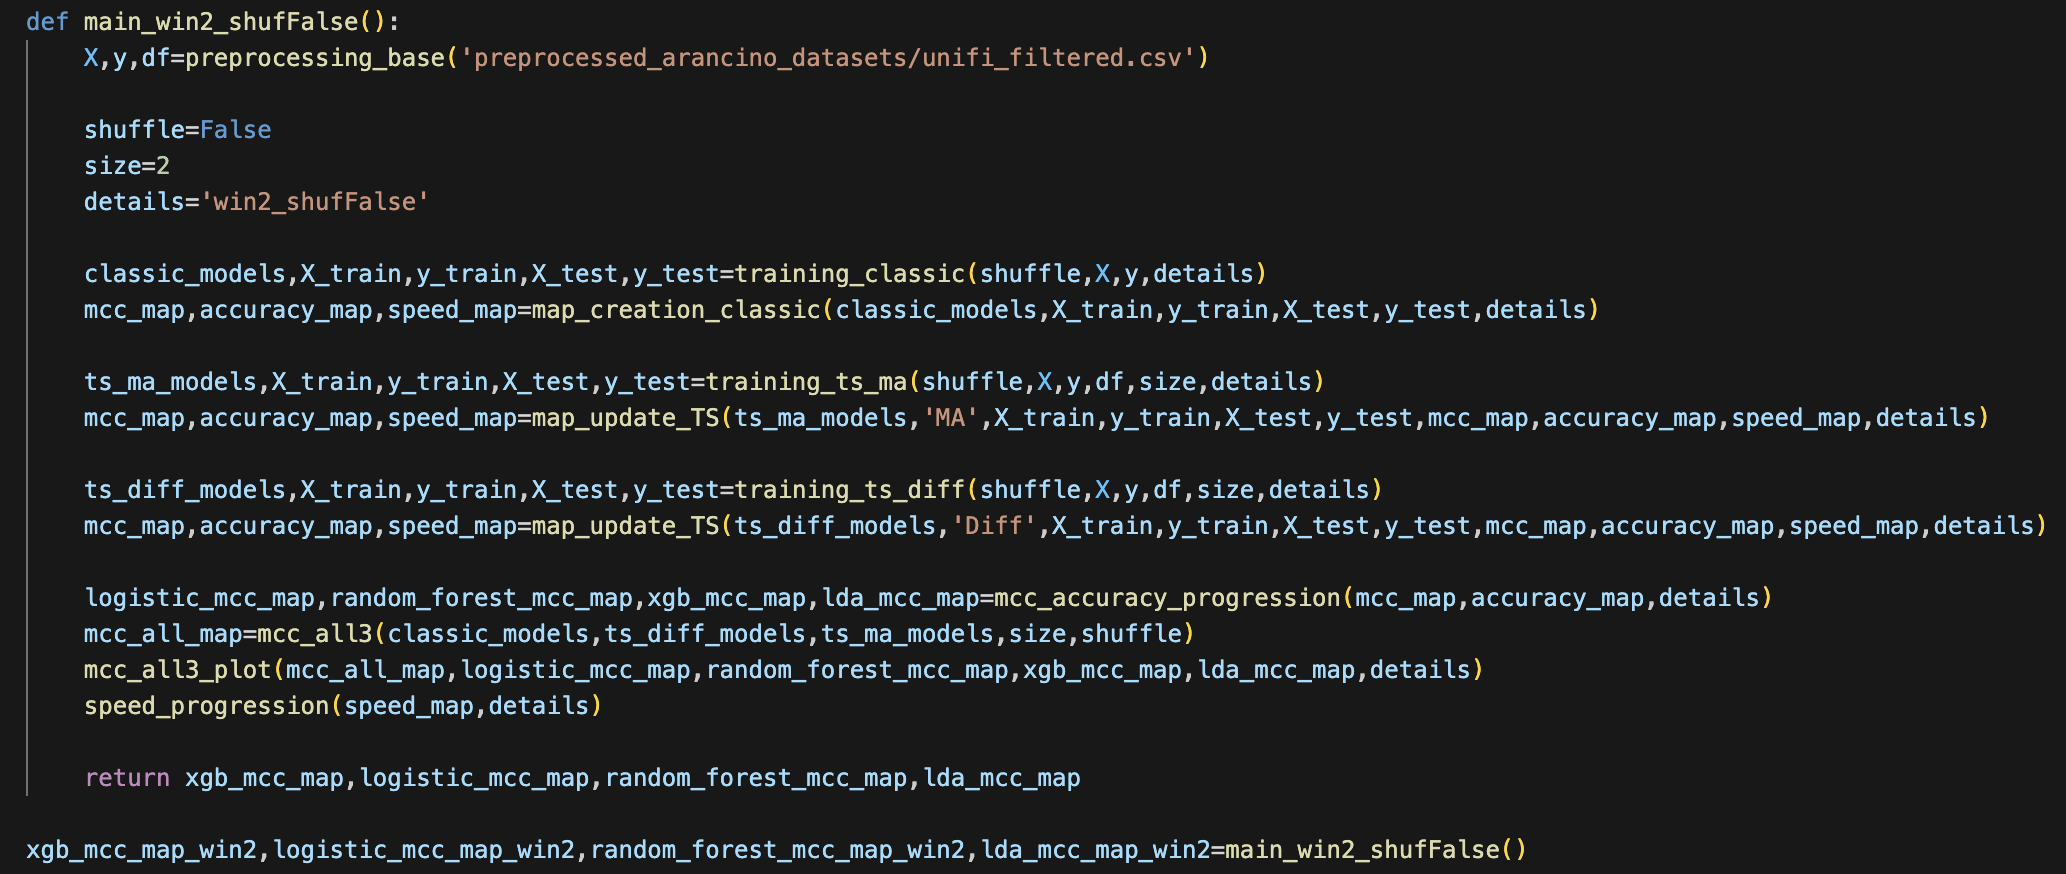
\includegraphics[width=1\linewidth]{29.png}
    \label{fig:enter-label}
\end{figure}

\begin{figure}[H]
    \centering
    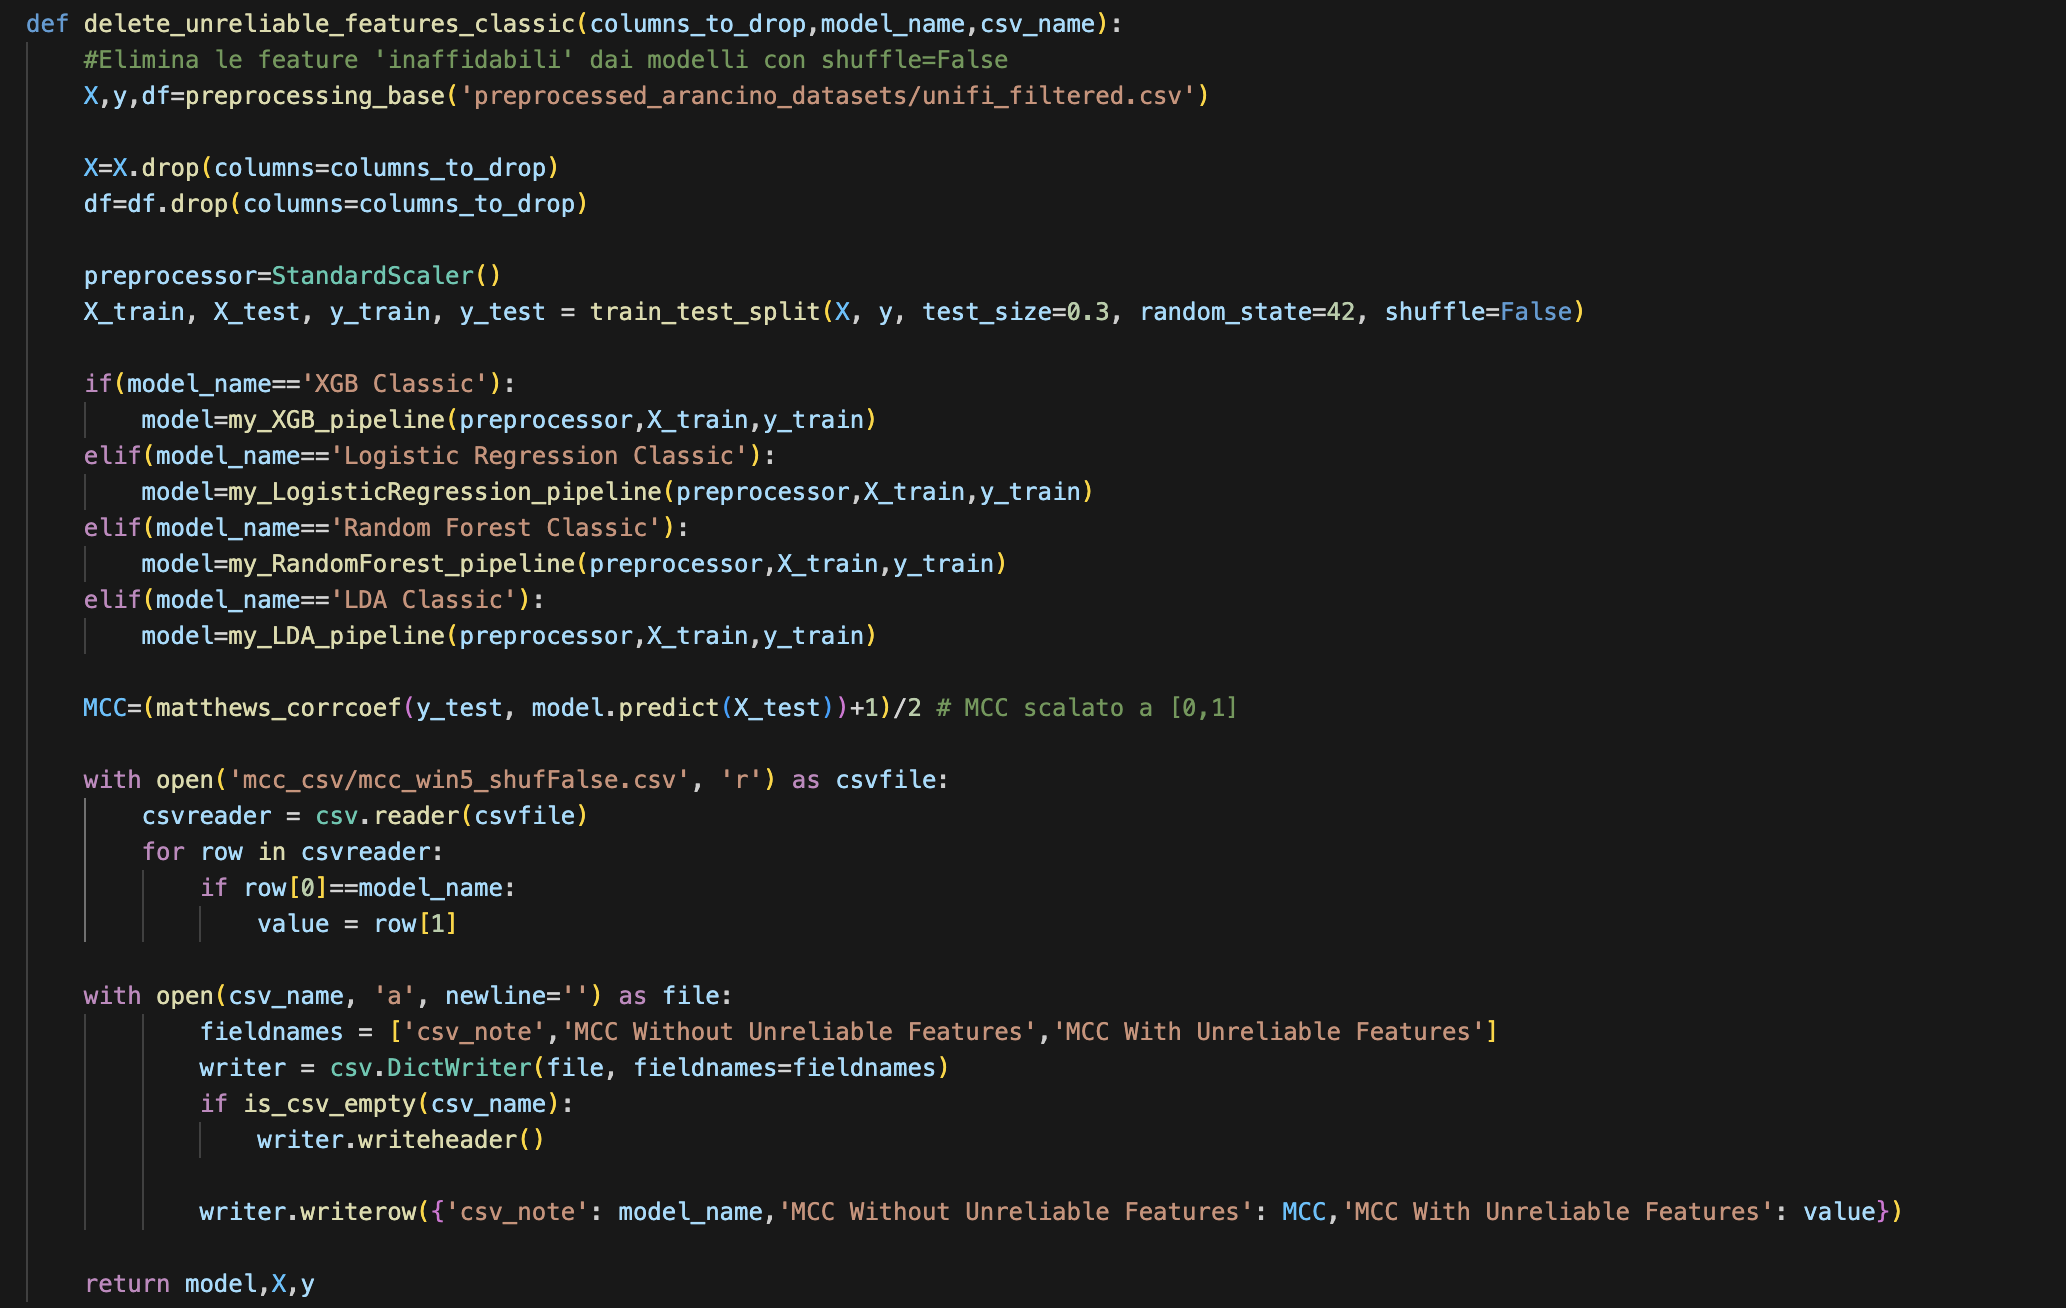
\includegraphics[width=1\linewidth]{30.png}
    \label{fig:enter-label}
\end{figure}

\begin{figure}[H]
    \centering
    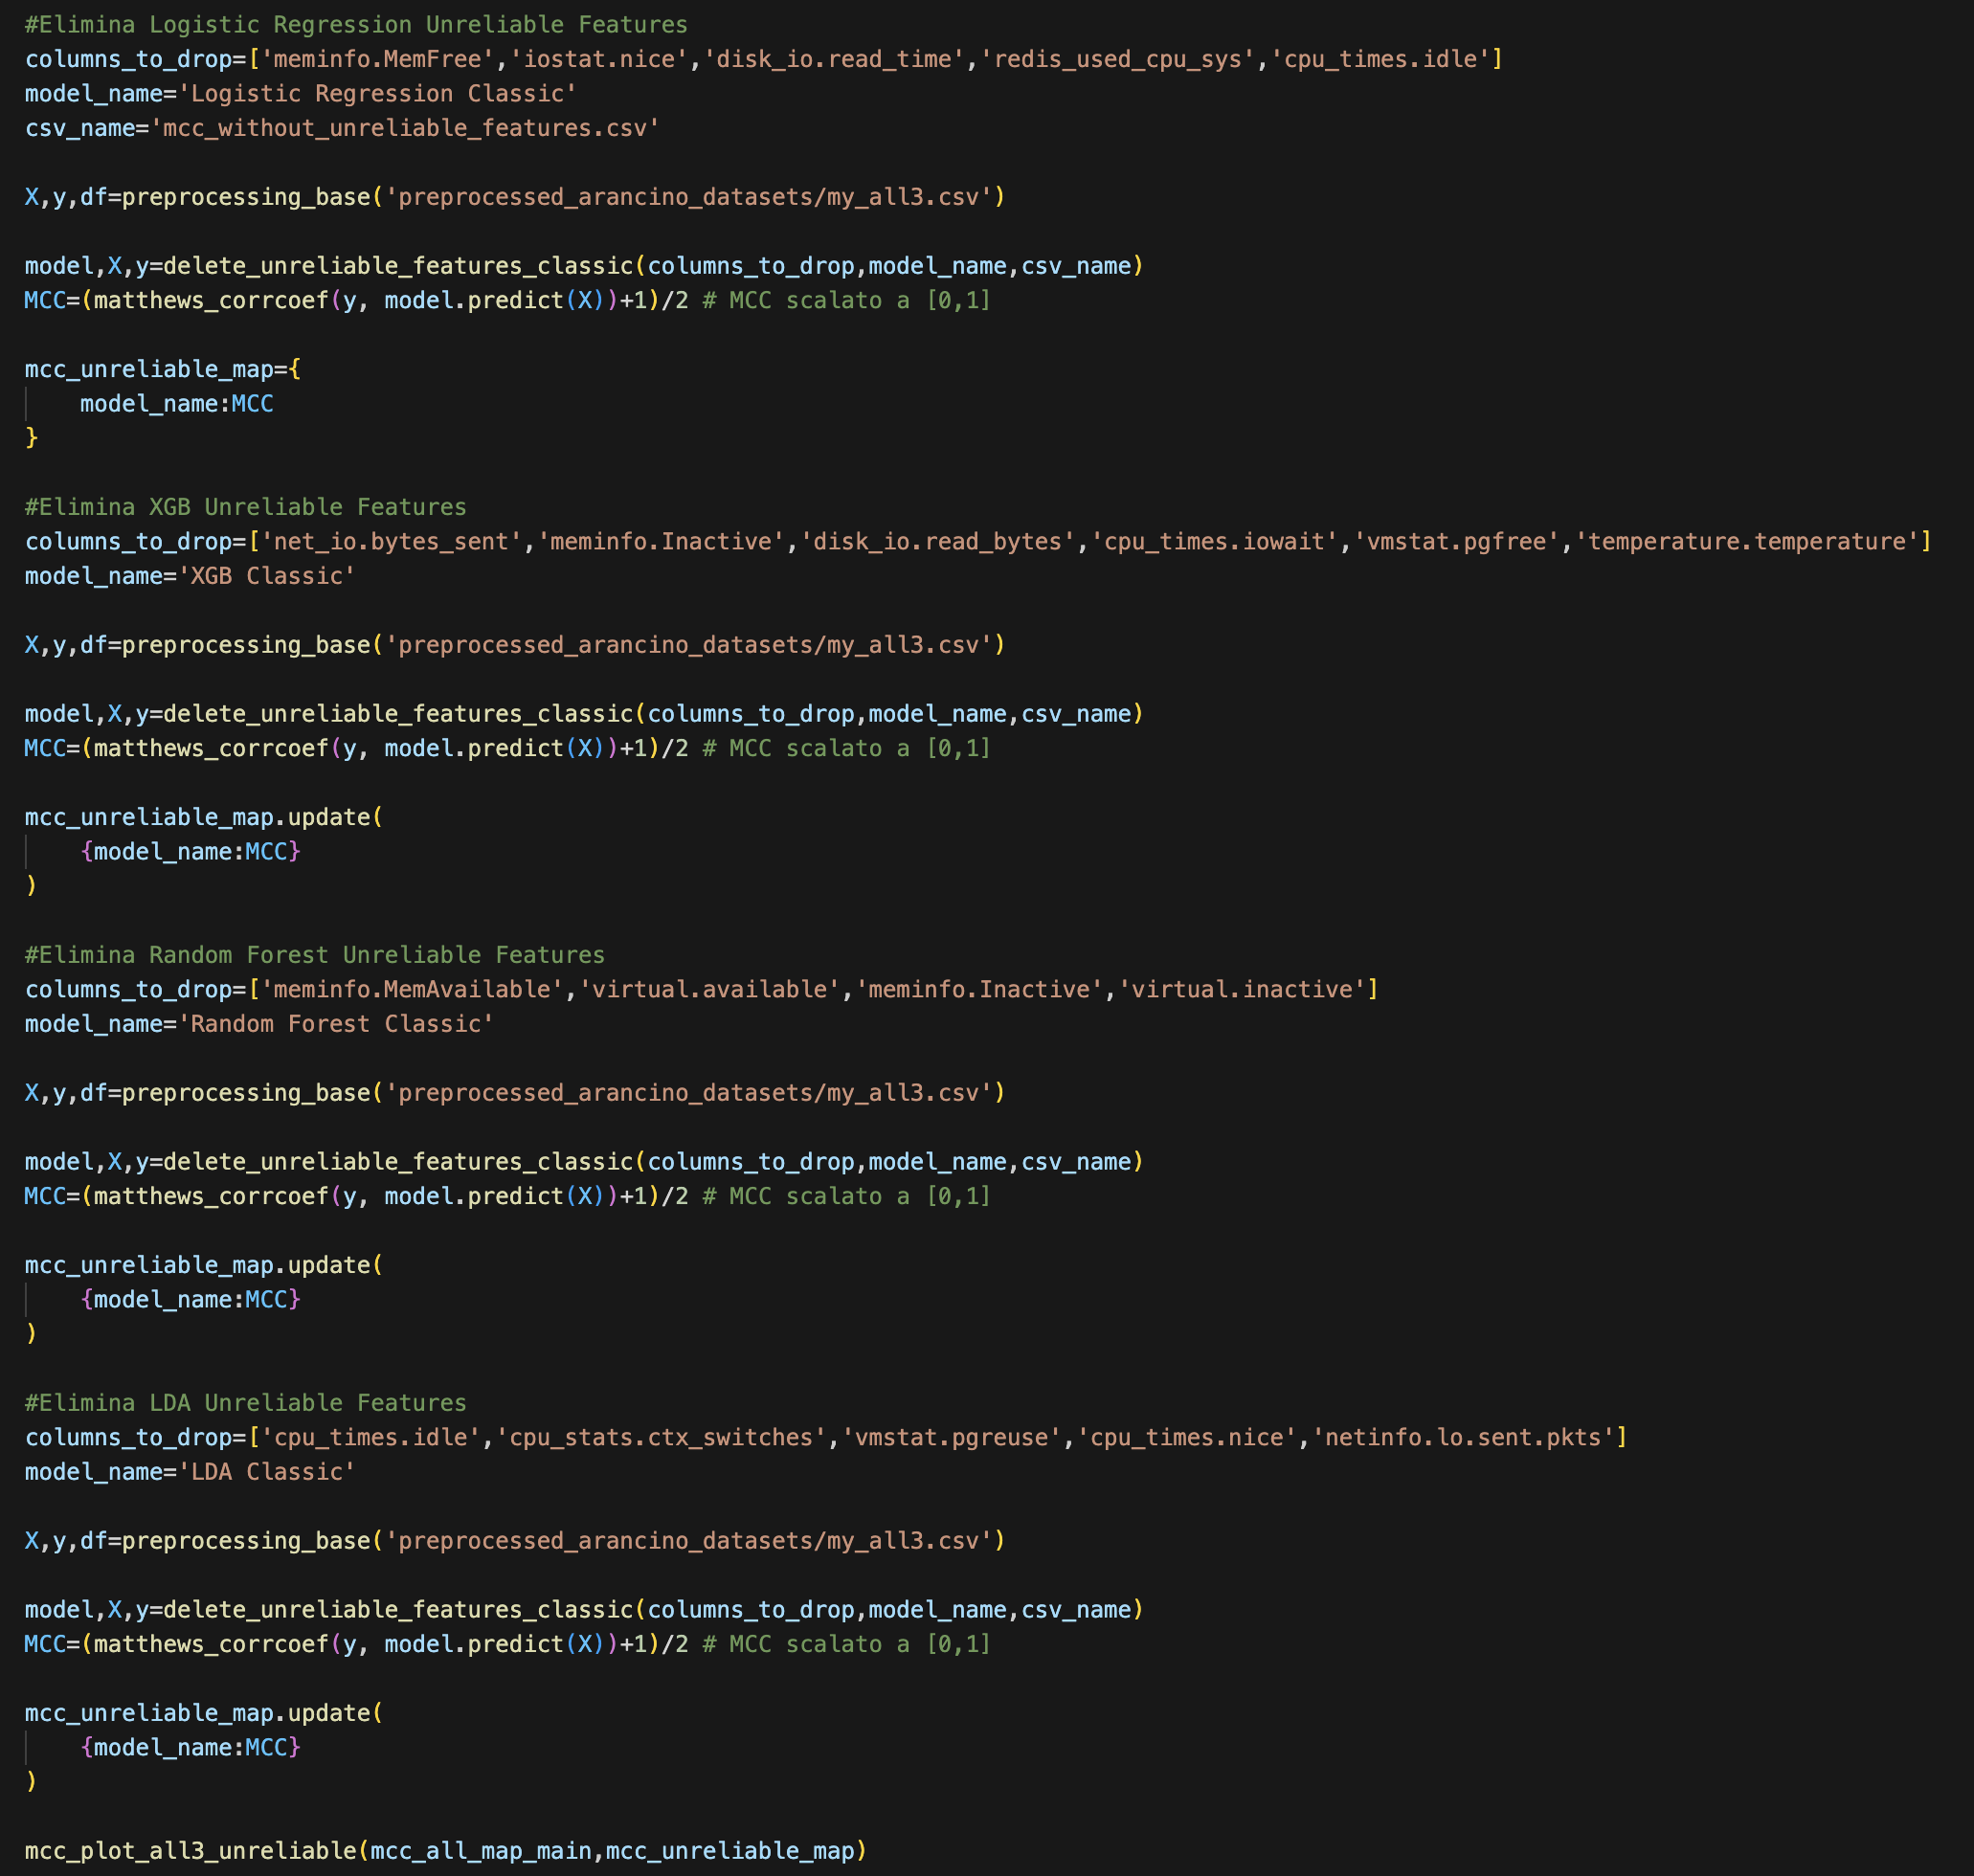
\includegraphics[width=1\linewidth]{31.png}
    \label{fig:enter-label}
\end{figure}

\begin{figure}[H]
    \centering
    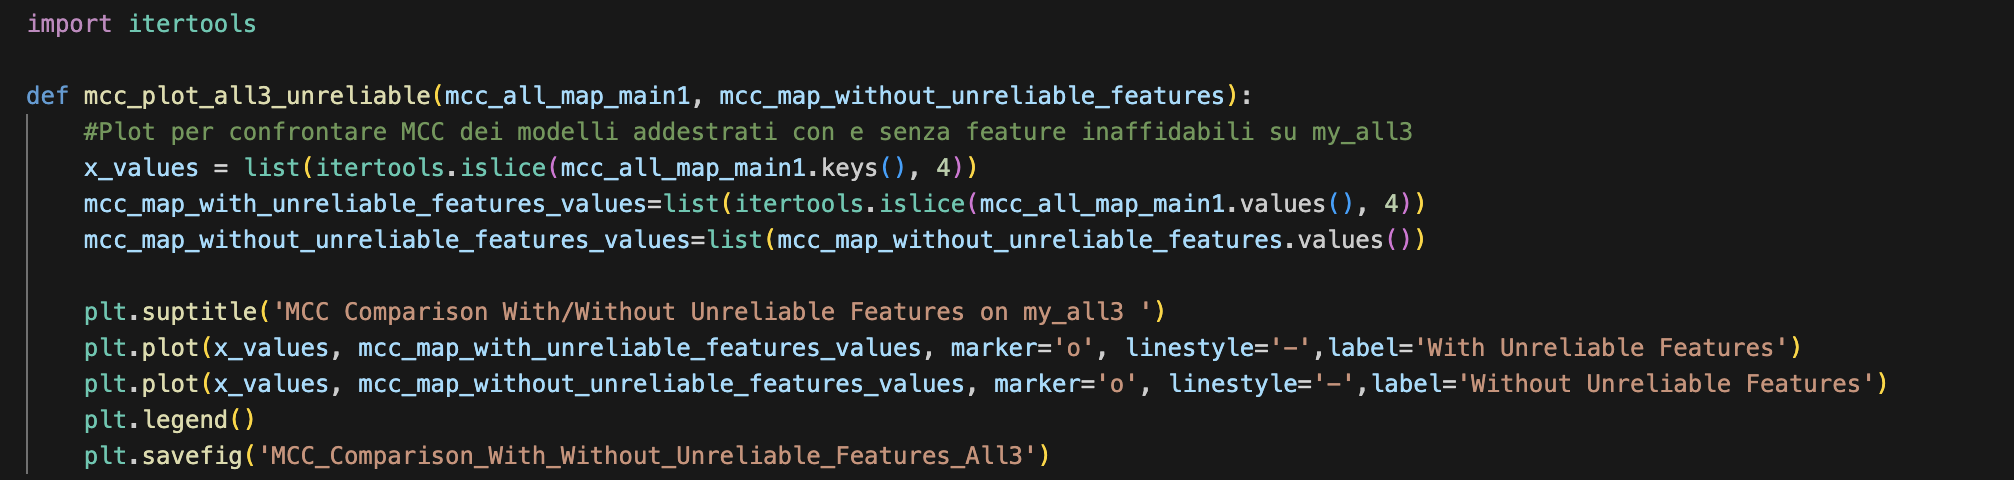
\includegraphics[width=1\linewidth]{32.png}
    \label{fig:enter-label}
\end{figure}

\begin{figure}[H]
    \centering
    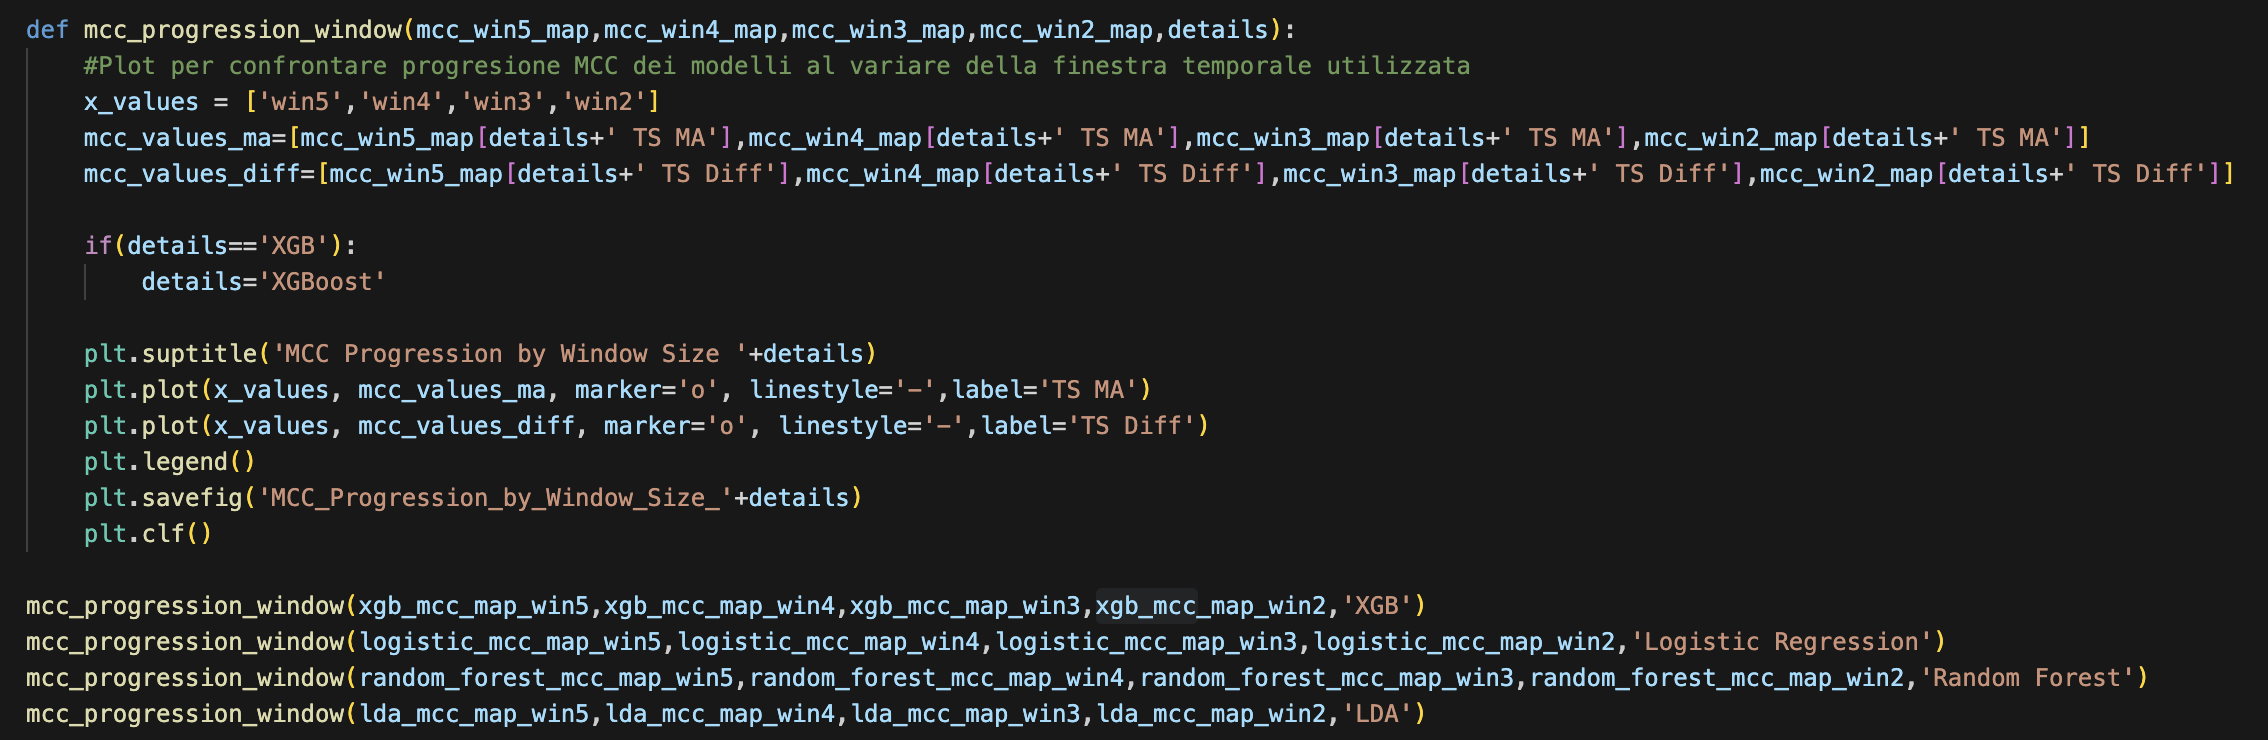
\includegraphics[width=1\linewidth]{33.png}
    \label{fig:enter-label}
\end{figure}
\end{appendices}
\bibliography{THESIS/bibliografia}
\end{document}
%--------------------------------------------------------------